% created on 28/07/2020
% @author : ebazan
\part{Global Color and Texture}\label{part:global_color_texture}%Image Global Color and Texture

\section*{Introduction}
In part \ref{part:image_contours}, we show that low-level features, such as image contours, provide useful perceptual information that can be used to solve complex problems. We presented a framework that uses the concepts of human perception and contour information for the unsupervised detection of landing targets. This framework is able to identify the marker under degraded operating conditions using only exogenous features from the contours, which are identified on gray-level images. The framework can be improved by adding other features that provide perceptual information of a scene.

In this part of the thesis, we review two more low-level image features: color and texture. Both features are widely involved in the perceptual process of humans and their study can be very extensive. The objective of this part is to explore the image color and texture features for their future integration into a general framework for object detection. Particularly, in this part of the thesis we are interested in the global distribution of color and texture information of an image. For this purpose, the chapter that opens this part seeks to remember recall the definition of color and texture in the field of computer vision. Moreover, it review different approaches to color representation as well as different strategies for characterizing texture features. Later, in chapter \ref{ch:similarity_measures}, we take interest at the comparison of distributions, particularly in the study of the Optimal Transport (OT) as a metric for the measurement of similarity between distributions and its application in the field of computer vision.

Throughout these chapters of the thesis, we address the study of those two properties using simple images containing the information of interest; in the case of color, images containing low color variation and; in the case of texture, grayscale images with homogeneous textures.

The main contributions of this part are:

\begin{enumerate}
	\item Review of the state of the art of global color representations and texture characterizations.
	\item Review of the state of the art of similarity measures, particulary the interpretation of the OT in computer vision: the Earth Mover's Distance (EMD).
	\item Qualitative and quantitative study between the most popular measures in the comparison of distributions and the EMD. 
	\item An unsupervised image retrieval system based on global color/texture information.
\end{enumerate}


\chapter{Global Representations of Color and Texture } \label{ch:color_texure_representations}

\section*{Résumé}
\noindent 
Ce chapitre présente une compilation des différentes manières de représenter les informations de couleur et de texture présentes dans une image. En ce qui concerne les informations de couleur, nous introduisons certains types d'espaces colorimétriques et leurs origines. De plus, nous présentons quelques techniques pour synthétiser ces informations. Dans le cas de la texture, nous présentons les différentes méthodologies pour son étude, en mettant en évidence les avantages et les inconvénients de chaque méthode.
\section*{Abstract}
\noindent 
This chapter presents a compilation of the different ways of representing the color and texture information present in an image. When it comes to color information, we present some of the most popular color spaces used as well as their origins and relationship to human perception. In addition, we present some techniques to synthesize this information. In the case of texture, we present the different methodologies for its study, highlighting the advantages and disadvantages of each method. 

\section{Introduction}

If we look around us, we can see that many of the materials and objects of yhe environment only exist with certain colors. For example, the clouds are mostly  white, the grass is green, the ocean is blue, etc. Performing the same experience, but this time with textures, we realize that we are surrounded by them everywhere. We find textures, for example, at textiles, buildings, tilings and on skins or objects surfaces. The color and texture of an image is very valuable information and therefore, the perception of such information is a powerful tool for classifying and recognizing certain objects and materials.

For decades several vision algorithms have sought to exploit this information. Color and texture are of relevant importance for its use as a feature to characterize objects. Due to these facts, the definition and the various representations of the color, as well as the texture information, is addressed in this chapter. As far as color information is concerned, we give a brief introduction to what color is and how it can be represented. In the case of texture, we present a brief introduction to textures including its types and an overview to the various methodologies for its study, highlighting the advantages and disadvantages of each method. 


\section{Color}
The study of color is one of the most perplexing and interesting subjects in vision. Although the understanding of the basic concept of the color spectrum is easy to explain, the theory of color is an infinitely more complex subject that has scientific and artistic origins. For example, Newton was interested in the physical properties of color and discovered, with his famous experiment of the light beam projected on a prism, that white light is a combination of all colors across the color spectrum \citep{Newton:Book:1704}.  On the other hand, authors like Goethe dedicated their work about color to a more human-centered analysis of the perception of this information through a series of experiments that measure the response of the eyes to certain colors \citep{Goethe:Book:2015}.

Today we know that the electromagnetic spectrum visible to humans is between 380 and 750 nm (see figure \ref{fig:visual_spectrum}). The electromagnetic radiation between this range of wavelenghts is what we call visible light or simply light. Therefore, we can define color as the main property of visible light by which a human observer can distinguish different kinds of light \citep{Kerr:Online:2003}.

From a biological point of view, we are able to perceive different colors thanks to the human visual system (HVS) composed, roughly, by the eye's elements such as the retina and its photoreceptors (cones and rods); the nervous system and; the part of the brain that interprets information \citep{Fairchild:Book:2005}. The cones are the main photoreceptors for color vison because they work when more light is available, whereas rods are active in low illumination conditions. The three types of cones we have are properly referred to as L, M and S since they are sensitive to different wavelengths of light; long, medium and short wavelengths, respectively.

The figure \ref{fig:color_images} shows different examples of color images. Specifically, the image on the left is said to be synthetic because it is a man-made image where the colors encode the perceptual information in the image. The remaining three images are natural images that show the importance of color information since many elements of nature have a specific color representation distribution.

\begin{figure}[!ht]
    \centering
    \begin{subfigure}[b]{0.24\textwidth}
        
\includegraphics[width=\textwidth]{tempo}
        \caption{}
        \label{fig:tempo}
    \end{subfigure}
    %~ %add desired spacing between images, e. g. ~, \quad, \qquad, \hfill etc. 
      %(or a blank line to force the subfigure onto a new line)
    \begin{subfigure}[b]{0.24\textwidth}
        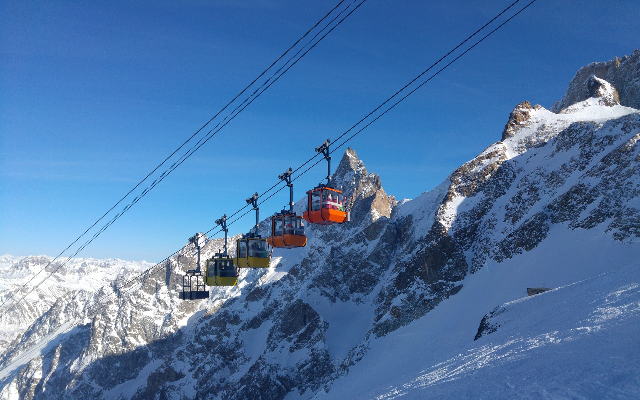
\includegraphics[width=\textwidth]{mountain}
        \caption{}
        \label{fig:parrots}
    \end{subfigure} 
    %~ %add desired spacing between images, e. g. ~, \quad, \qquad, \hfill etc. 
      %(or a blank line to force the subfigure onto a new line)    
    \begin{subfigure}[b]{0.24\textwidth}
        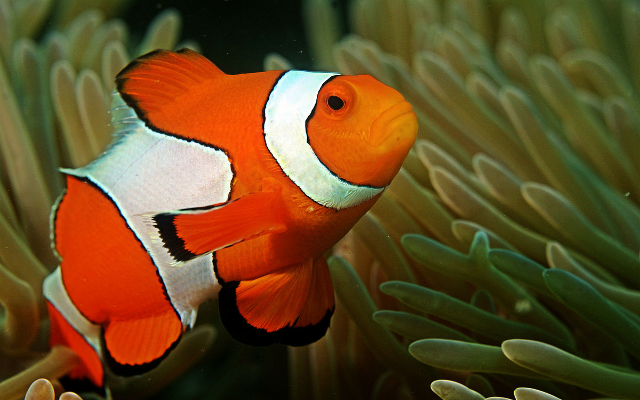
\includegraphics[width=\textwidth]{clownfish}
        \caption{}
        \label{fig:clownfish}
    \end{subfigure}
    %~ %add desired spacing between images, e. g. ~, \quad, \qquad, \hfill etc. 
      %(or a blank line to force the subfigure onto a new line)
    \begin{subfigure}[b]{0.24\textwidth}
        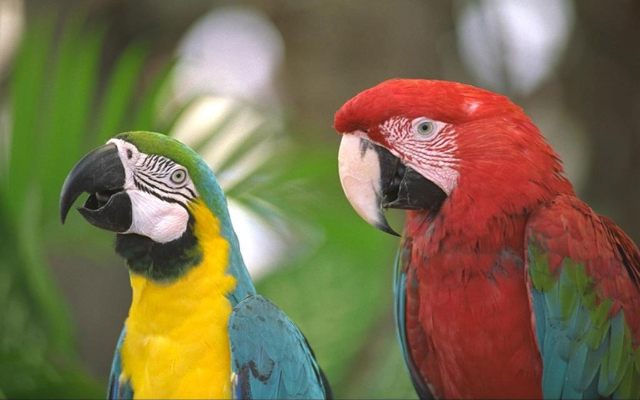
\includegraphics[width=\textwidth]{araras}
        \caption{}
        \label{fig:mountains}
    \end{subfigure}
                  
    \caption{Some examples of color images: One synthetic image {\small \textsf{\textbf{(a)}}} and three natural images [{\small \textsf{\textbf{(b) (c) (d)}}}].}\label{fig:color_images}    
\end{figure}


\subsubsection{Color theory}
Historically, there have been several attempts to explain the HVS and interpret its function in color vision. Two of the most popular theories of the mechanism of color vision are the trichromatic theory and the opponent-colors theory \citep{Fairchild:Book:2005}. The first of these, proposed by Maxwell, Young, and Helmholtz \citep{Young:PTRSL:1802, VonHelmholtz:Book:1867}, is based on the fact that we have three types of receptors (L-M-S cones). They assume that the receptors are roughly sensitive to the wavelengths of the red, green, and blue colors. Consequently, this theory simply suggests that each type of receptor generates an image which is weighted by the brain in order to sort out the color appearances.

The second theory is based on Hering's subjective observations \citep{Hering:Book:1878}. In his experiments, he noted that certain hues were never perceived to occur together. For example, color perception was never described as reddish-green or yellowish-blue. This suggested to him that the red – green and yellow – blue color pairs had something fundamental that caused them to behave like opponent colors. 
This theory gained strength in the mid-20th century where, supported by quantitative data, the stage theory emerged. This modern theory suggests that color perception is done in two stages. The first stage coincides with the trichromatic theory, so the LMS cones generate three color-separation images, however, in the second stage, the neurons of the retina encoded the colors into opposing signals \citep{Fairchild:Book:2005}. 

\subsection{Color representations}
Human color perception depends on the amount and wavelength of light captured by the eyes. Therefore, perceived colors can vary due to several factors such as the type of surfaces (or objects) where the light is reflected; the environment and even; the eyes of the observer. However, it is definite that the perception of color is an entirely arbitrary creation of our nervous system, and it is not contained in the wavelengths or in light-reflecting objects and materials \citep{Goldstein:Book:2009}. In other words, the interpretation of this information is completely subjective. A clear example of this is the naming of colors. When an incident spectrum contains all frequencies in the range of visible wavelengths, humans perceive objects that reflect all frequencies as clear, luminous or \textit{white}. In the opposite case, when the material absorbs and does not reflect the visible frequencies, it is perceived as dark, opaque or \textit{black}. Some works in this regard state that the naming of colors varies according to culture and language \citep{Berlin.Kay:Book:1991}. However, it is possible to find a correlation between languages and identify eleven basic color terms in English language that seem to be anchored across the different languages as points in a certain color representation \citep{Kay.Regier:PNAS:2003}.% Add diagram images of color theory models???

At first glance, the tasks and experiments mentioned above appear to be simple and straightforward for a human being, however, replicating this in a machine is quite challenging. The definition of a coherent method of describing a color is therefore essential to represent it and for its use in digital image processing. 

A \textit{color model} is the mathematical way of describing colors. Such abstract mathematical models are the result of the theories of color described above. We see this in the fact that most models represent a color using three values. This consensus has allowed the development of color models that represent colors as a 3-d property using vectors or tuples of numbers \citep{Douglas.Kerr:Online:2005}. Like any property in 3-d, real colors can be represented as a point in space using a specific coordinate system. A \textit{color space} is thus method of mapping the visible colors a the color model and consequently, they define the range of colors that can be displayed or reproduced on a medium. 

In principle, there are differences between color models and color spaces. For example, models are independent of physical devices (e.g. screens, printers) while color spaces are not. However, in an abuse of language, in this document we will use the term color space to mean a particular fully specified color model. In the next subsection, we describe a number of color spaces that are important both in the theoretical field and in the technical field for the representation of color and its use in the computer vision applications developped in this thesis.
 

\subsubsection{Color models and color spaces}
Color spaces are the quantitative links between the wavelength distributions of visible light and the colors psychologically perceived by the HVS. Since this perception is completely subjective, it is necessary to take the observers into account when modeling a color space. The \textit{Commission Internationale de l'Éclairage} (CIE) is one of the main contributors in the creation of color models. In 1931, they defined a color-mapping function based on a standard observer, representing an average human’s chromatic response within a $2^ \circ$ arc, to primaries at $R_0 = 435.8$ nm, $G_0 = 546.1$ nm, and $B_0 = 700$ nm \citep{Bull:Book:2014}. The positive color-matching functions specify the three standard primaries of color $X$, $Y$ and $Z$ \citep{CIE:Journal:1932}, which allow to define any visible color of the spectrum (see figure \ref{fig:visual_spectrum}) as a weighted sum of three primary colors \citep{Wright:BookCh2:2007}.

\begin{figure}[!ht]
    \centering
    \begin{subfigure}[c]{0.65\textwidth}
        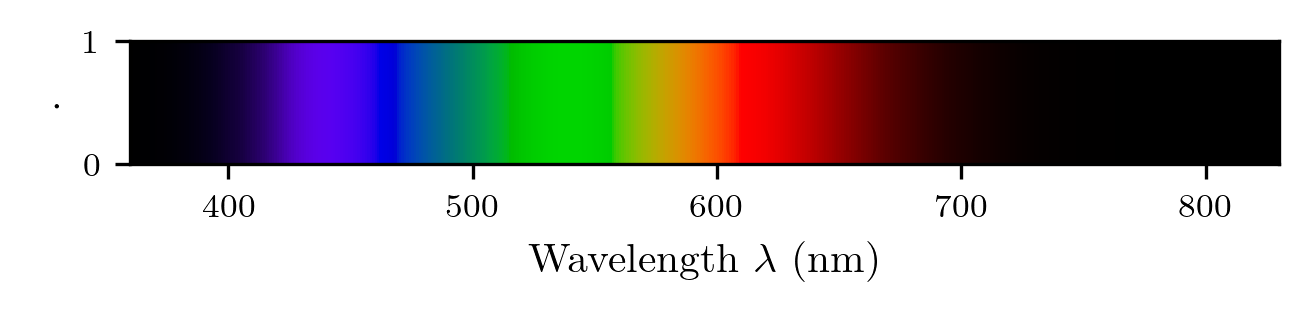
\includegraphics[width=\textwidth]{CIE_visible_spectrum}
        \caption{}
        \label{fig:visual_spectrum}
    \end{subfigure}\\
    %~ %add desired spacing between images, e. g. ~, \quad, \qquad, \hfill etc. 
      %(or a blank line to force the subfigure onto a new line)
    \begin{subfigure}[c]{0.65\textwidth}
        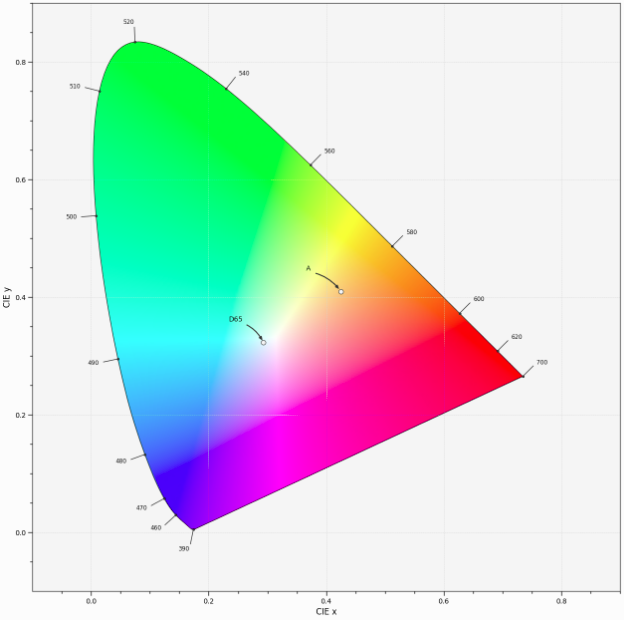
\includegraphics[width=\textwidth]{CIE_chromaticity_diagram}
        \caption{}
        \label{fig:chrom_diagram}
    \end{subfigure} 
                      
    \caption{CIE 1931 2 Degree Standard Observer: visible light spectrum {\small \textsf{\textbf{(a)}}} and chromaticity diagram {\small \textsf{\textbf{(b)}}}.}\label{fig:cie_standard_observer}    
\end{figure}

With the standard primaries it is possible to quantify an object’s colors using a standardized method that takes into account the human eye’s (observer) response to these colors through the \textbf{XYZ color model} (also known as the CIEXYZ color model). In the model $X$, $Y$ and $Z$ are the amount of each primary needed to produce a desired color
\begin{eqnarray} 
 c(\lambda) = (X,Y,Z) \label{eq:XYZ_color}
\end{eqnarray}
where the primary $Y$ is chosen such that its color-matching function exactly matches the luminous-efficiency function for the human eye, i.e., $Y$ measure the luminance of a color \citep{Wright:BookCh2:2007}. Therefore, to define a color in this space, we need to provide the weights for the $X$, $Y$ and $Z$ primaries, for example, $c =xX + yY + zZ$, where 
\begin{gather} 
	x = \frac{X}{X+Y+Z} \nonumber \\ 
	y = \frac{Y}{X+Y+Z} \label{eq:xyz_color_coords} \\ 
	z = \frac{Z}{X+Y+Z} \nonumber 
\end{gather}

Under this representation, we can ignore the dimension of the luminance by the normalizacion of the primaries with the total light intensity; $x+y+z=1$. This allow to show all visibles colors of the spectrum in a diagram. Figure \ref{fig:chrom_diagram} shows such a diagram known as the CIE 1931 2 degree standard observer chromaticity chart. The $x$ and $y$ axis of the diagram give the normalised amounts of the $X$ and $Y$ primaries for a particular color, and hence $z = 1 - x - y$ gives the amount of the $Z$ primary required. The diagram reveals that large $x$ values correspond to red or orange hues, large values of $y$ correspond to green and, large $z$ values correspond to blue, violet or purple hues. Chromaticity depends on dominant wavelength and saturation, and is independent of luminous energy. Colors with the same chromaticity but different luminance, all map to the same point within this region. Moreover, the boundary of the chart represents maximum saturation for the visible colors, and the diagram forms the boundary of all perceivable hues \citep{Bull:Book:2014}. 

The CIEXYZ model is a reference which has been uses as a basis for to defining other color spaces, and therefore as a standard basis in image processing for moving from one color space to another. The color gamut that can be created through combinations of any three primary colors (e.g. RGB) can be represented on the chromaticity diagram by a triangle joining the coordinates for the three colors. 
%Images of RGB, HSV, HSL, LAB models?

The \textbf{RGB color model} is one of the most popular models in computer vision and image analysis. This is an additive model coming directly from the three-component theory, this means that three color light beams (their wavelength light spectra) are added together to make a final color \citep{Gonzalez.Woods:Book:2008}. The model consists of three independent planes, represented as a three dimensional vector, one in each of the primary colors: red, green and blue. Therefore, to define a color in this model, we need to specify the proportion of red, green, and blue colors. 

Contrary to the XYZ model, the RGB color space is a device-dependent space, that is, different devices may reproduce or detect the same RGB value differently since the color elements and their response to the individual R, G, and B levels vary according to the manufacturer.

The RGB color space is the most popular color space based on the RGB color model. The set of colors of this color space can be represented geometrically as a cube that maps the red, blue and green dimensions onto the $x$, $y$, $z$ axes of the 3-d Cartesian coordinate system in an Euclidean space. The non-negative values of the $RGB$ triplet $(r,g,b)$ are in the range $[0,1]$, where the origin at the vertex $(0,0,0)$ encodes the color black and the vertex $(1,1,1)$ encodes the color white. 

The \textbf{HSV color model} and the \textbf{HSL color model} are cylindrical color models that remaps the RGB primary colors into dimensions that are easier for humans to understand. These two colos models share two of their three dimensions, the hue and the saturation. The third dimension of the HSV model is the value while the HSL model has a lightness dimension. Below is a more detailed description of these dimensions.

\begin{itemize}
	\item Hue specifies the angle of the color on the RGB color circle. A $0^\circ$ hue results in red, $120^\circ$ results in green, and $240^\circ$ results in blue.
	\item Saturation or colorfulness controls the amount of color used. One particular thing about the saturation between the two cylindrical color spaces is that even though the saturation dimension theoretically is similar between them (controlling how much pure color is used), the resulting saturation scales differ between the models caused by the brightness to lightness remapping (see diferences between saturation image channels in figure \ref{fig:color_image_representations}). Therefore, for the HSV model a color with 100\% saturation will be the purest color possible, while 0\% saturation yields grayscale. On the other hand, to obtain the purest color in the HSL model we need 50\% lightness.
	\item Value controls the brightness of the color. A color with 0\% value is pure black while a color with 100\% value has no black mixed into the color. Because this dimension is often referred to as brightness, the HSV color model is sometimes called HSB.
	\item Lightness controls the luminosity of the color. This dimension is different from the HSV value dimension in that the purest color is positioned midway between black and white ends of the scale. A color with 0\% lightness is black, 50\% is the purest color possible, and 100\% is white.
\end{itemize}

It is important to note that the three dimensions of the HSV/HSL color models are interdependent. If the value/lightness dimension of a color is set to 0\%, the amount of hue and saturation does not matter as the color will be black. Likewise, if the saturation of a color is set to 0\%, the hue does not matter as there is no color used.

Unlike the RGB color space, the HSV/HSL triplet values $(h,s,v)$/$(h,s,l)$c annot be represented in a 3-d Euclidean space. The circular nature of the hue forces the first dimension to be in an angular space between $0^\circ$ and $360^\circ$, while the remaining two dimensions inhabit a linear space with values between 0 and 1. Consequetly, the HSV color space is best visualized as 3-d cone and the HSL color space as a 3-d bicone. 

The \textbf{LAB color model} (also referred as CIEL*a*b* or CIELAB) is a result of the opponent-process theory of human perception. In it, color is also expressed with three values. Channel L represents the perceptual luminance wjereas channels A and B represent the scale from red to green and from yellow to blue respectively, which is consistent with the two opponent color pairs that humans cannot perceive simultaneously. 

The color space from the LAB model was born with the intention of being a perceptually uniform space, that is, a space where a given numerical change corresponds to the same perception of change in color. As a non-linear transformation of the XYZ color space, the LAB color space is a device-independent space. This implies that its gamut is related to the CIE standard observer model, and therefore, it is impossible to generate a visual representation that displays all the colors of its gamut. The LAB space coordinates are given by the triplet $(l,a,b)$. The first valuer represent the luminance L and it may take values from $0$ to $100$, where 0 points to black and $100$ indicates (diffuse) white. The remaining two coordinates are technically unbounded, though it is commonly mapped to the range $[-128, 127]$. Negative values indicate green and positive values red for channel A, while negative values indicate yellow and positive values blue for channel B. 

This color space offers some advantages over the spaces described above, especially in the area of image processing. The fact that this space was constructed to approximate human color vision makes it useful for calculating differences between two neighboring colors with high precision. However, this color model contains colors that are not physically representable by the devices, and a bad color quantization (bits per channel) can generate significant errors.

\begin{figure}[!ht]
    \begin{subfigure}[t]{\dimexpr0.3\textwidth+20pt\relax}
    	\makebox[20pt]{\raisebox{35pt}{ \rotatebox[origin=c]{90} {\small \textsf{\textbf{Input image}}} }}%
    	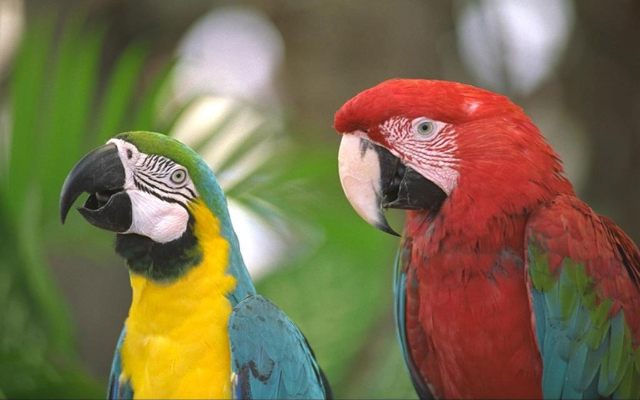
\includegraphics[width=\dimexpr\linewidth-20pt\relax]{araras}
    \end{subfigure} \\    
     
    \begin{subfigure}[t]{\dimexpr0.3\textwidth+20pt\relax}
    	\makebox[20pt]{\raisebox{35pt}{ \rotatebox[origin=c]{90} {\small \textsf{\textbf{RGB channels}}} }}%
    	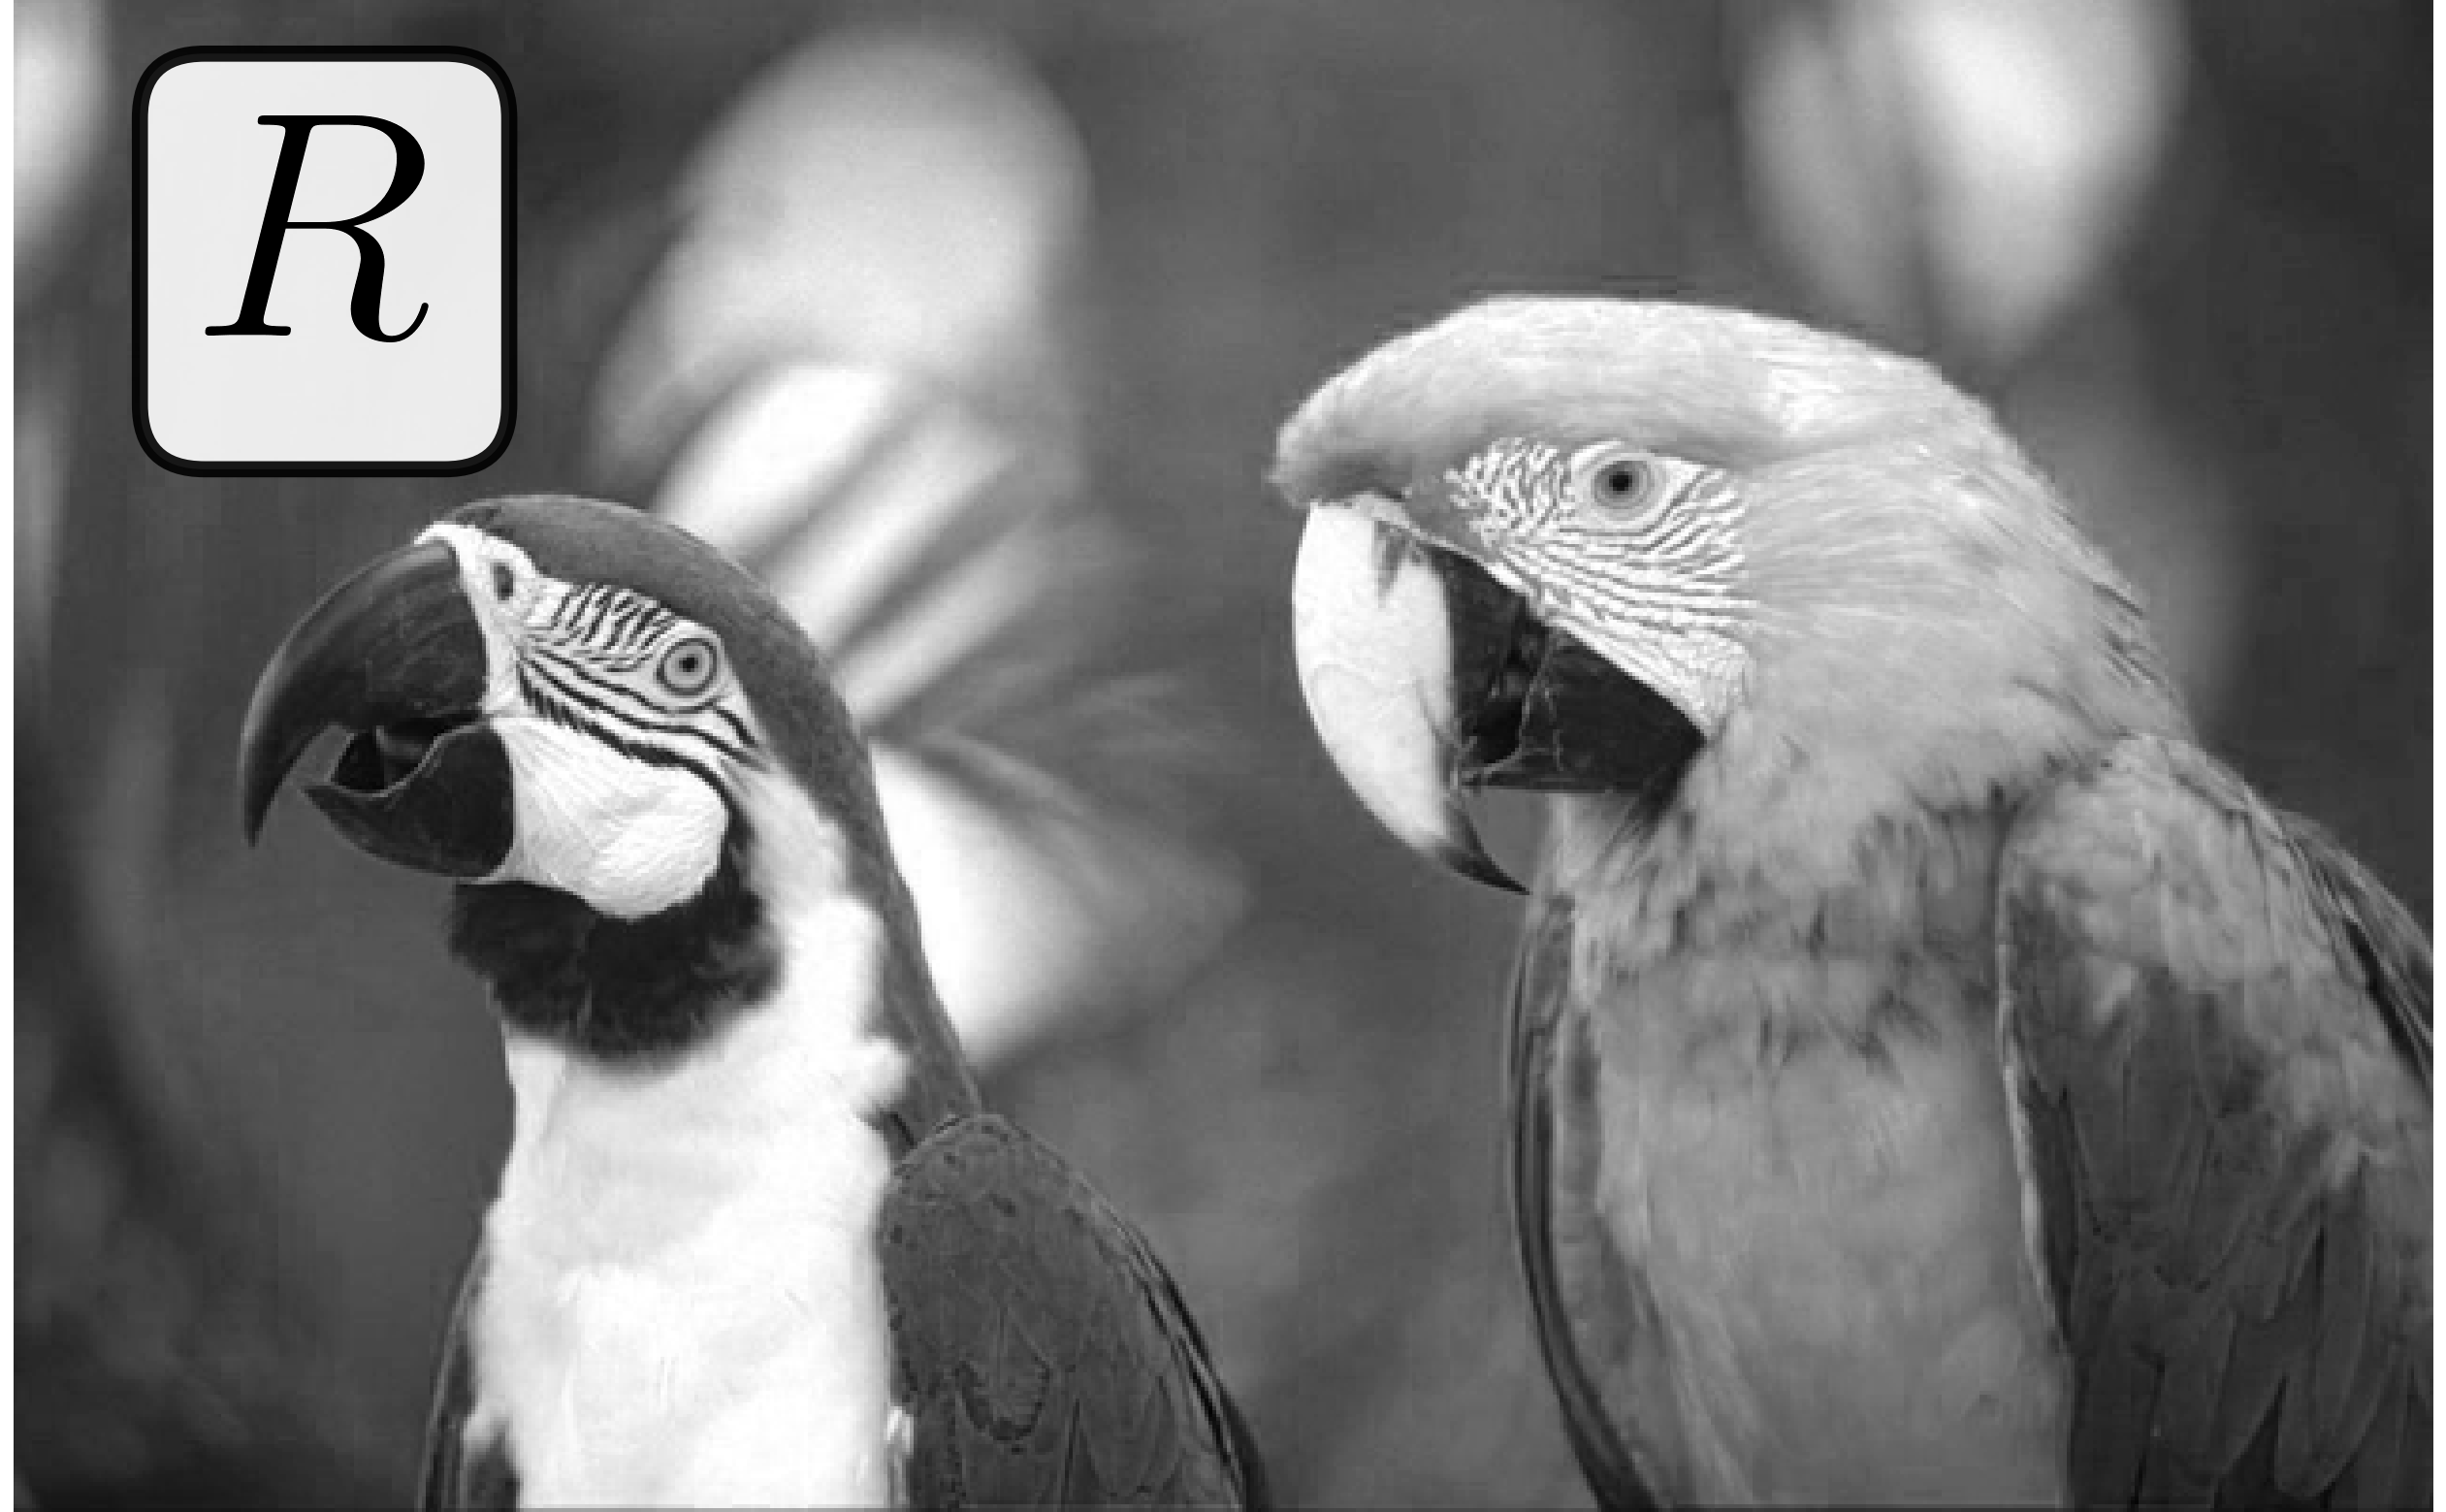
\includegraphics[width=\dimexpr\linewidth-20pt\relax]{araras_R_RGB}
    \end{subfigure}      
    ~ %add desired spacing between images, e. g. ~, \quad, \qquad, \hfill etc. 
      %(or a blank line to force the subfigure onto a new line)
    \begin{subfigure}[b]{0.3\textwidth}
        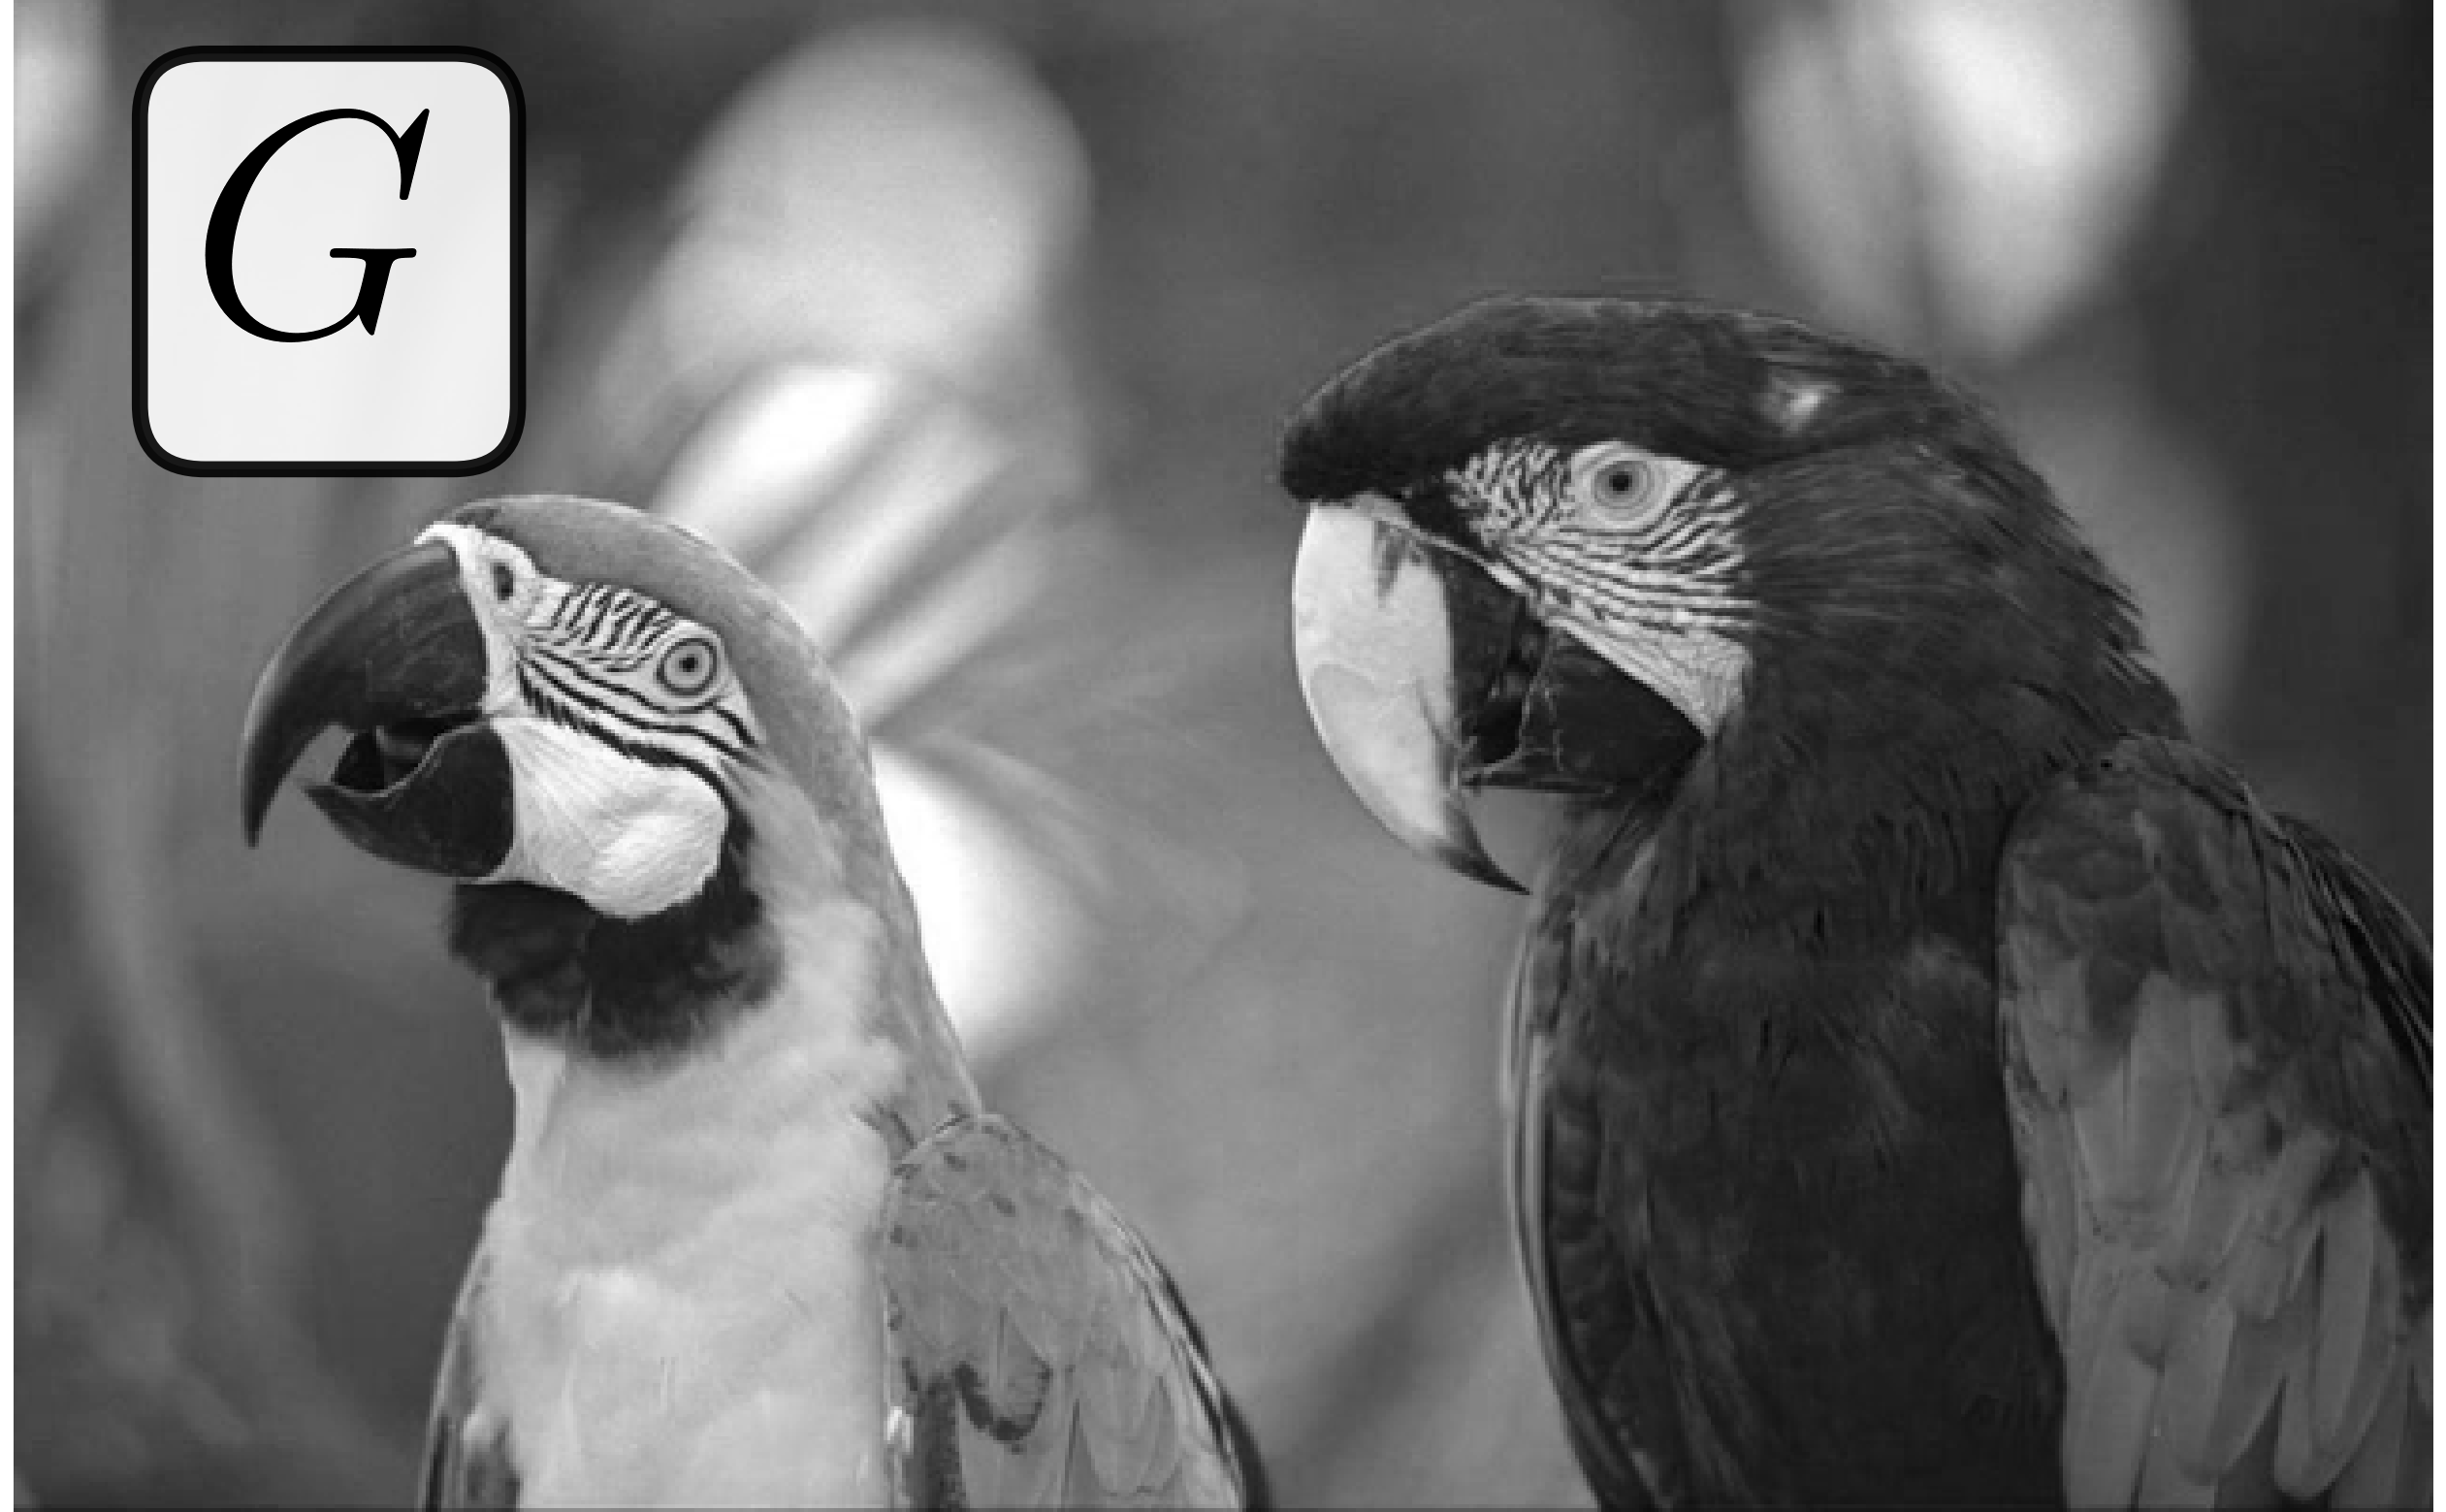
\includegraphics[width=\textwidth]{araras_G_RGB}
    \end{subfigure}
    ~ %add desired spacing between images, e. g. ~, \quad, \qquad, \hfill etc. 
      %(or a blank line to force the subfigure onto a new line)
    \begin{subfigure}[b]{0.3\textwidth}
        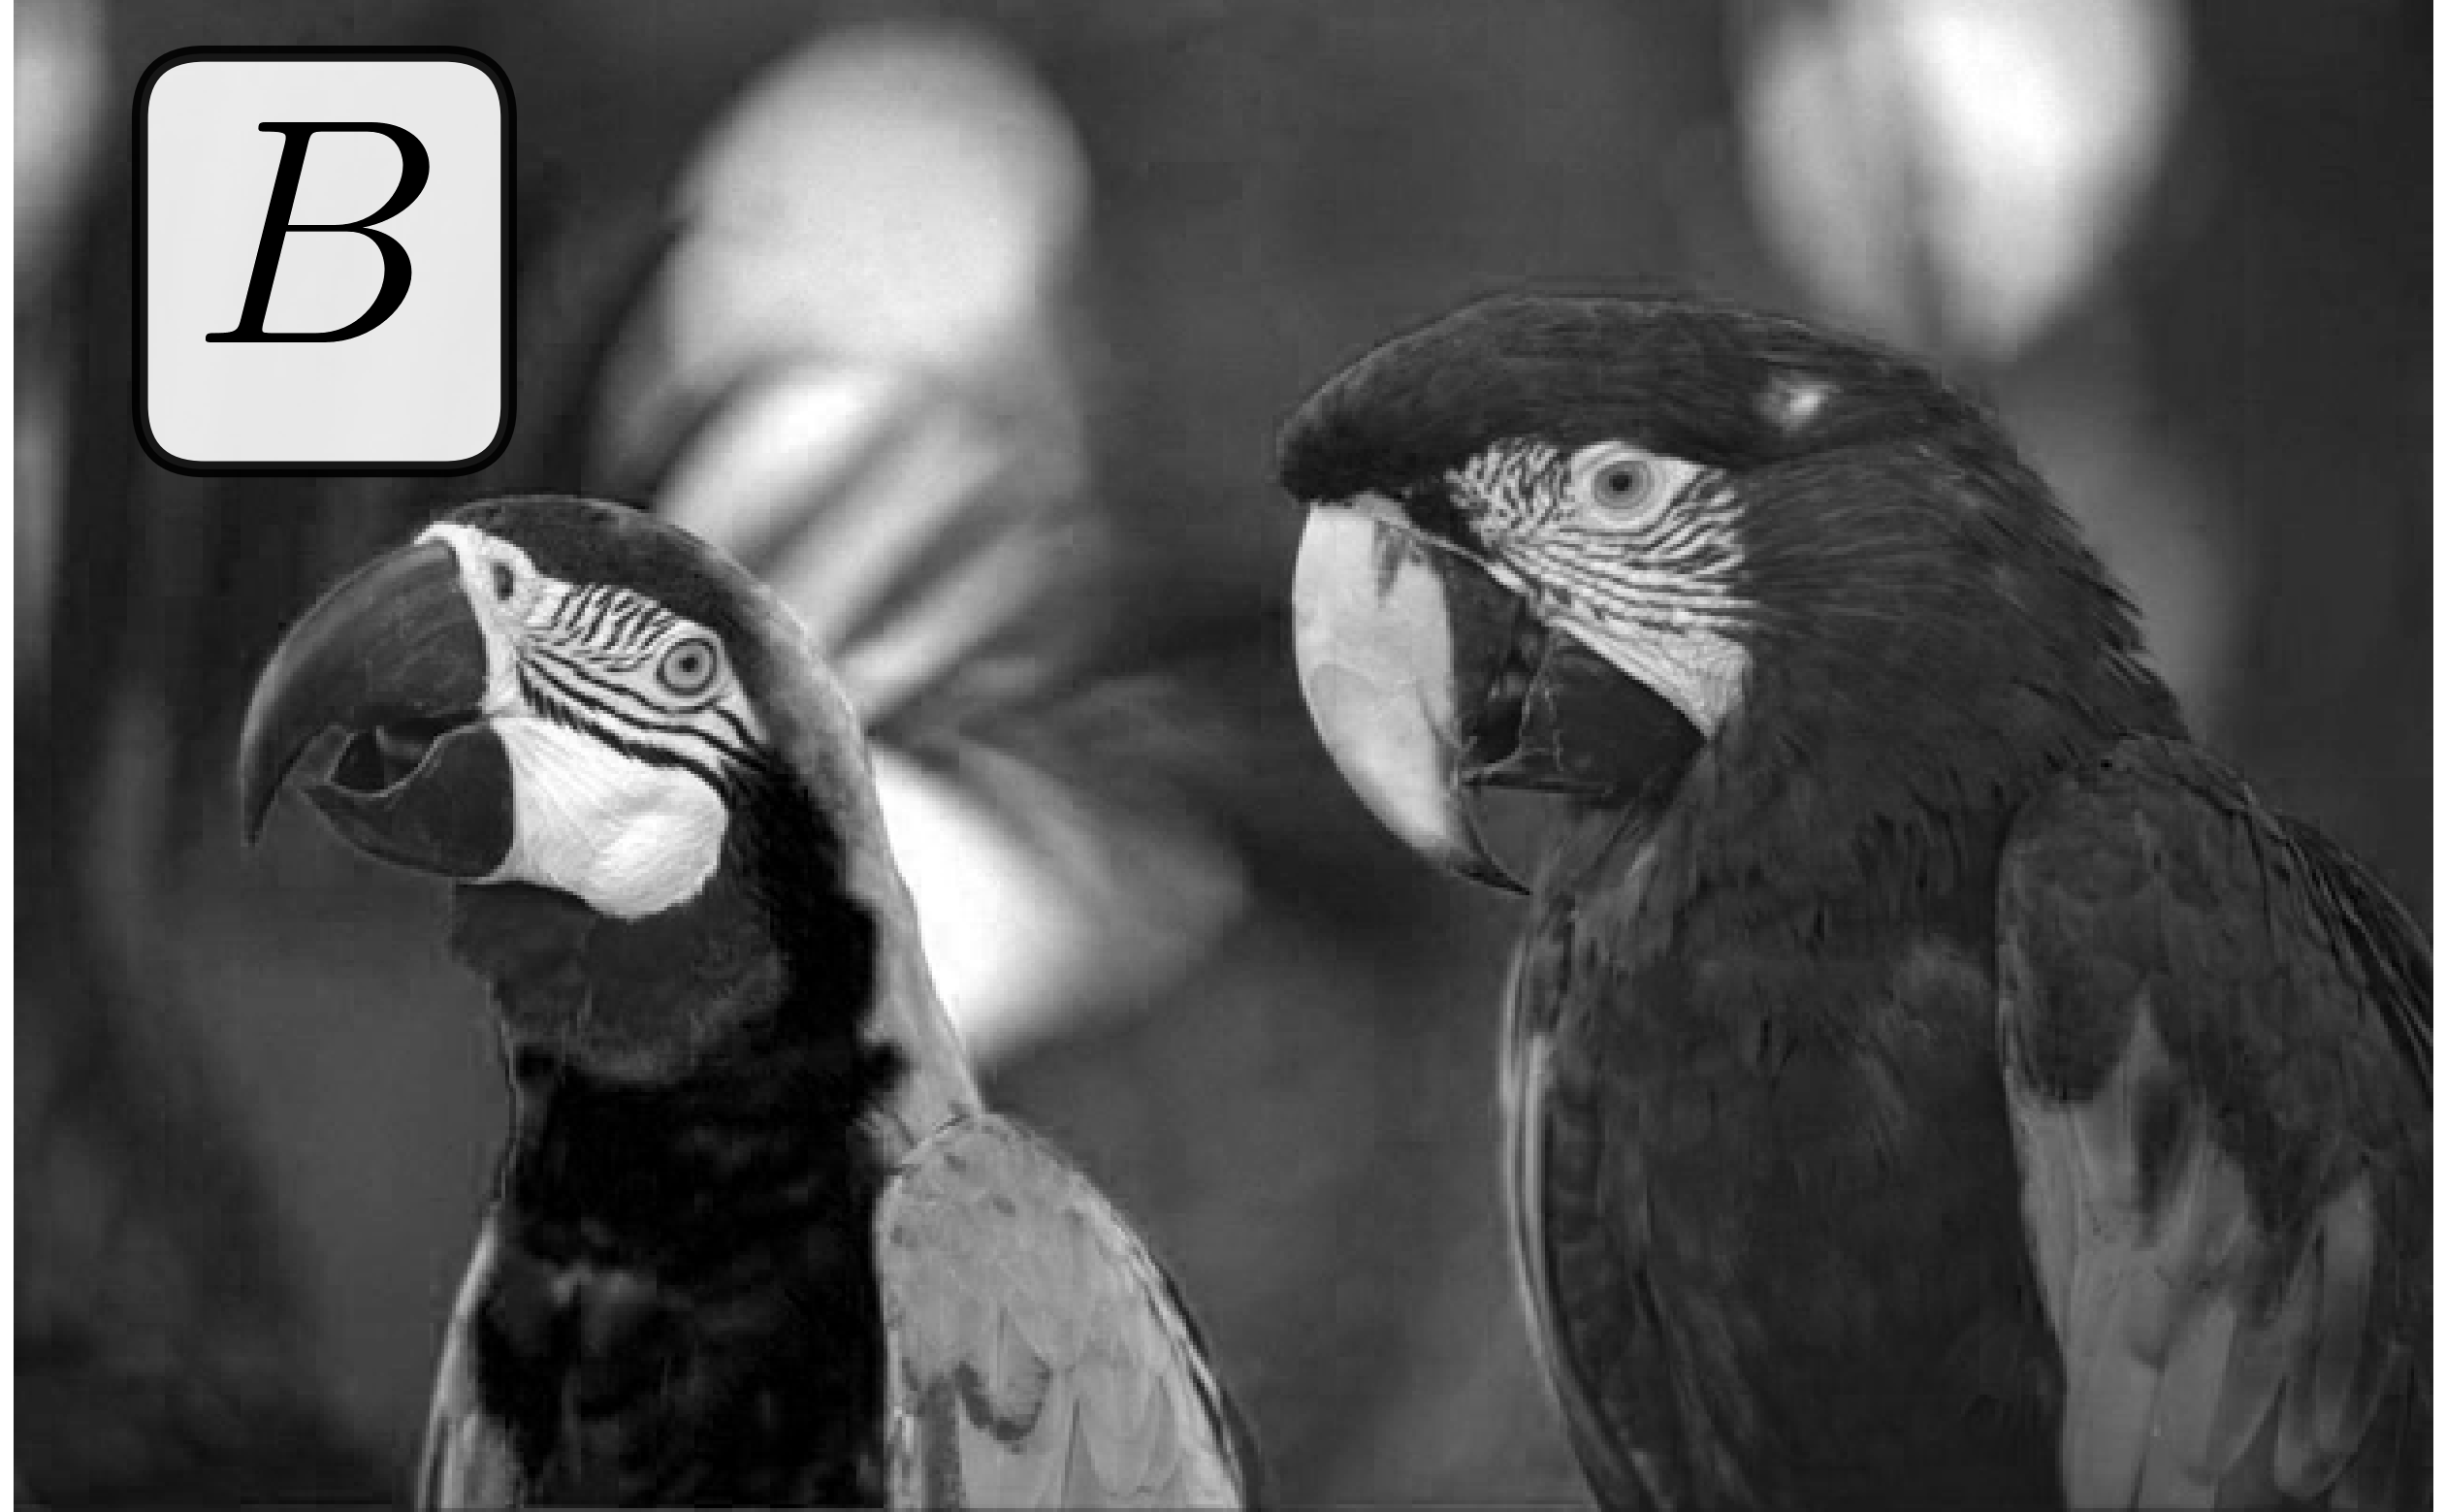
\includegraphics[width=\textwidth]{araras_B_RGB}
    \end{subfigure} \vspace{5pt}      
    
    \begin{subfigure}[t]{\dimexpr0.3\textwidth+20pt\relax}
    	\makebox[20pt]{\raisebox{35pt}{ \rotatebox[origin=c]{90} {\small \textsf{\textbf{HSV channels}}} }}%
    	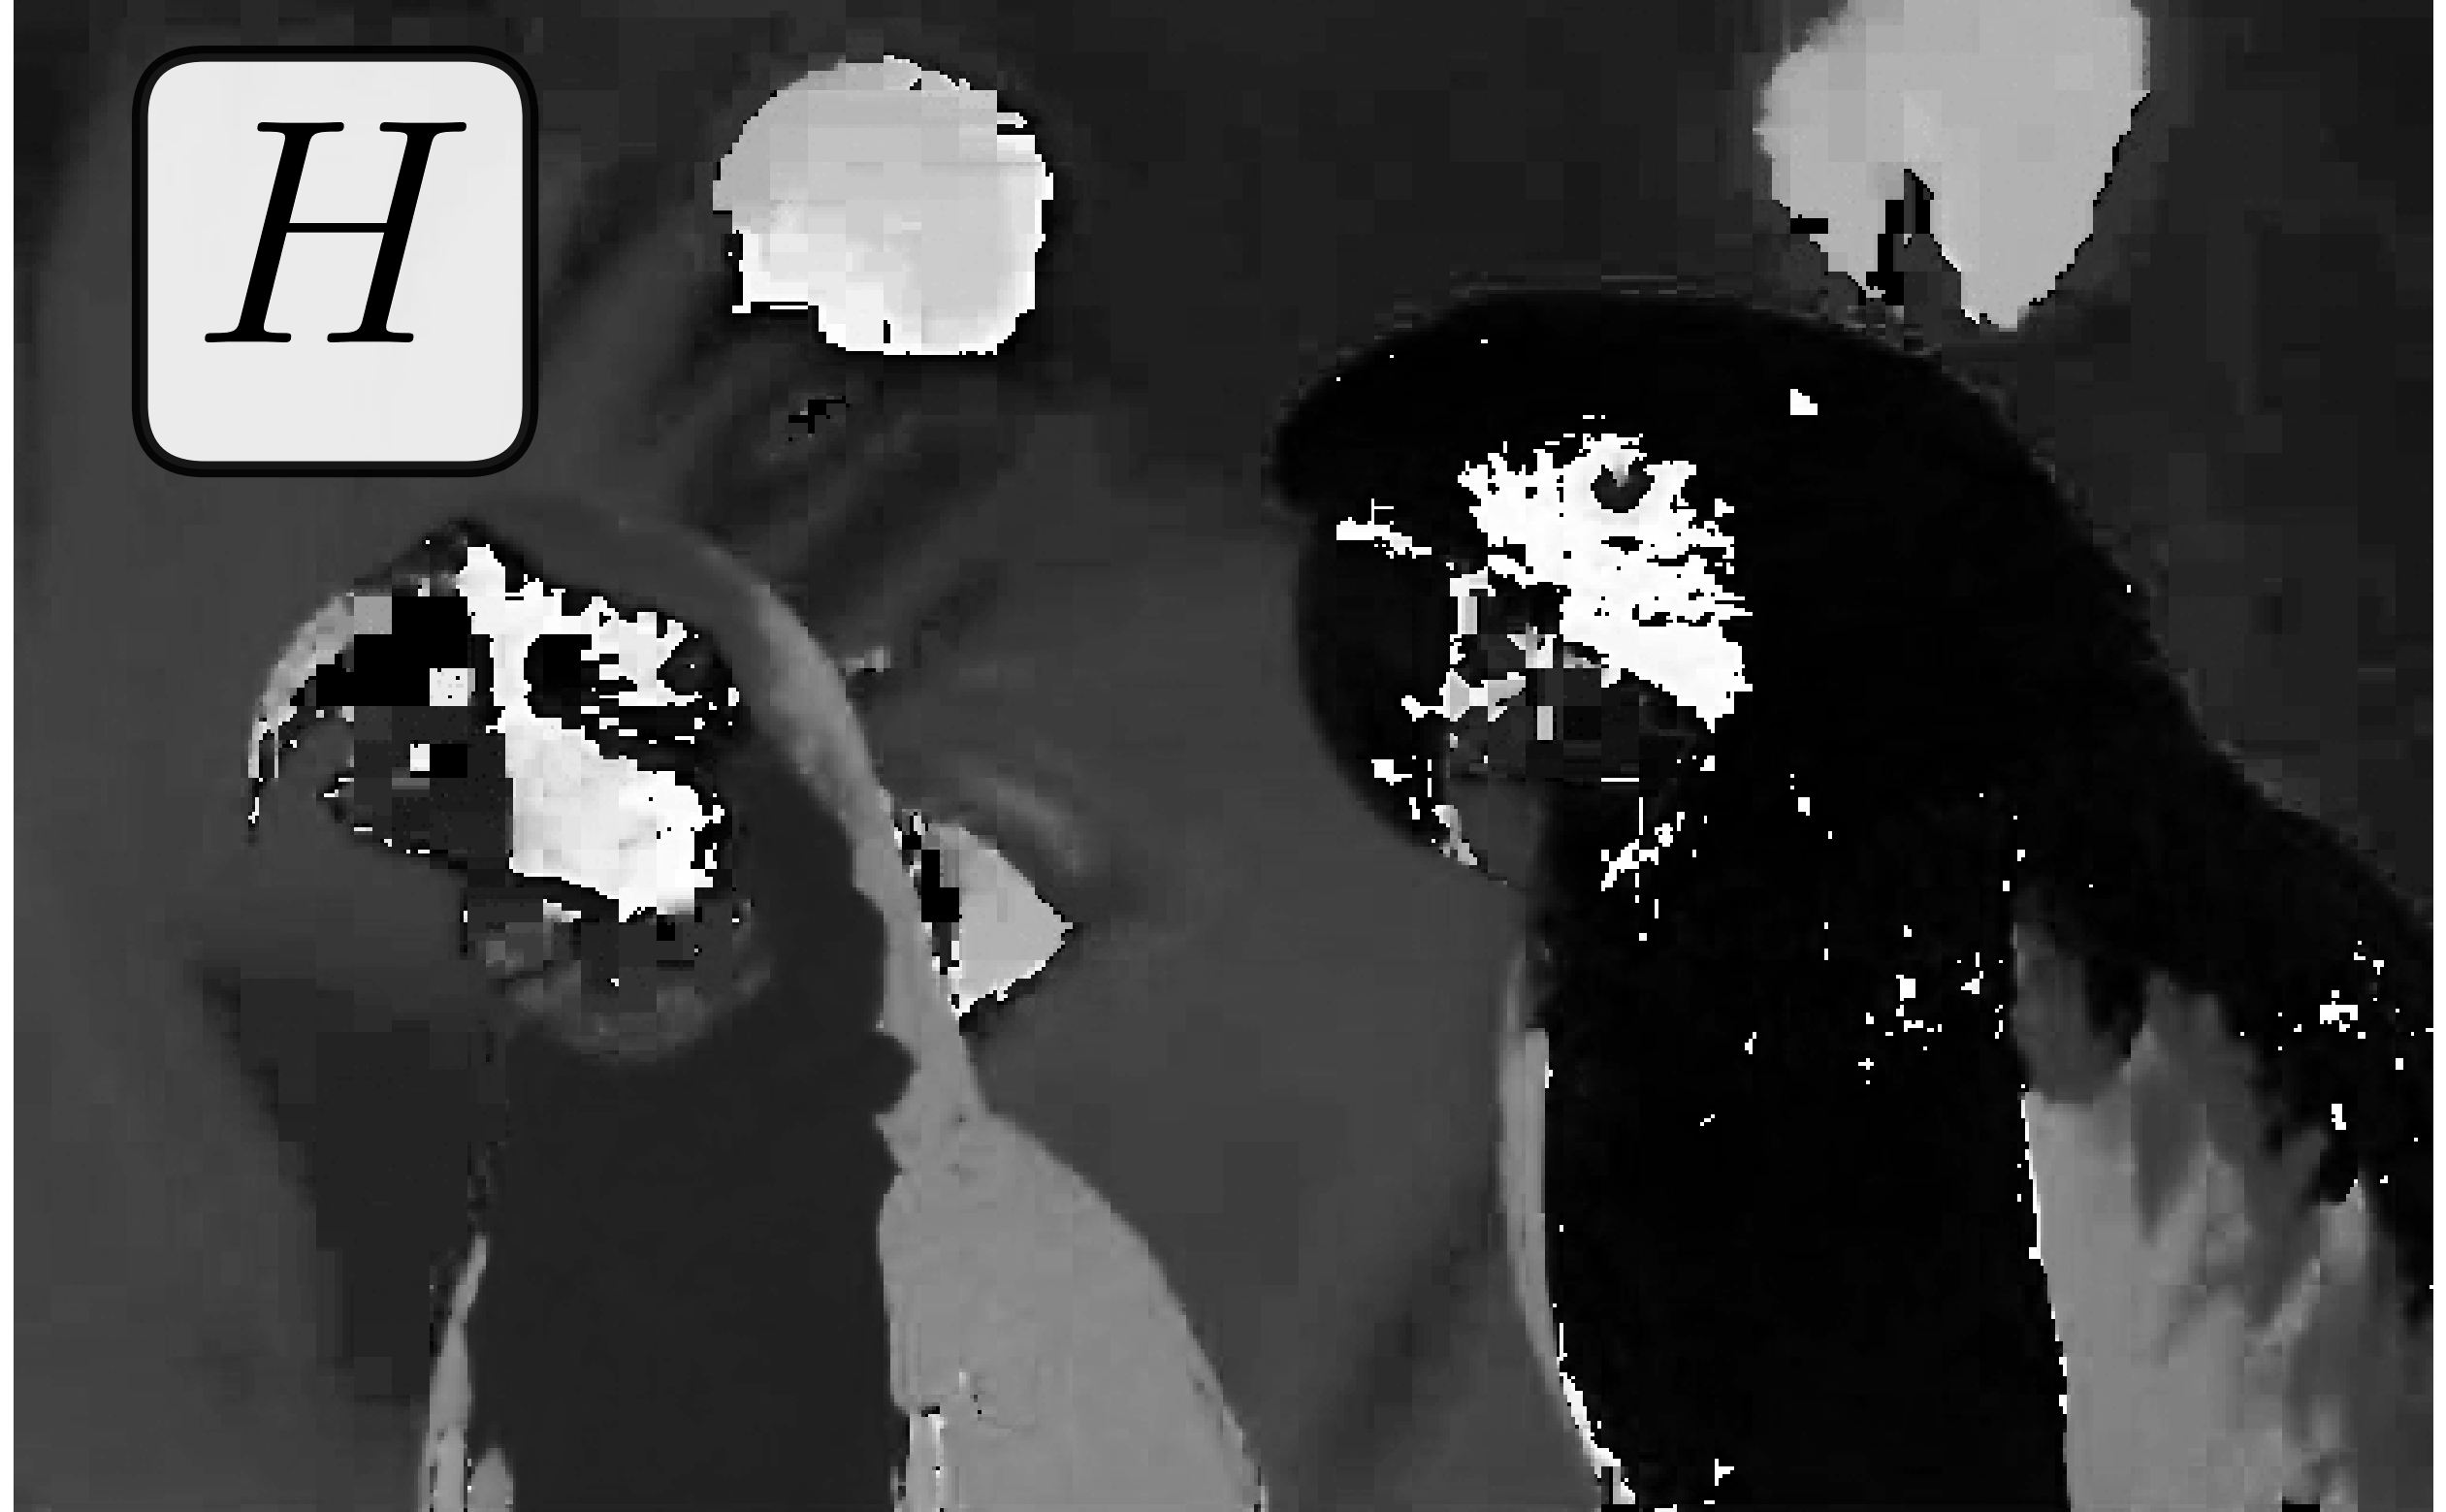
\includegraphics[width=\dimexpr\linewidth-20pt\relax]{araras_H_HSV}
    \end{subfigure}     
    ~ %add desired spacing between images, e. g. ~, \quad, \qquad, \hfill etc. 
      %(or a blank line to force the subfigure onto a new line)
    \begin{subfigure}[b]{0.3\textwidth}
        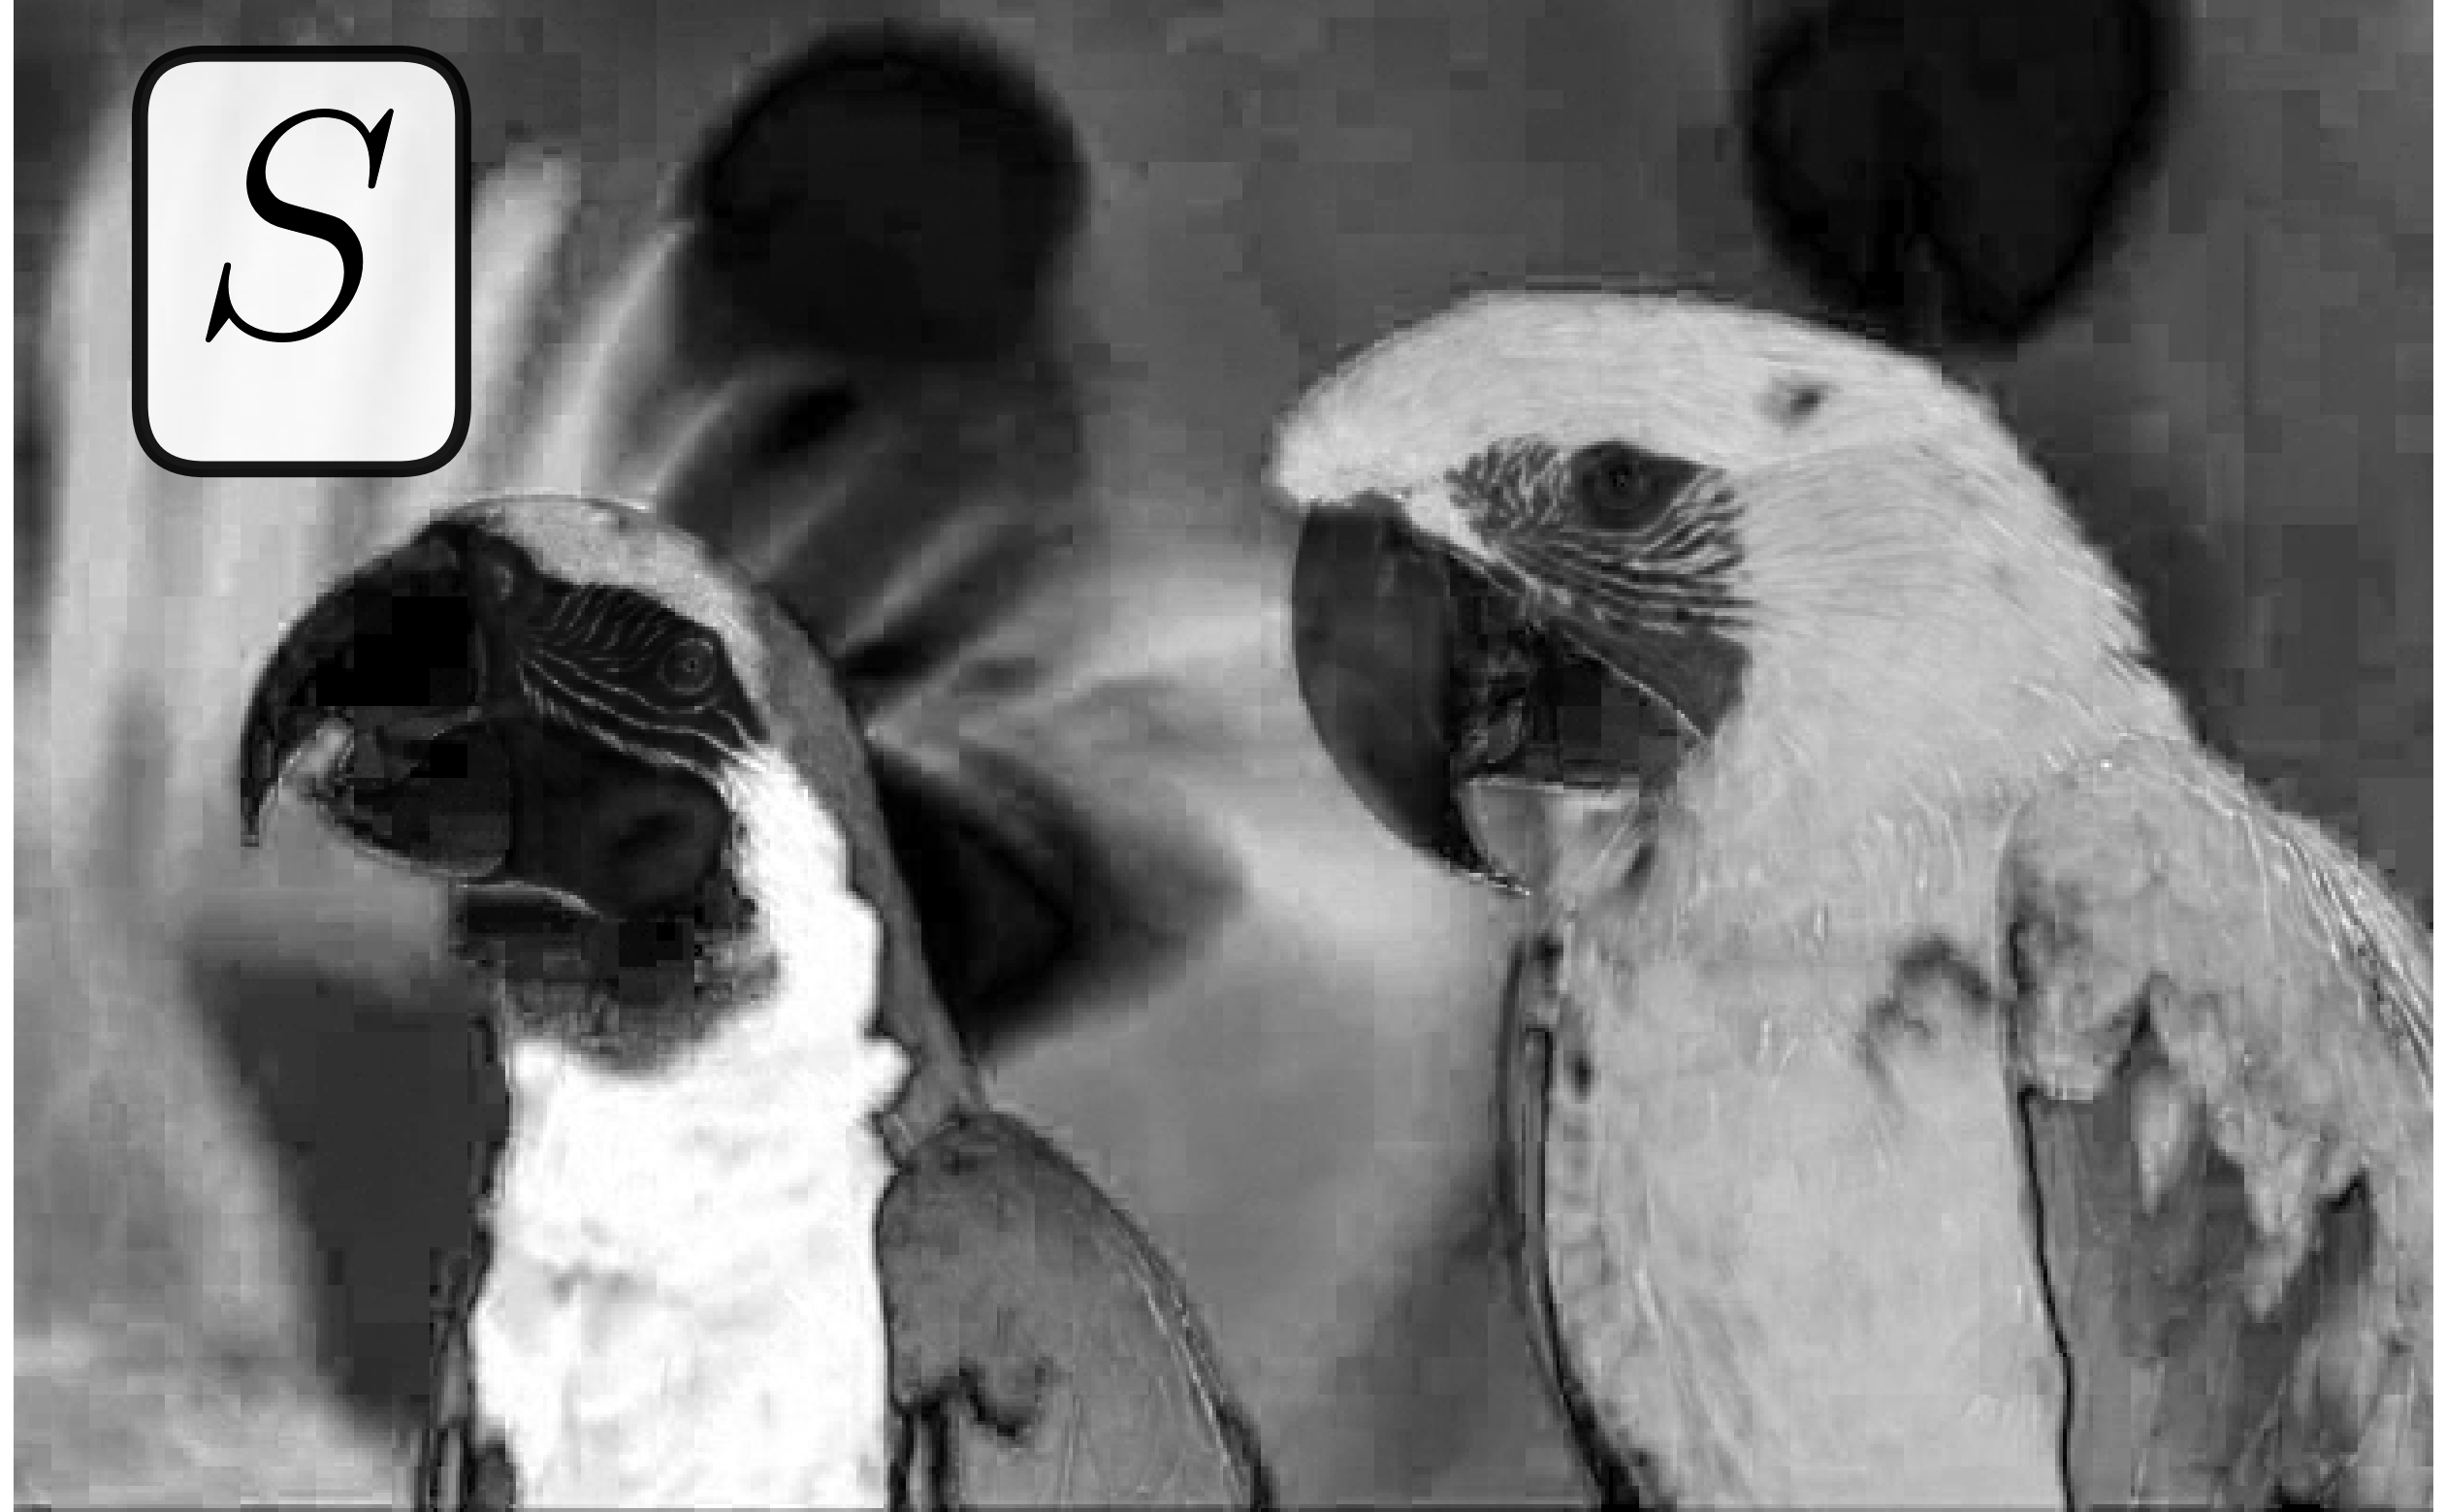
\includegraphics[width=\textwidth]{araras_S_HSV}
    \end{subfigure}
    ~ %add desired spacing between images, e. g. ~, \quad, \qquad, \hfill etc. 
      %(or a blank line to force the subfigure onto a new line)
    \begin{subfigure}[b]{0.3\textwidth}
        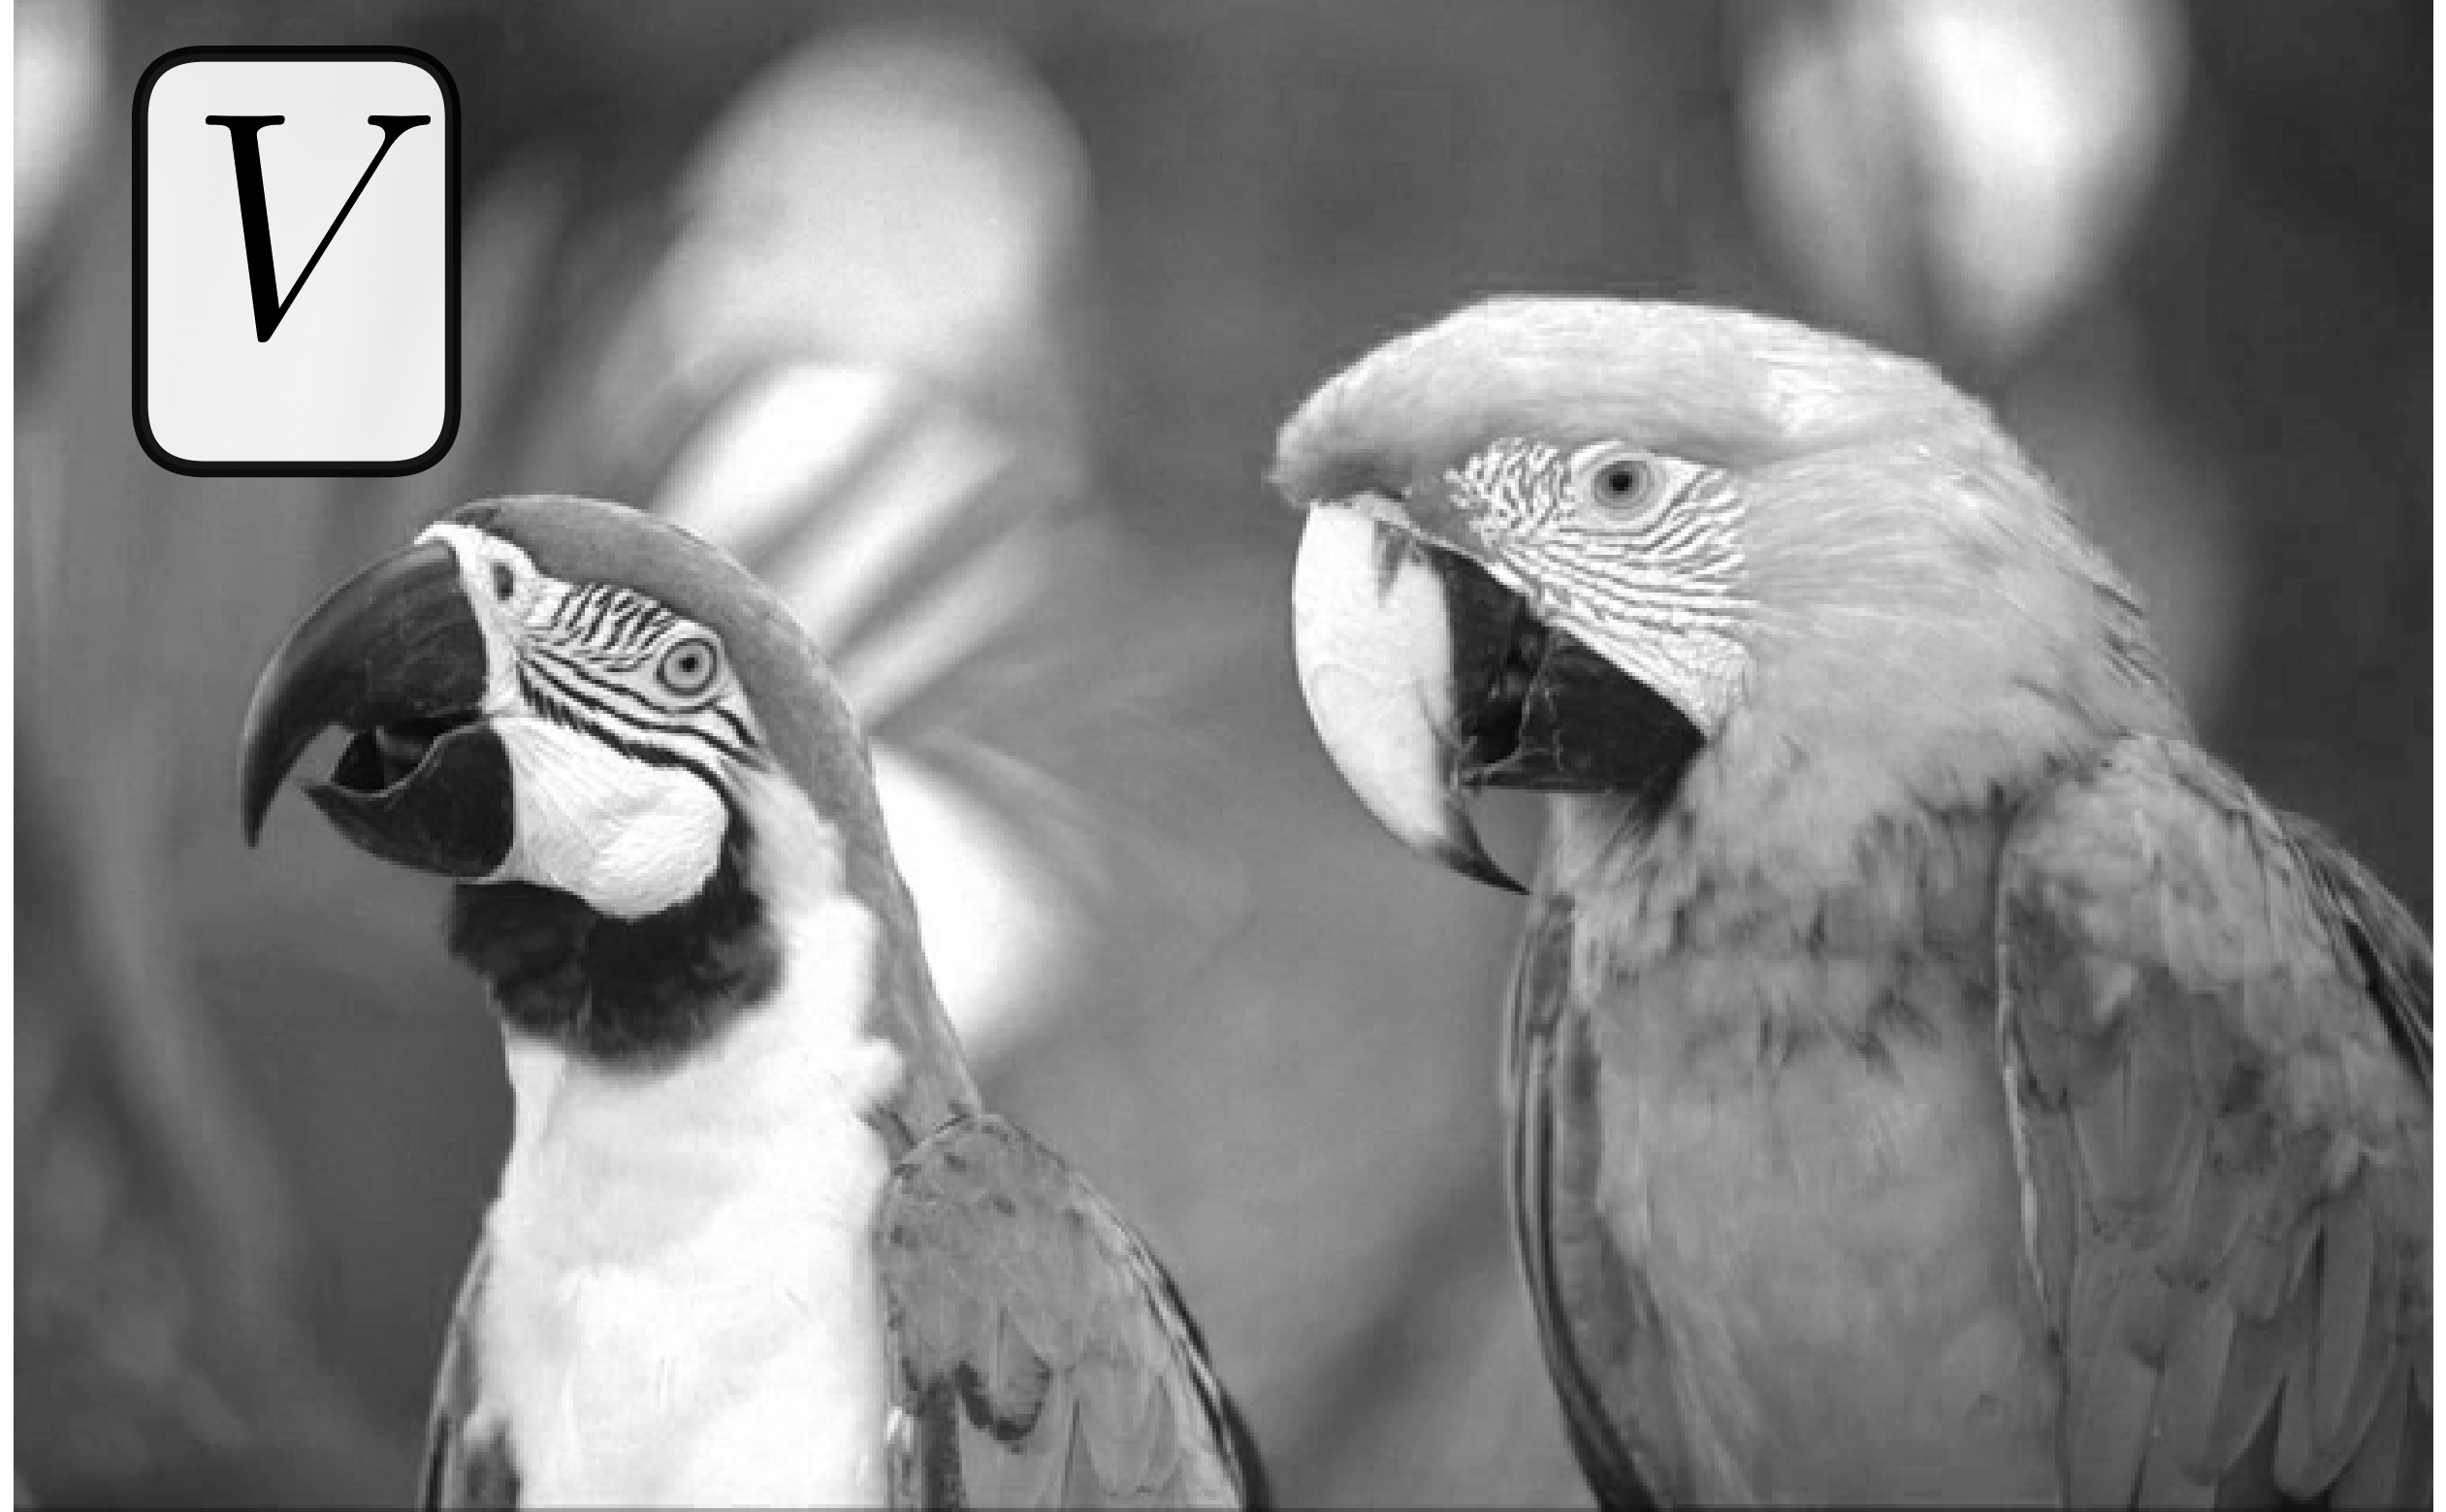
\includegraphics[width=\textwidth]{araras_V_HSV}
    \end{subfigure} \vspace{5pt} 
    
    \begin{subfigure}[t]{\dimexpr0.3\textwidth+20pt\relax}
    	\makebox[20pt]{\raisebox{35pt}{ \rotatebox[origin=c]{90} {\small \textsf{\textbf{HSL channels}}} }}%
    	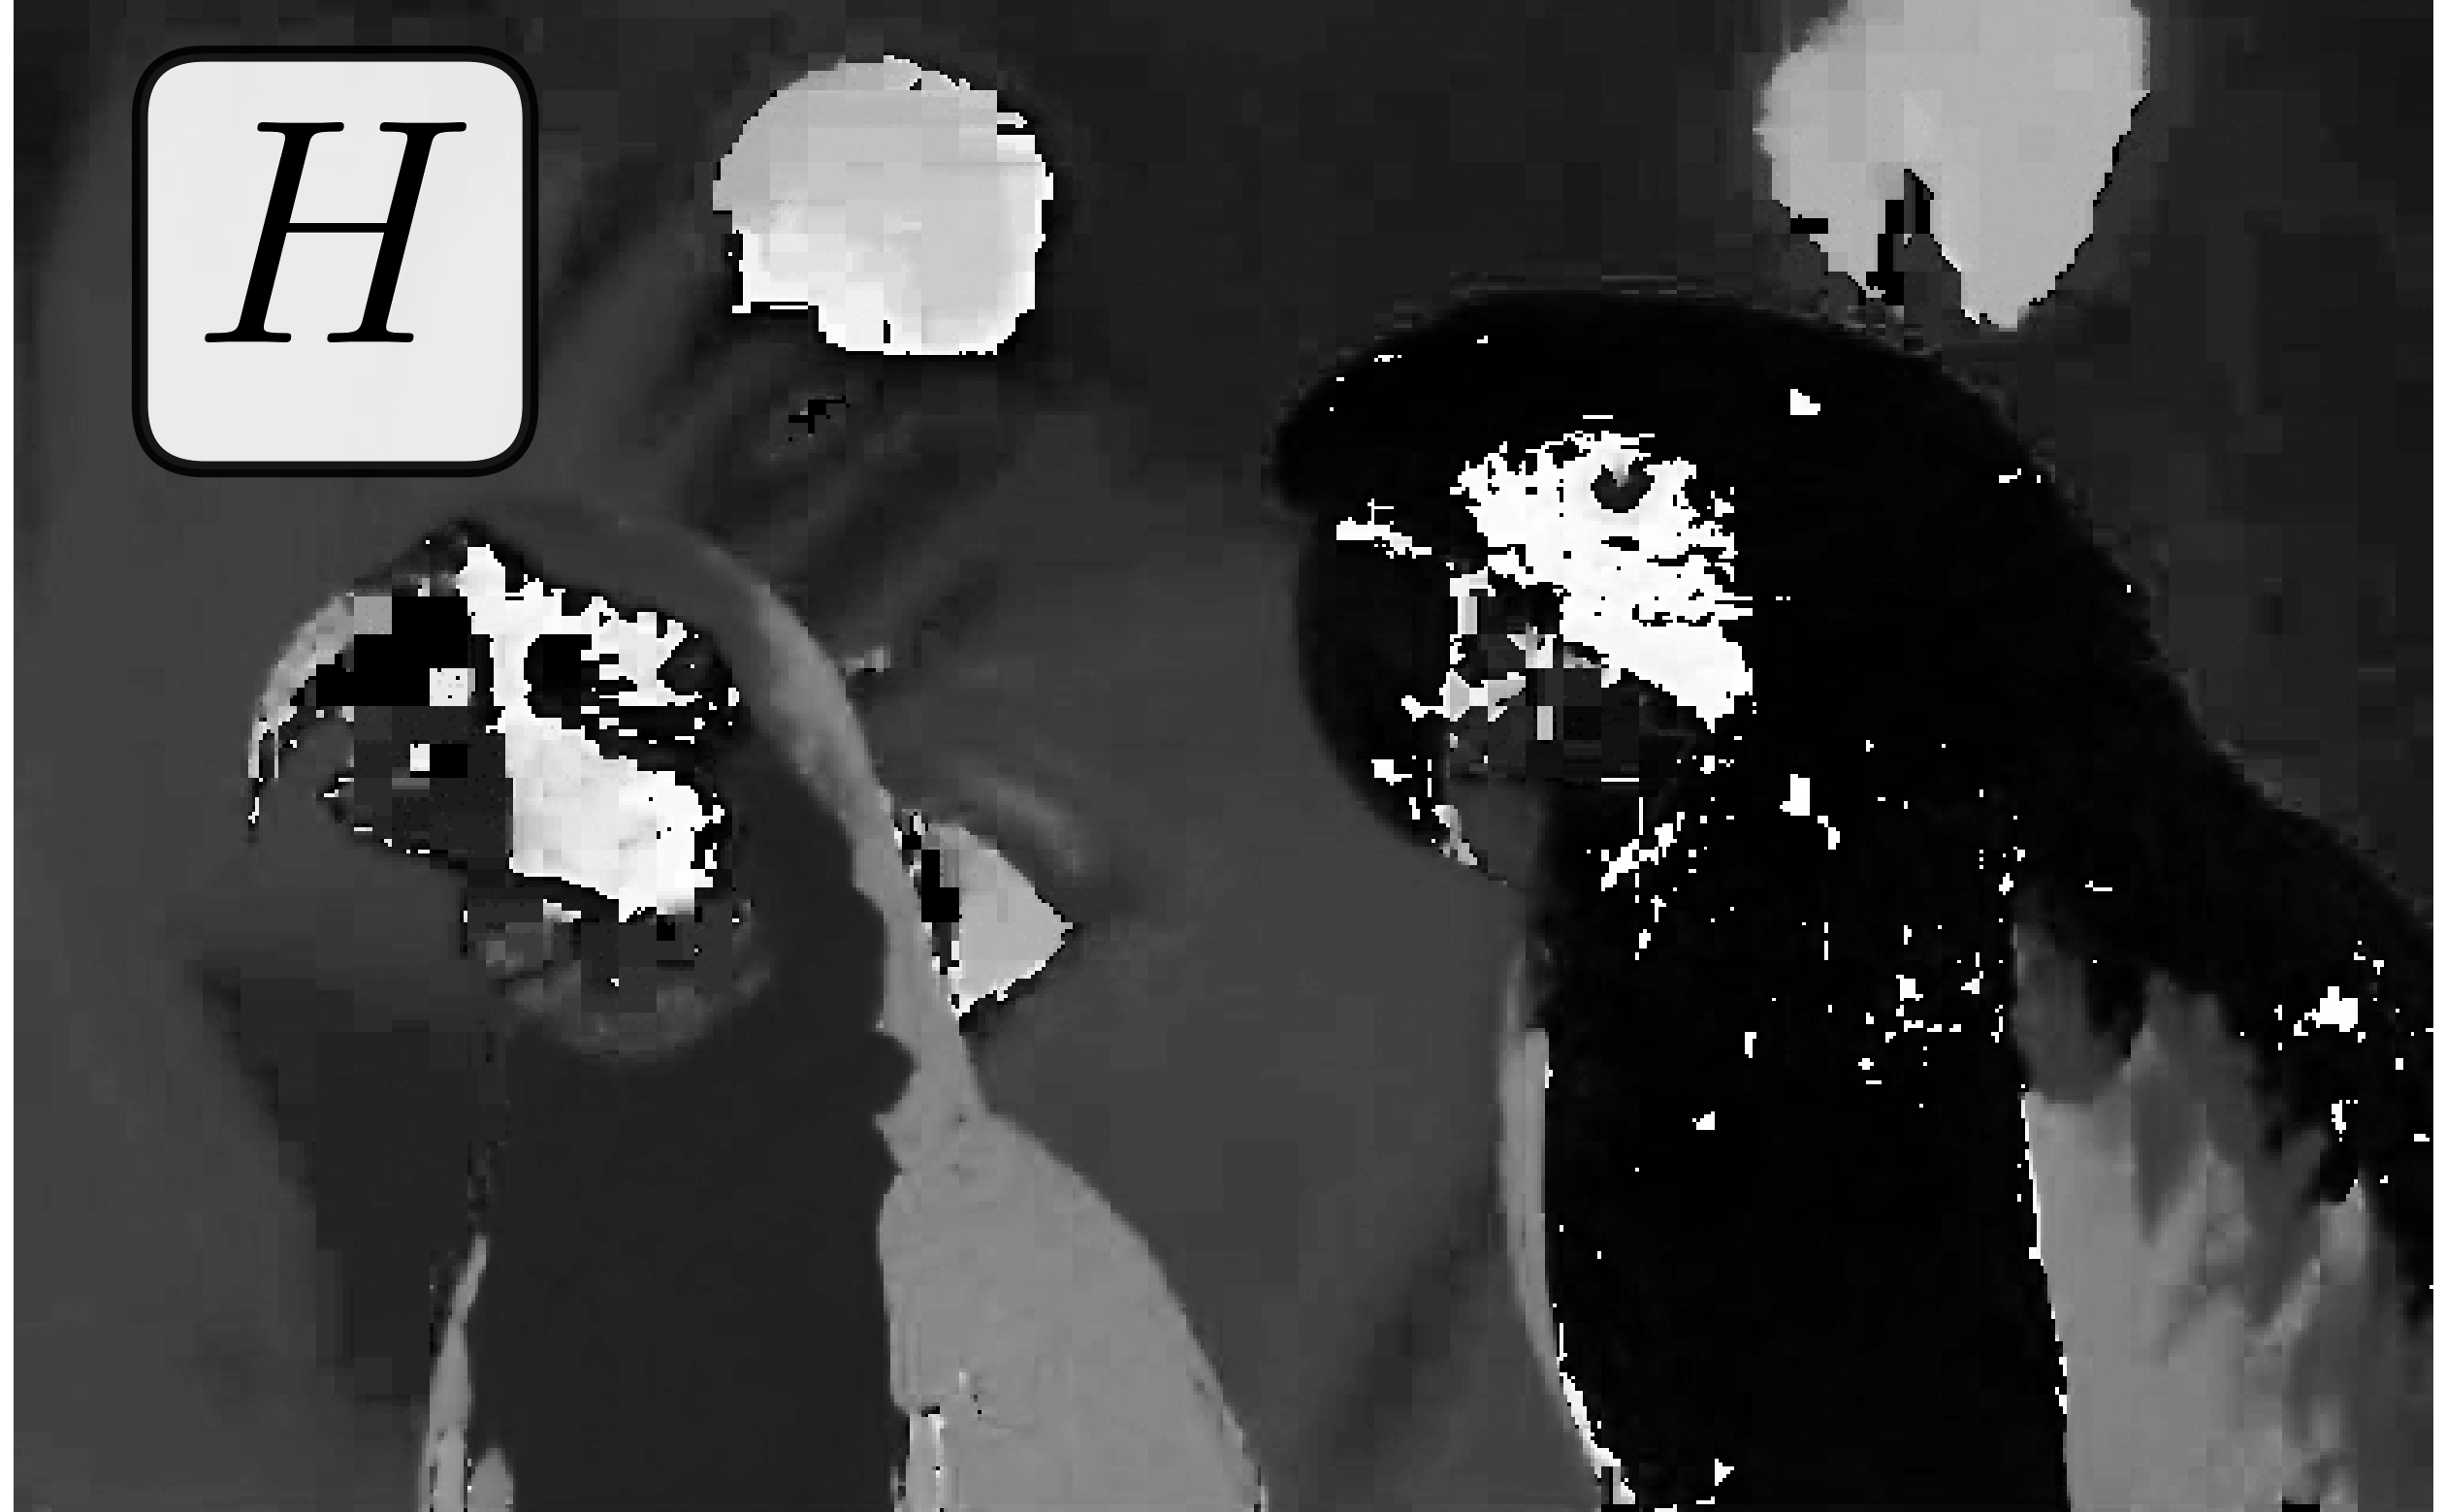
\includegraphics[width=\dimexpr\linewidth-20pt\relax]{araras_H_HLS}
    \end{subfigure}     
    ~ %add desired spacing between images, e. g. ~, \quad, \qquad, \hfill etc. 
      %(or a blank line to force the subfigure onto a new line)
    \begin{subfigure}[b]{0.3\textwidth}
        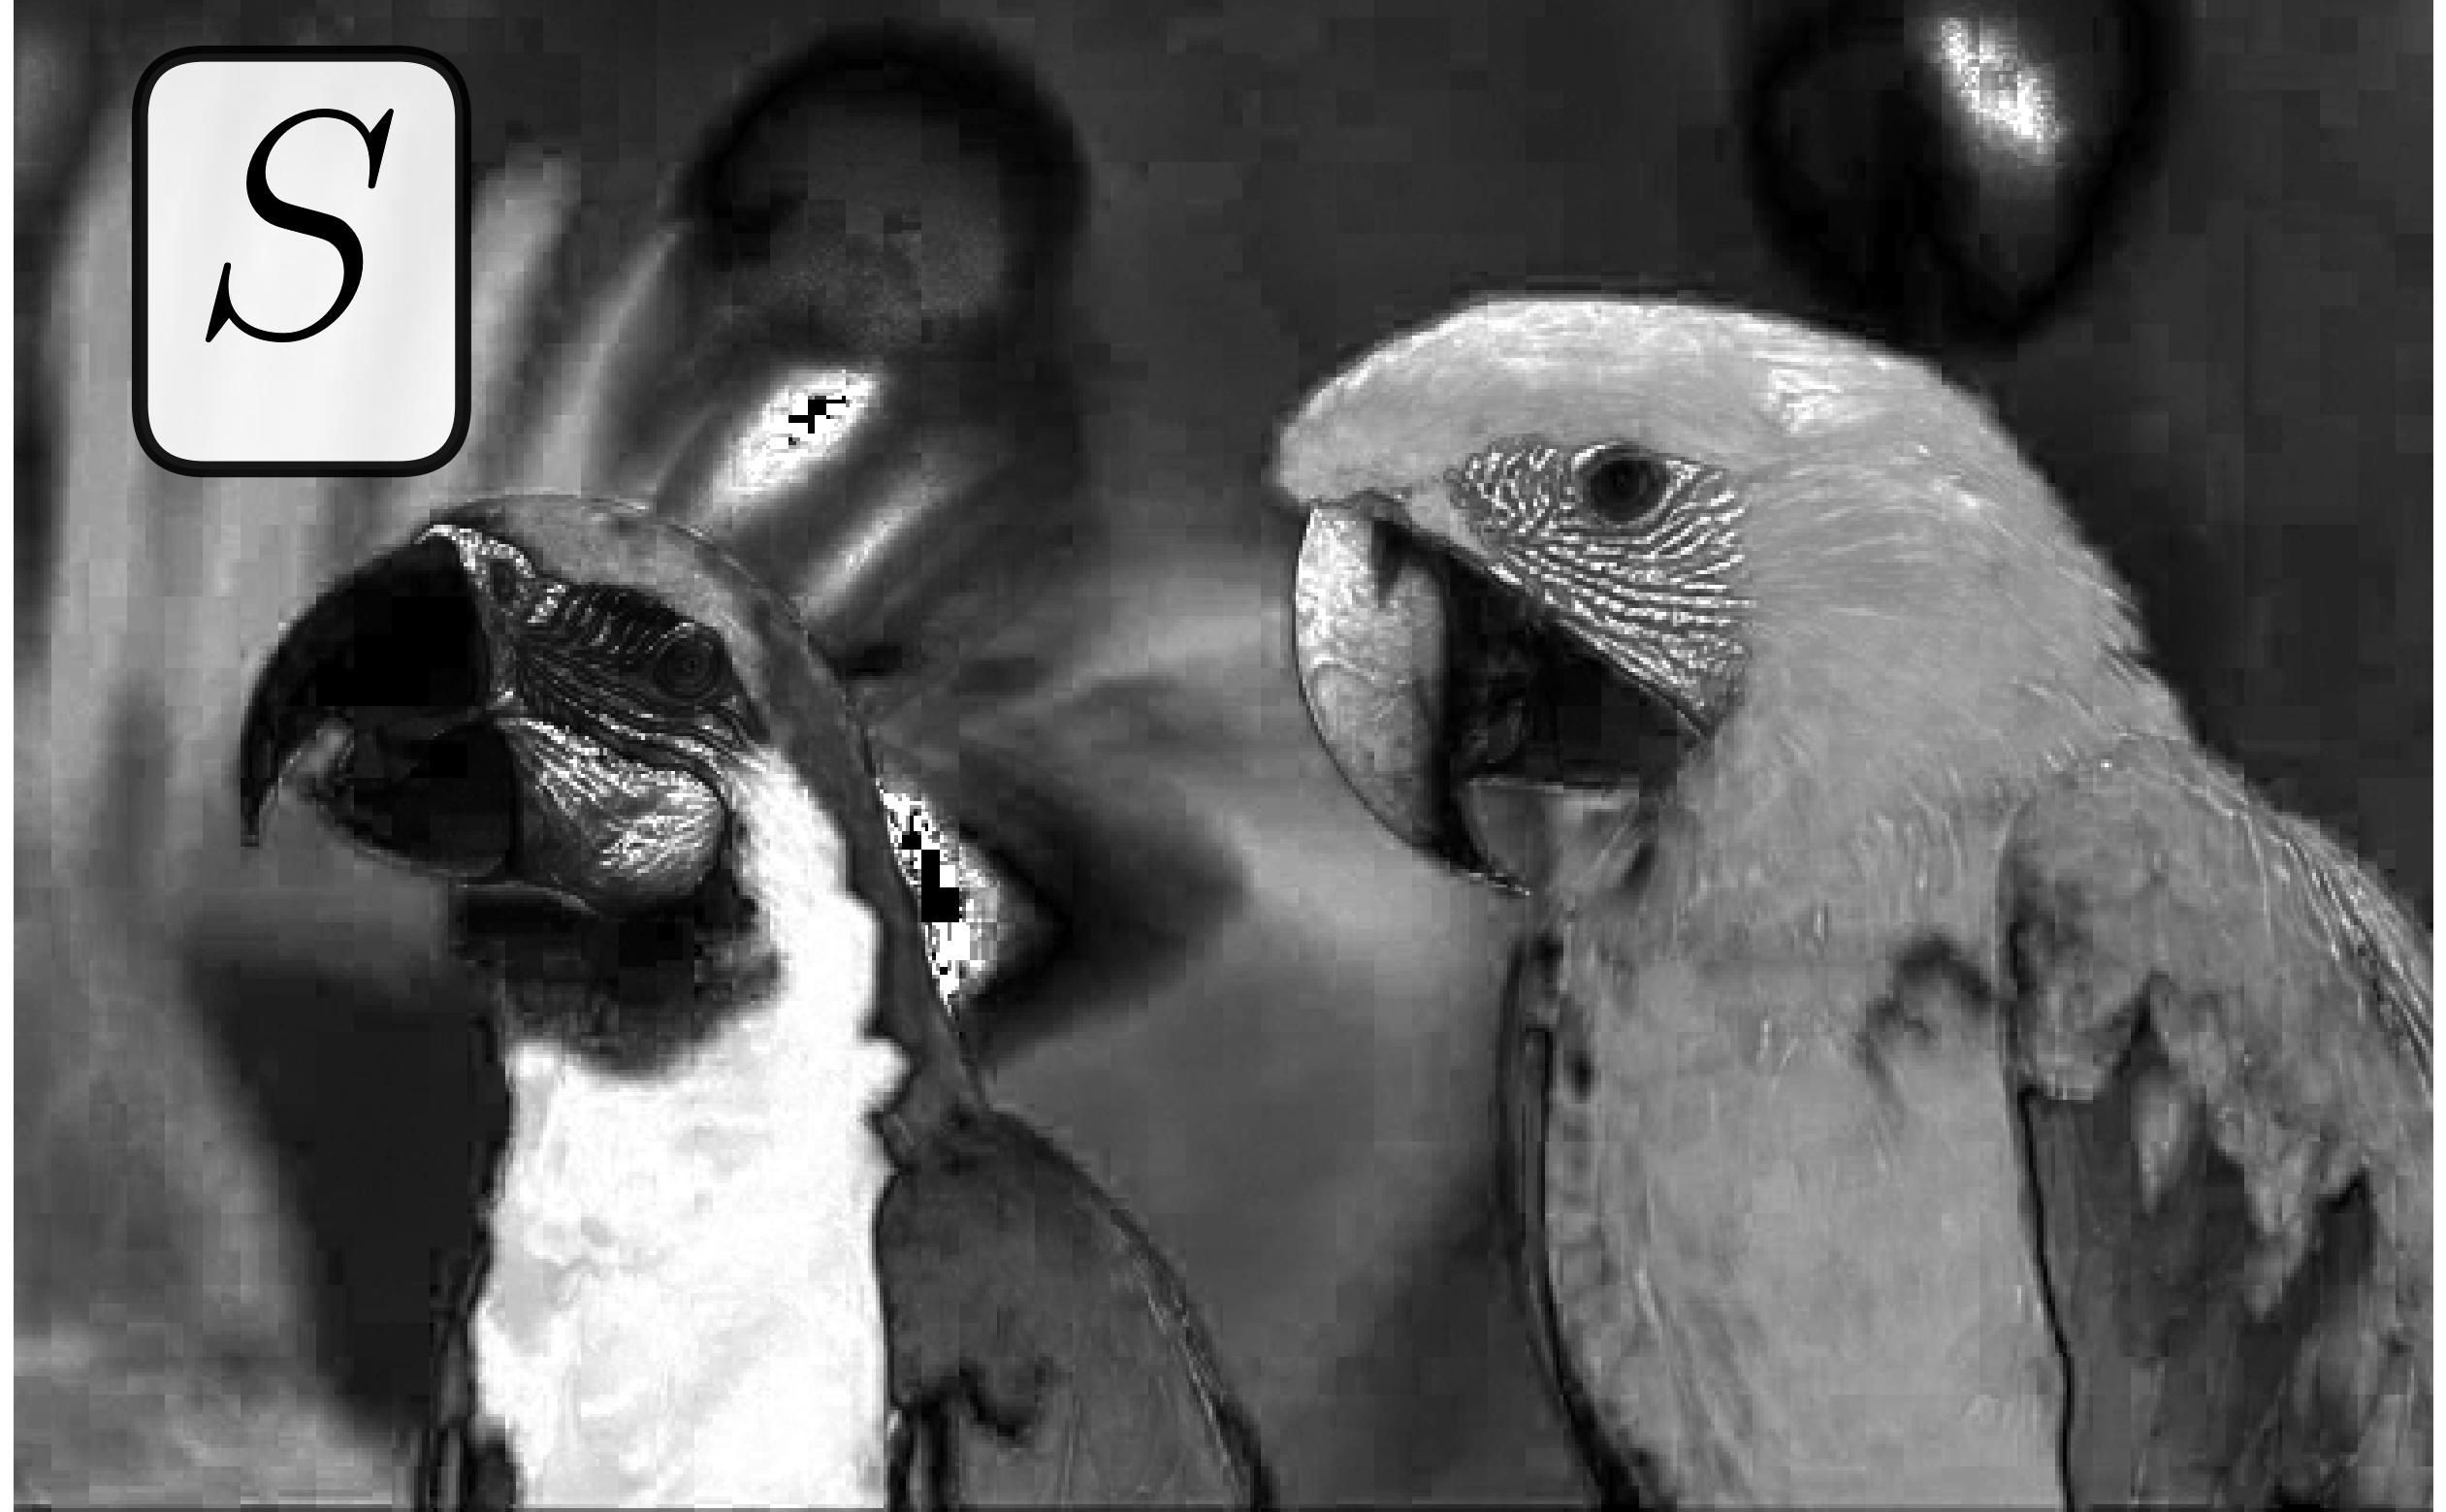
\includegraphics[width=\textwidth]{araras_S_HLS}
    \end{subfigure}
    ~ %add desired spacing between images, e. g. ~, \quad, \qquad, \hfill etc. 
      %(or a blank line to force the subfigure onto a new line)
    \begin{subfigure}[b]{0.3\textwidth}
        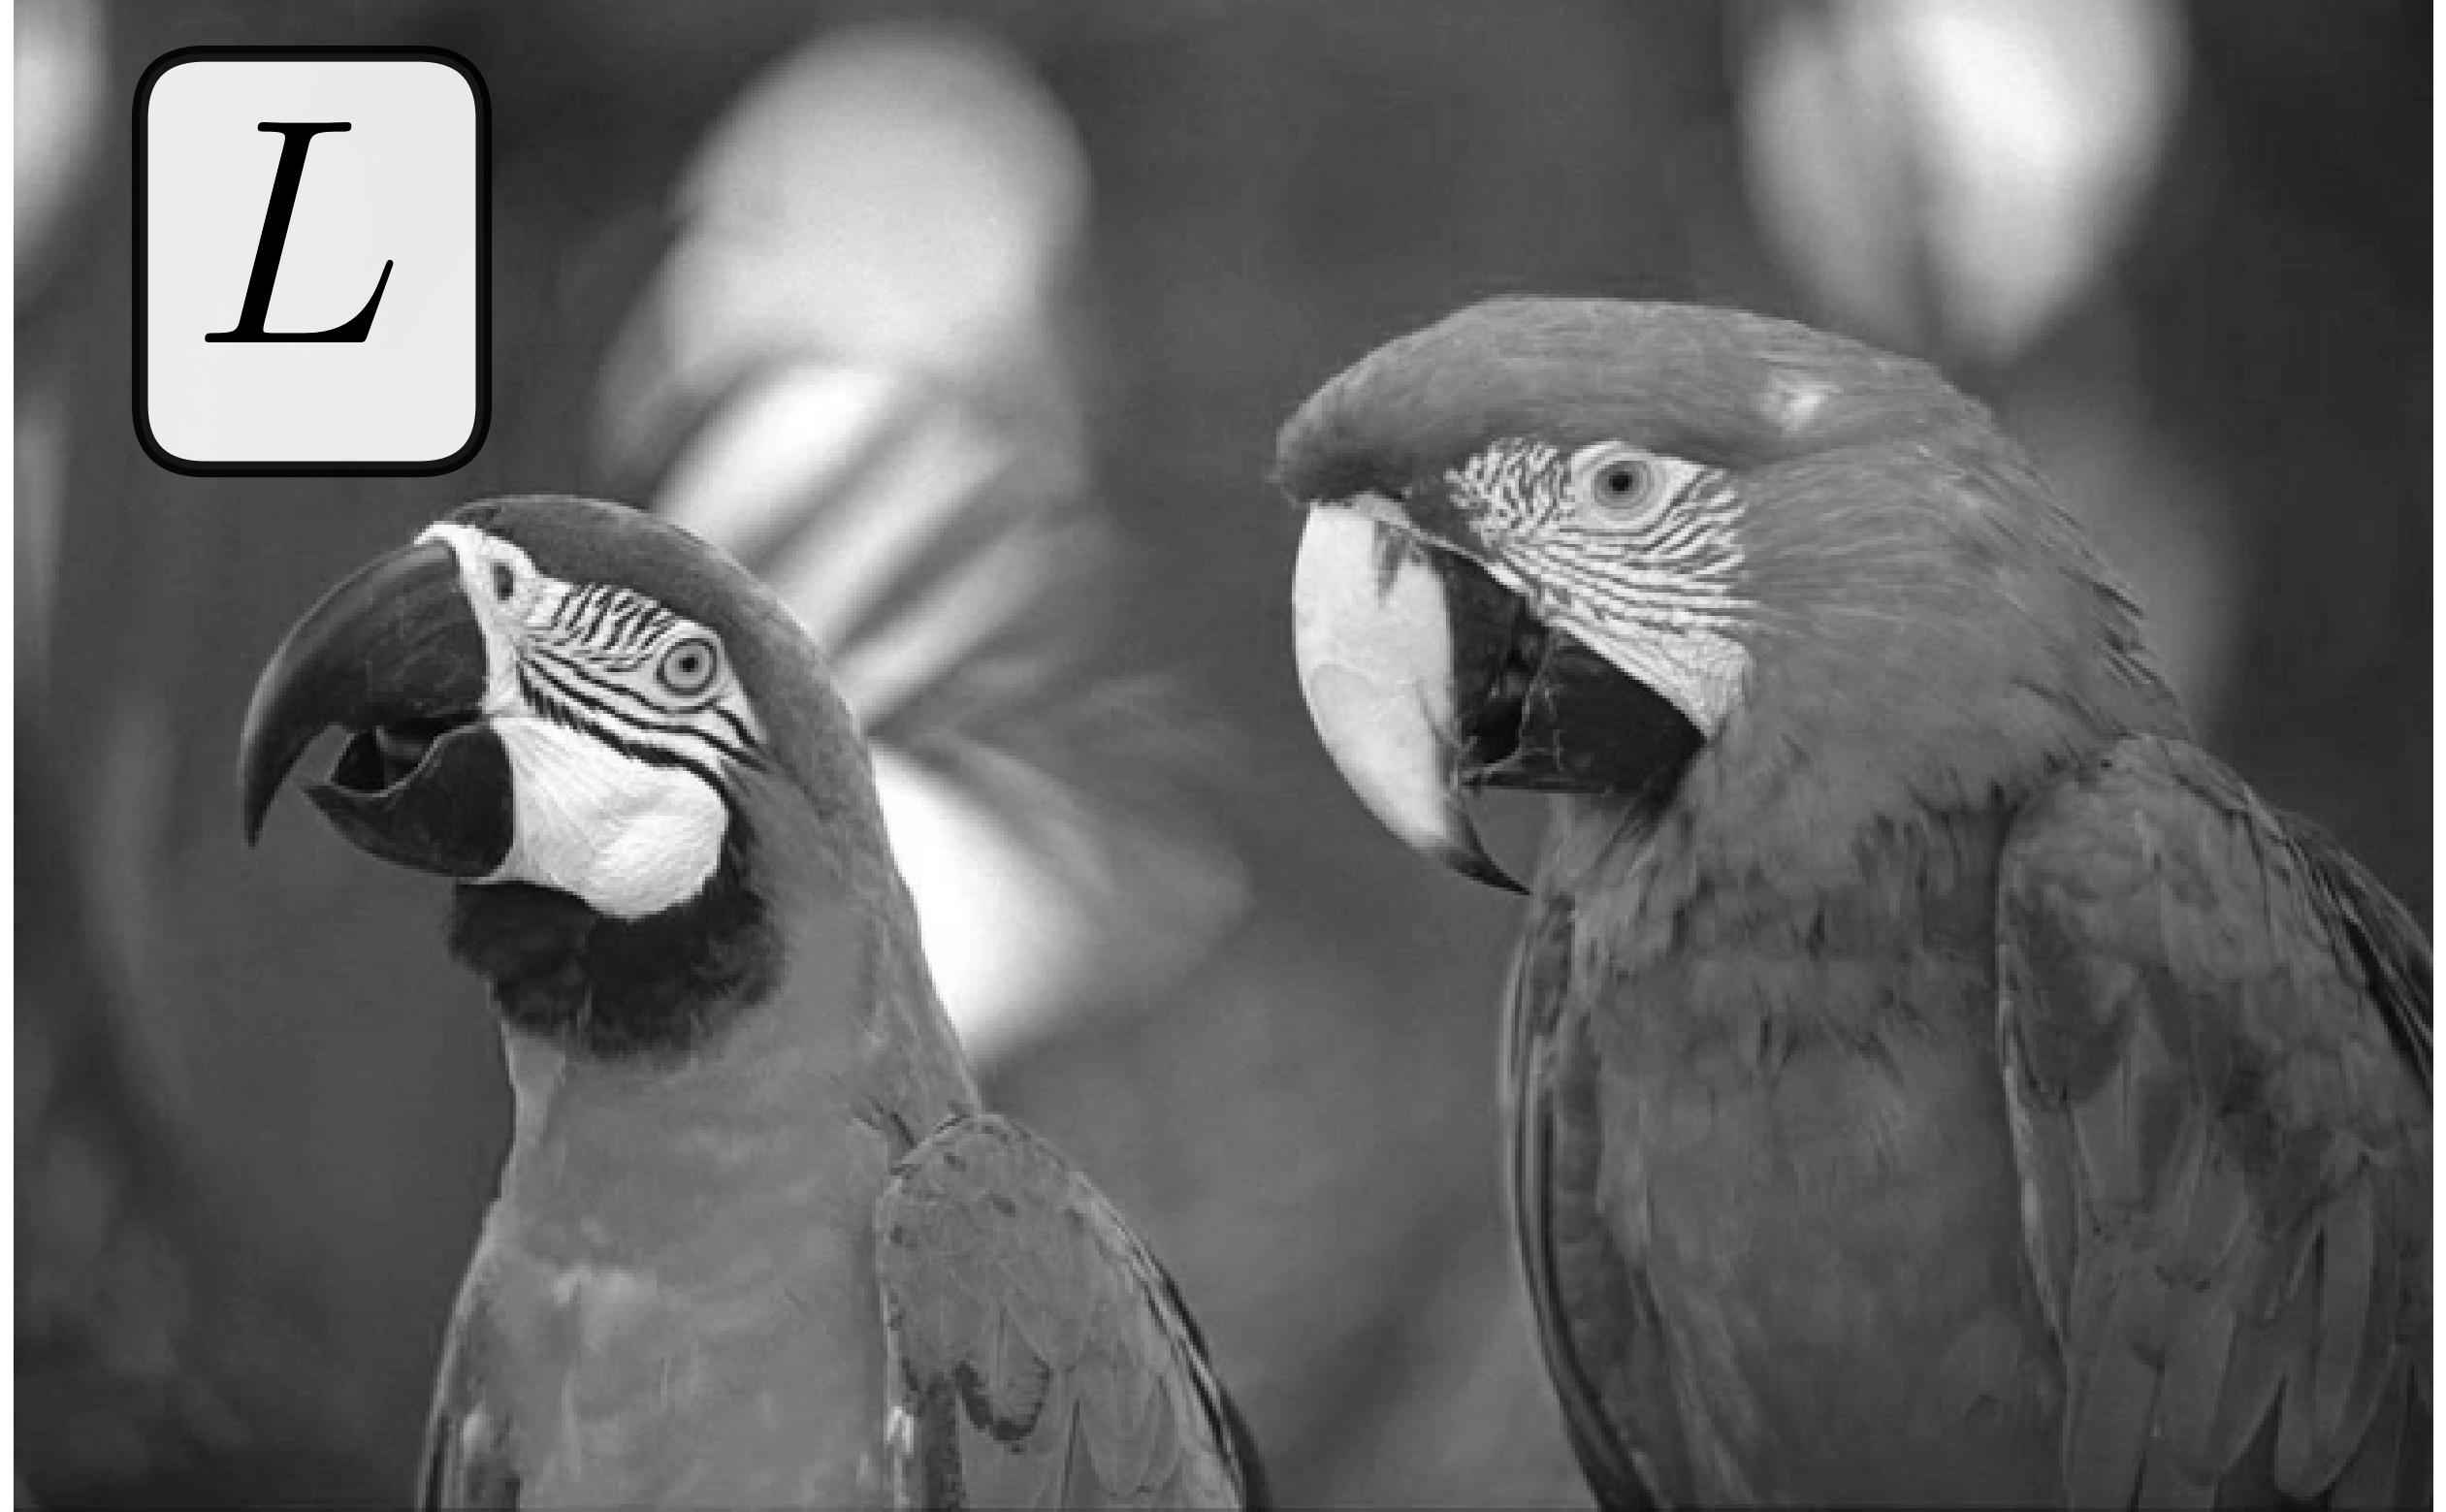
\includegraphics[width=\textwidth]{araras_L_HLS}
    \end{subfigure} \vspace{5pt} 
        
    \begin{subfigure}[t]{\dimexpr0.3\textwidth+20pt\relax}
    	\makebox[20pt]{\raisebox{35pt}{ \rotatebox[origin=c]{90} {\small \textsf{\textbf{LAB channels}}} }}%
    	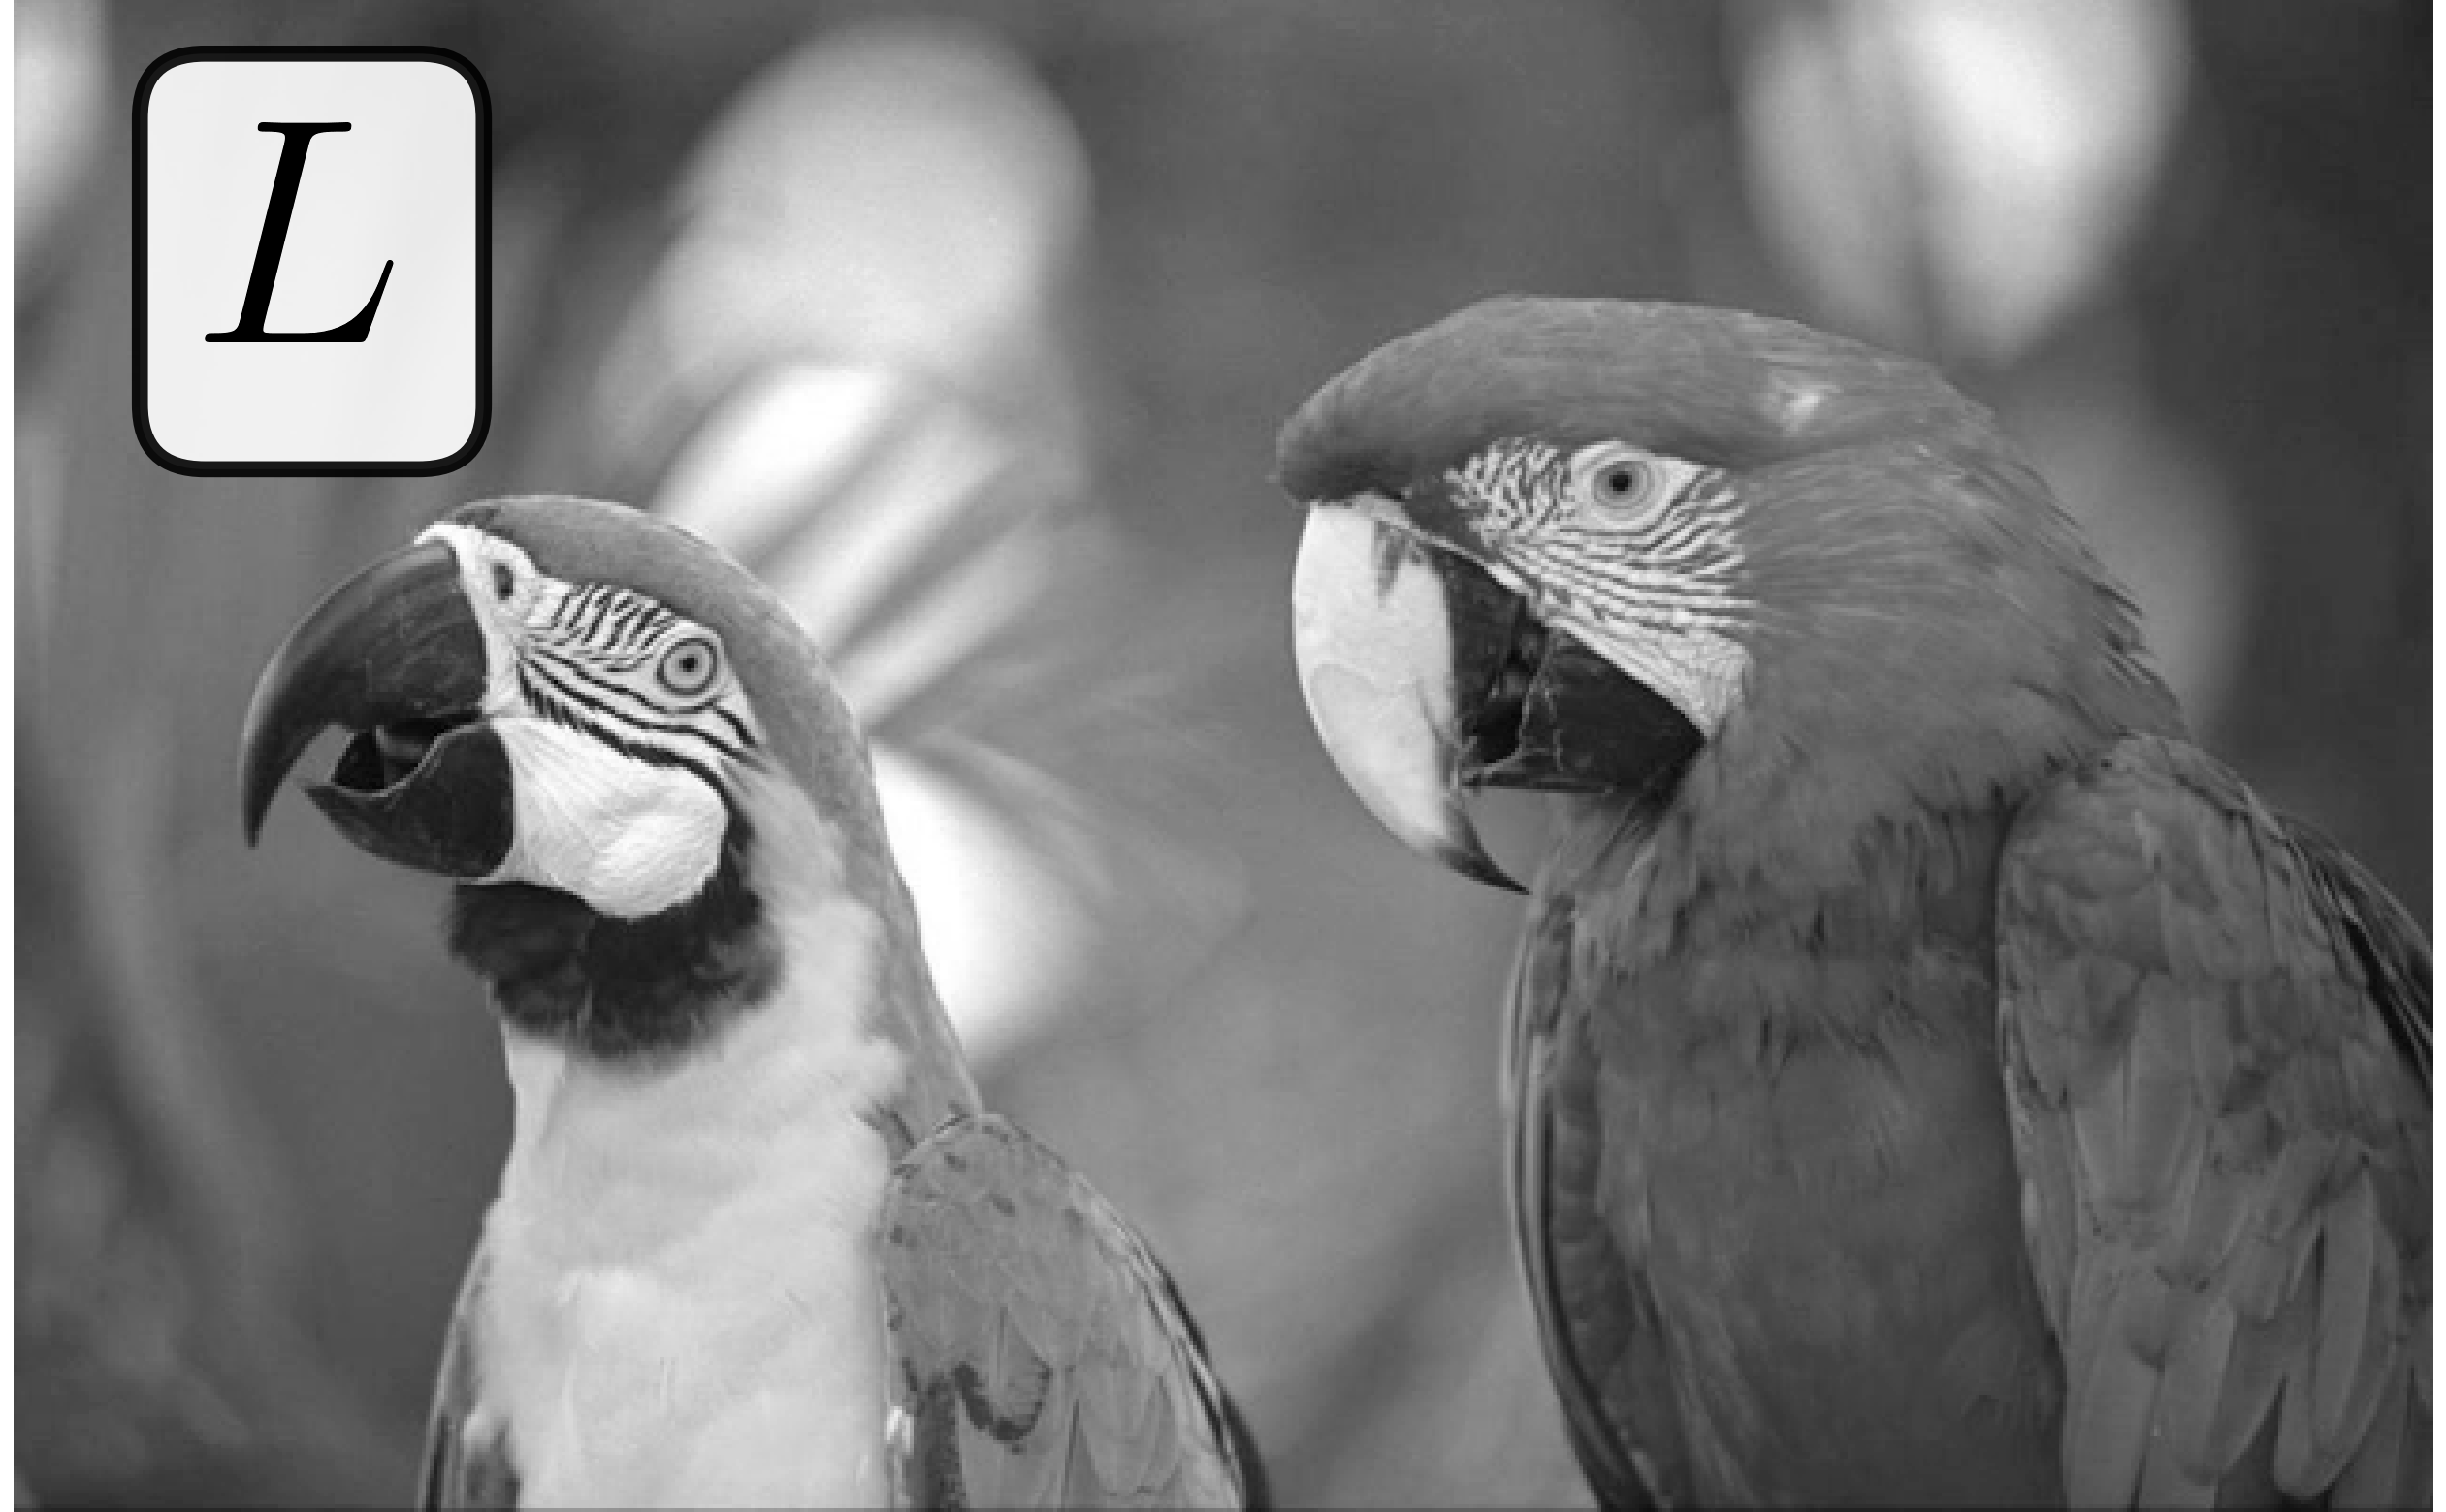
\includegraphics[width=\dimexpr\linewidth-20pt\relax]{araras_L_LAB}
    \end{subfigure}    
    ~ %add desired spacing between images, e. g. ~, \quad, \qquad, \hfill etc. 
      %(or a blank line to force the subfigure onto a new line)
    \begin{subfigure}[b]{0.3\textwidth}
        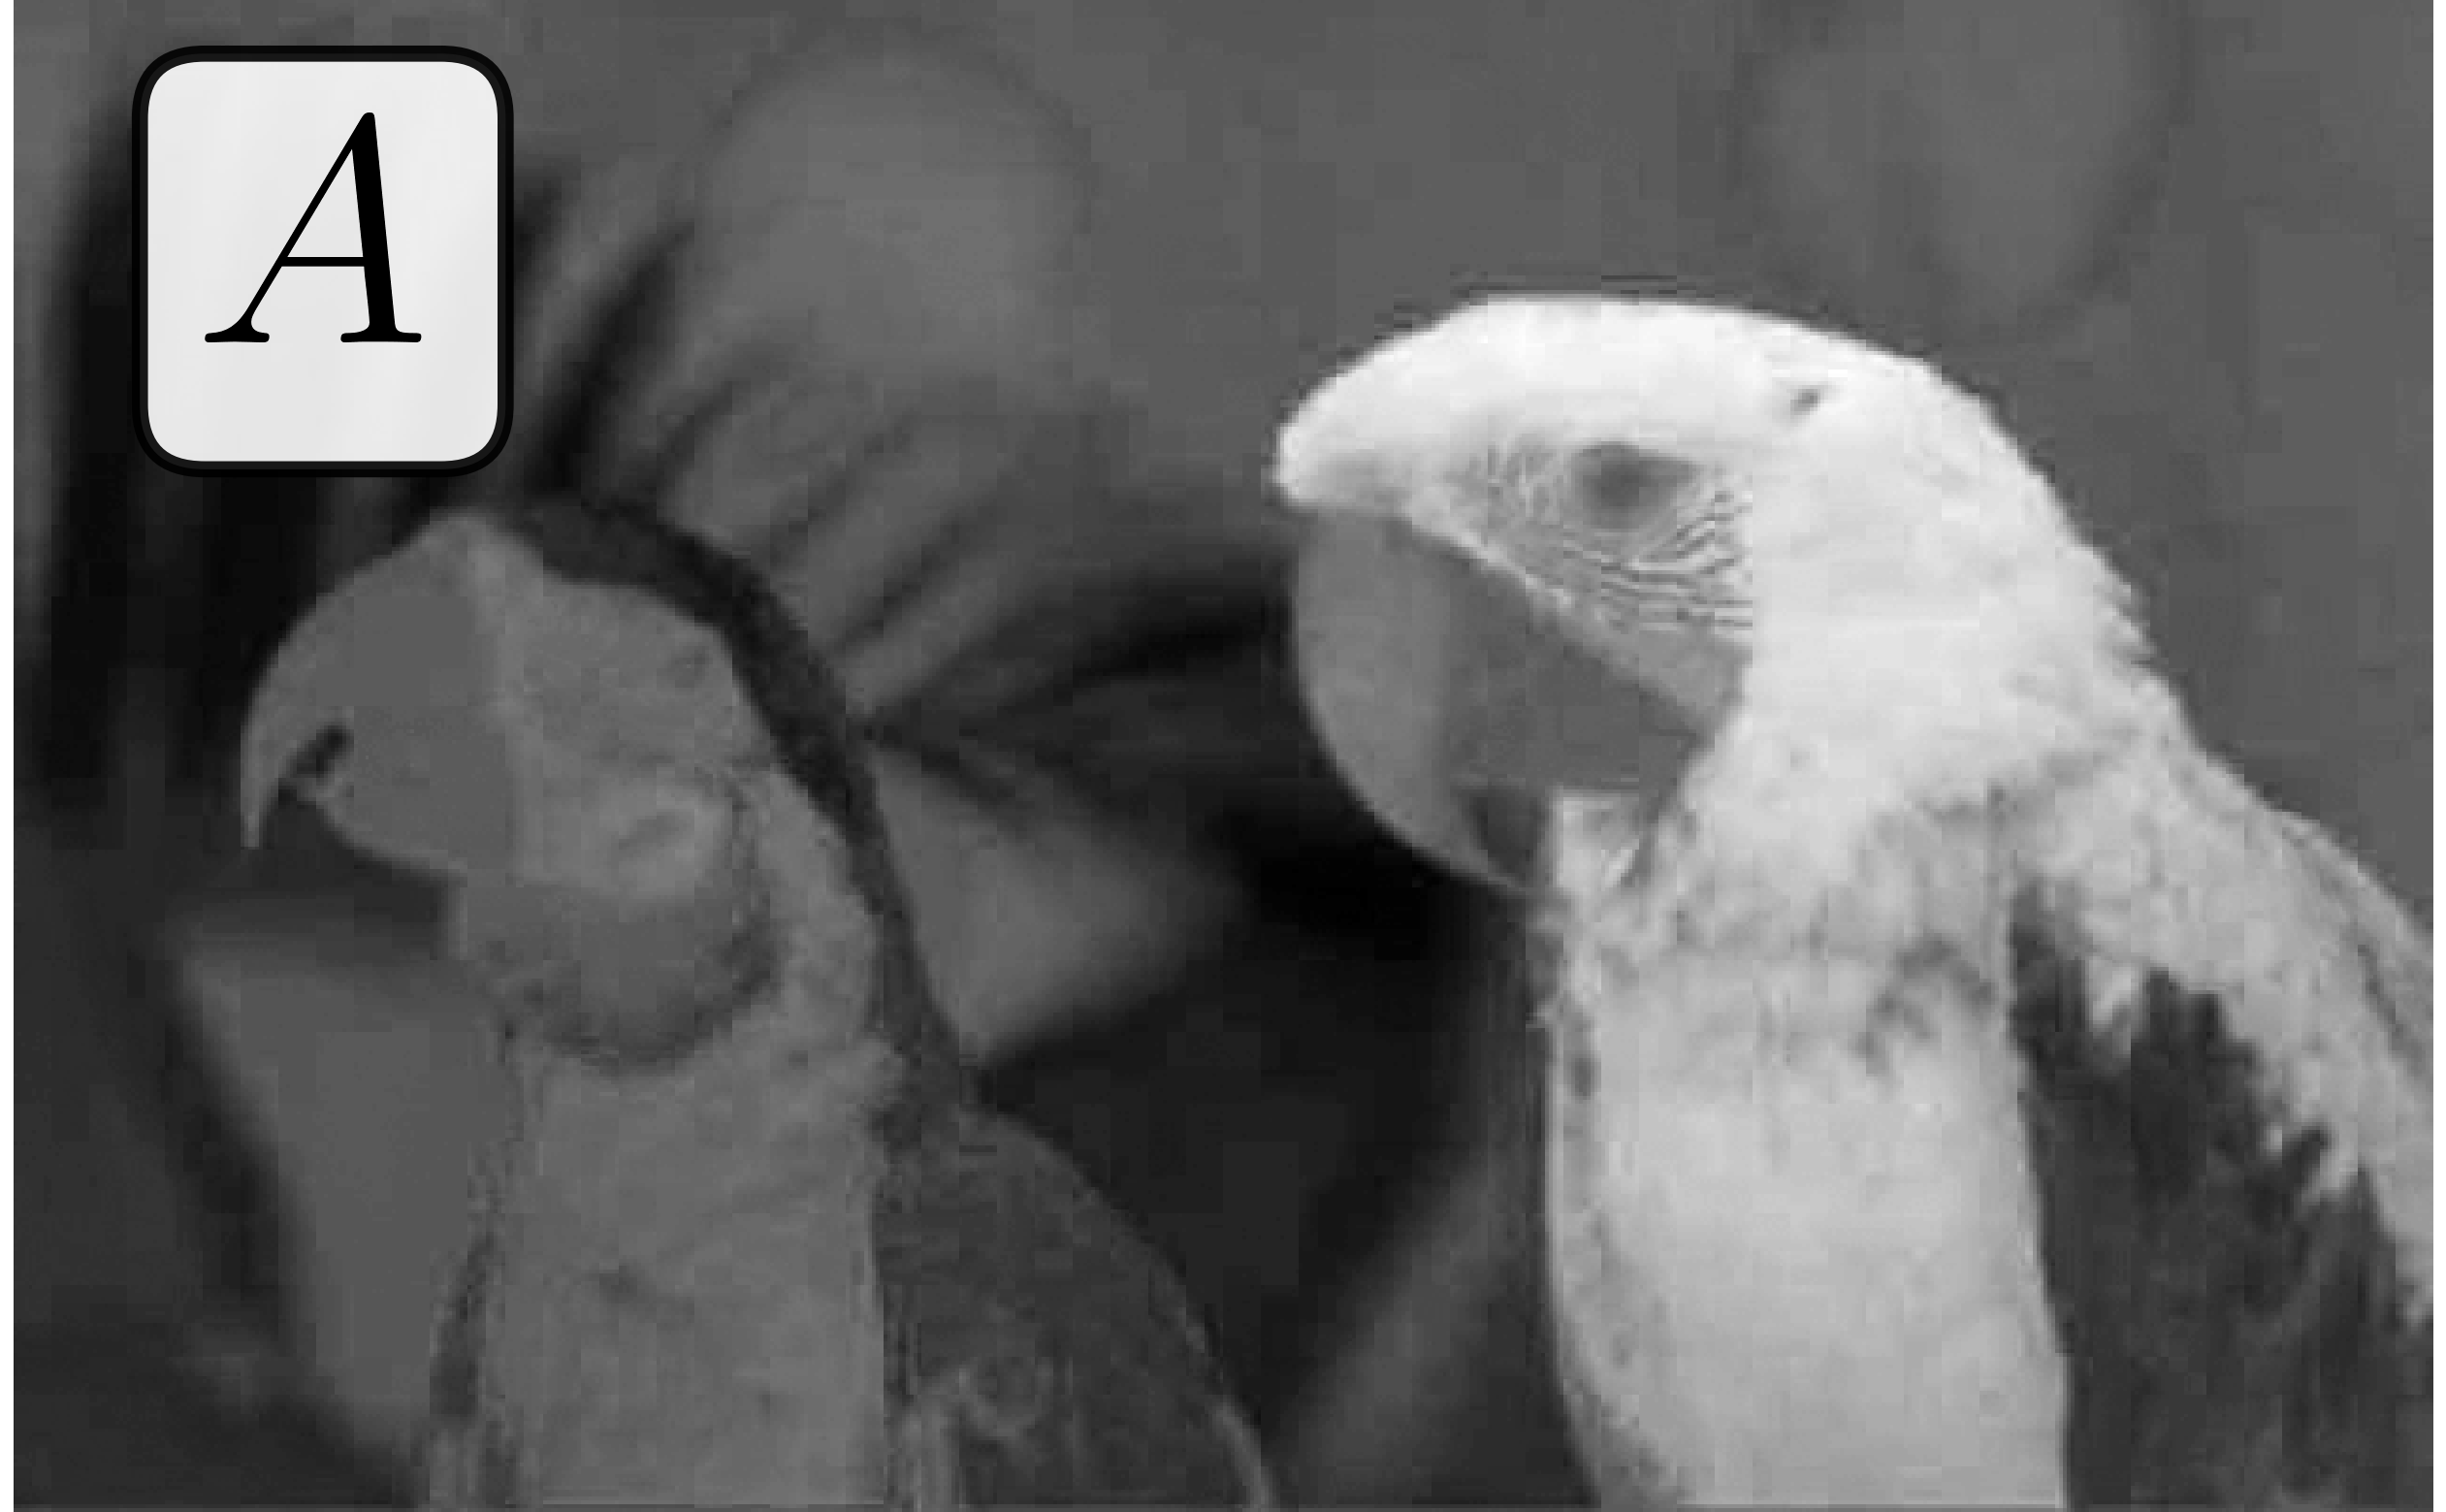
\includegraphics[width=\textwidth]{araras_A_LAB}
    \end{subfigure}
    ~ %add desired spacing between images, e. g. ~, \quad, \qquad, \hfill etc. 
      %(or a blank line to force the subfigure onto a new line)
    \begin{subfigure}[b]{0.3\textwidth}
        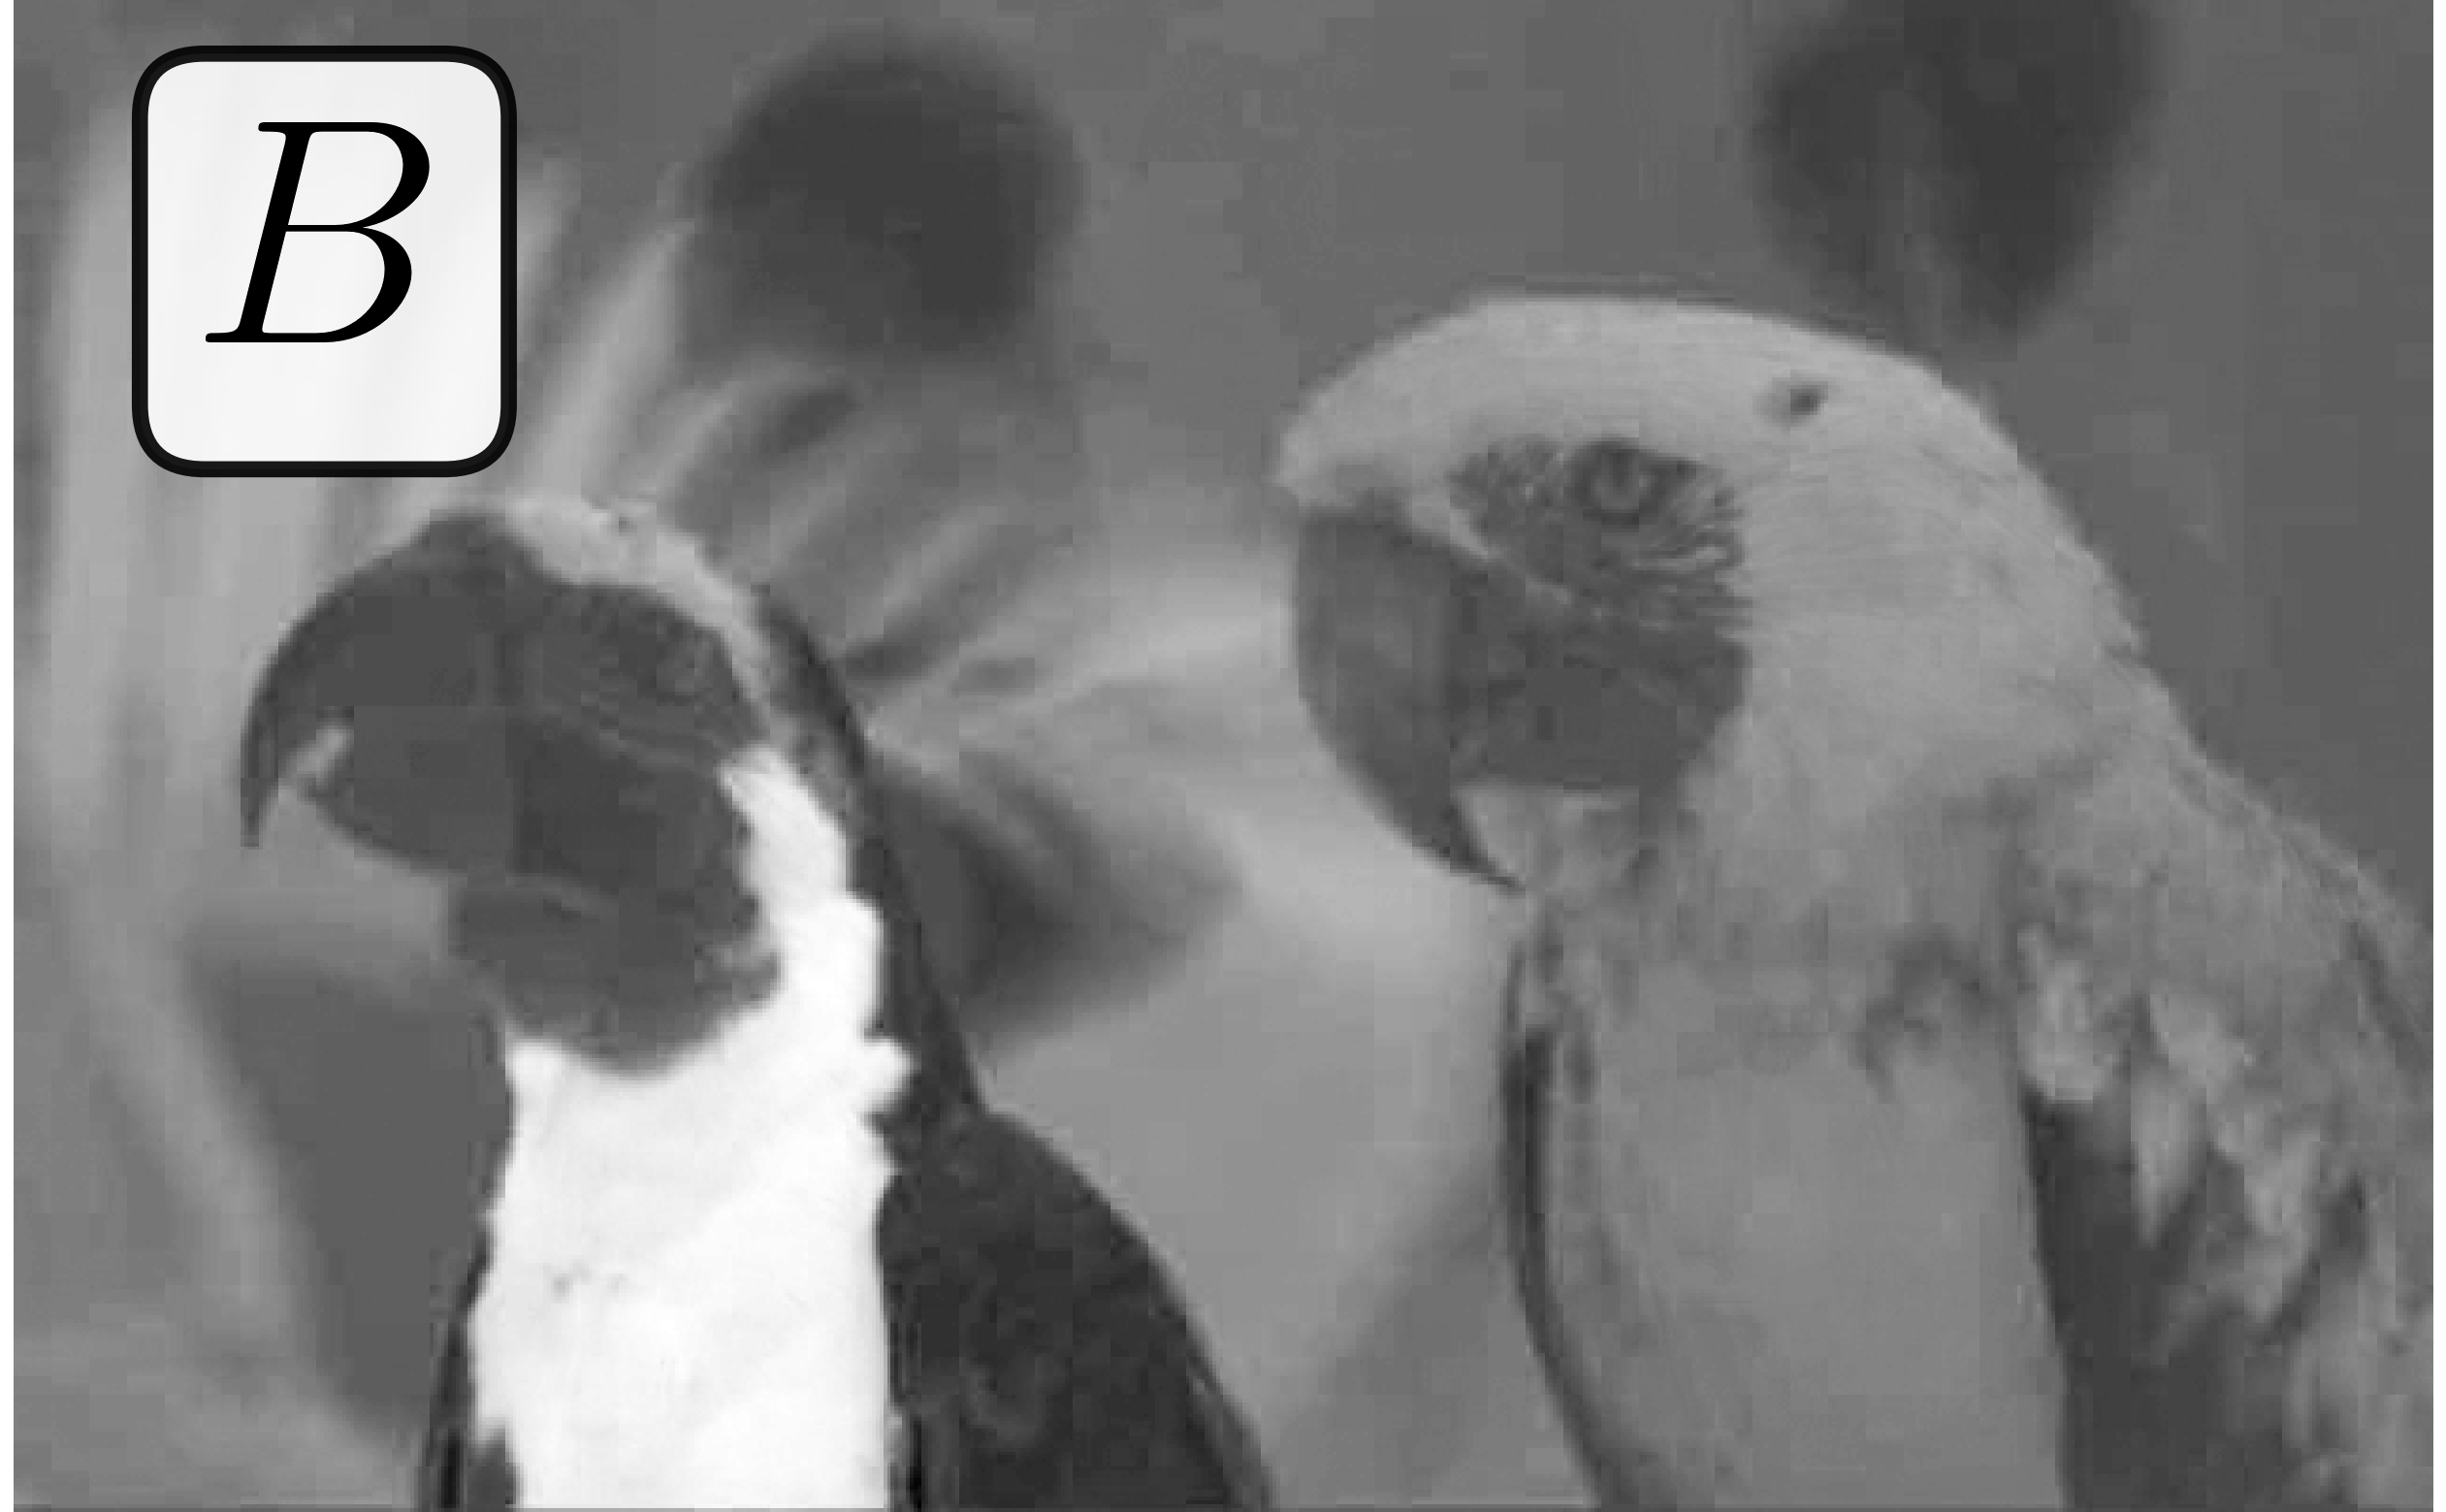
\includegraphics[width=\textwidth]{araras_B_LAB}
    \end{subfigure} 

	\caption{Color channels of an image in different color spaces in a grayscale}\label{fig:images_color_space}    
\end{figure}


The figure \ref{fig:images_color_space} shows the three channels of the different color spaces reviewed so far. The input image is a natural color image where the three main colors red, green, and blue naturally stand out. For the visualization of each color channels, we transform its channel values to the range $[0, 255]$ and 255 and displayed in a gray scale. 


\subsubsection{Luminance-chrominance color spaces}%Two-channel complex image representation

Color spaces mostly map the perception of color as a three-dimensional property. However, these dimensions can be encompassed in only two aspects, so we can classify them into luminance-chromaticity and luminance-chrominance color spaces. In both cases, luminance is the property that describes the brightness of light, however, both categories have different ways of defining color. Chromaticity-based spaces define color independently of luminance (or the luminance equivalent in a particular color space). In a chrominance-based space, the chrominance values of the image change as the light intensity varies.
  
We can obtain a color space based on chromaticity from the classic trichromatic models described in the previous section. The chromaticity of these models consists mainly of two independent parameters. For example, the $xyY$ color space, from which we obtaon the CIE chromaticity chart (see figure \ref{fig:chrom_diagram}), uses the X and Y dimensions to calculate chromaticity. In the case of RGB space, it is possible to obtain a space based on chromaticity following the same principle; using only the R and G channels for its calculation. For cylindrical color spaces (HSV, HSL), the independent parameters that describe chromaticity are the dimensions of hue and colorfulness (saturation).

\begin{figure}[!ht] 
	\centering
	\begin{subfigure}[b]{0.48\textwidth}
		\centering
		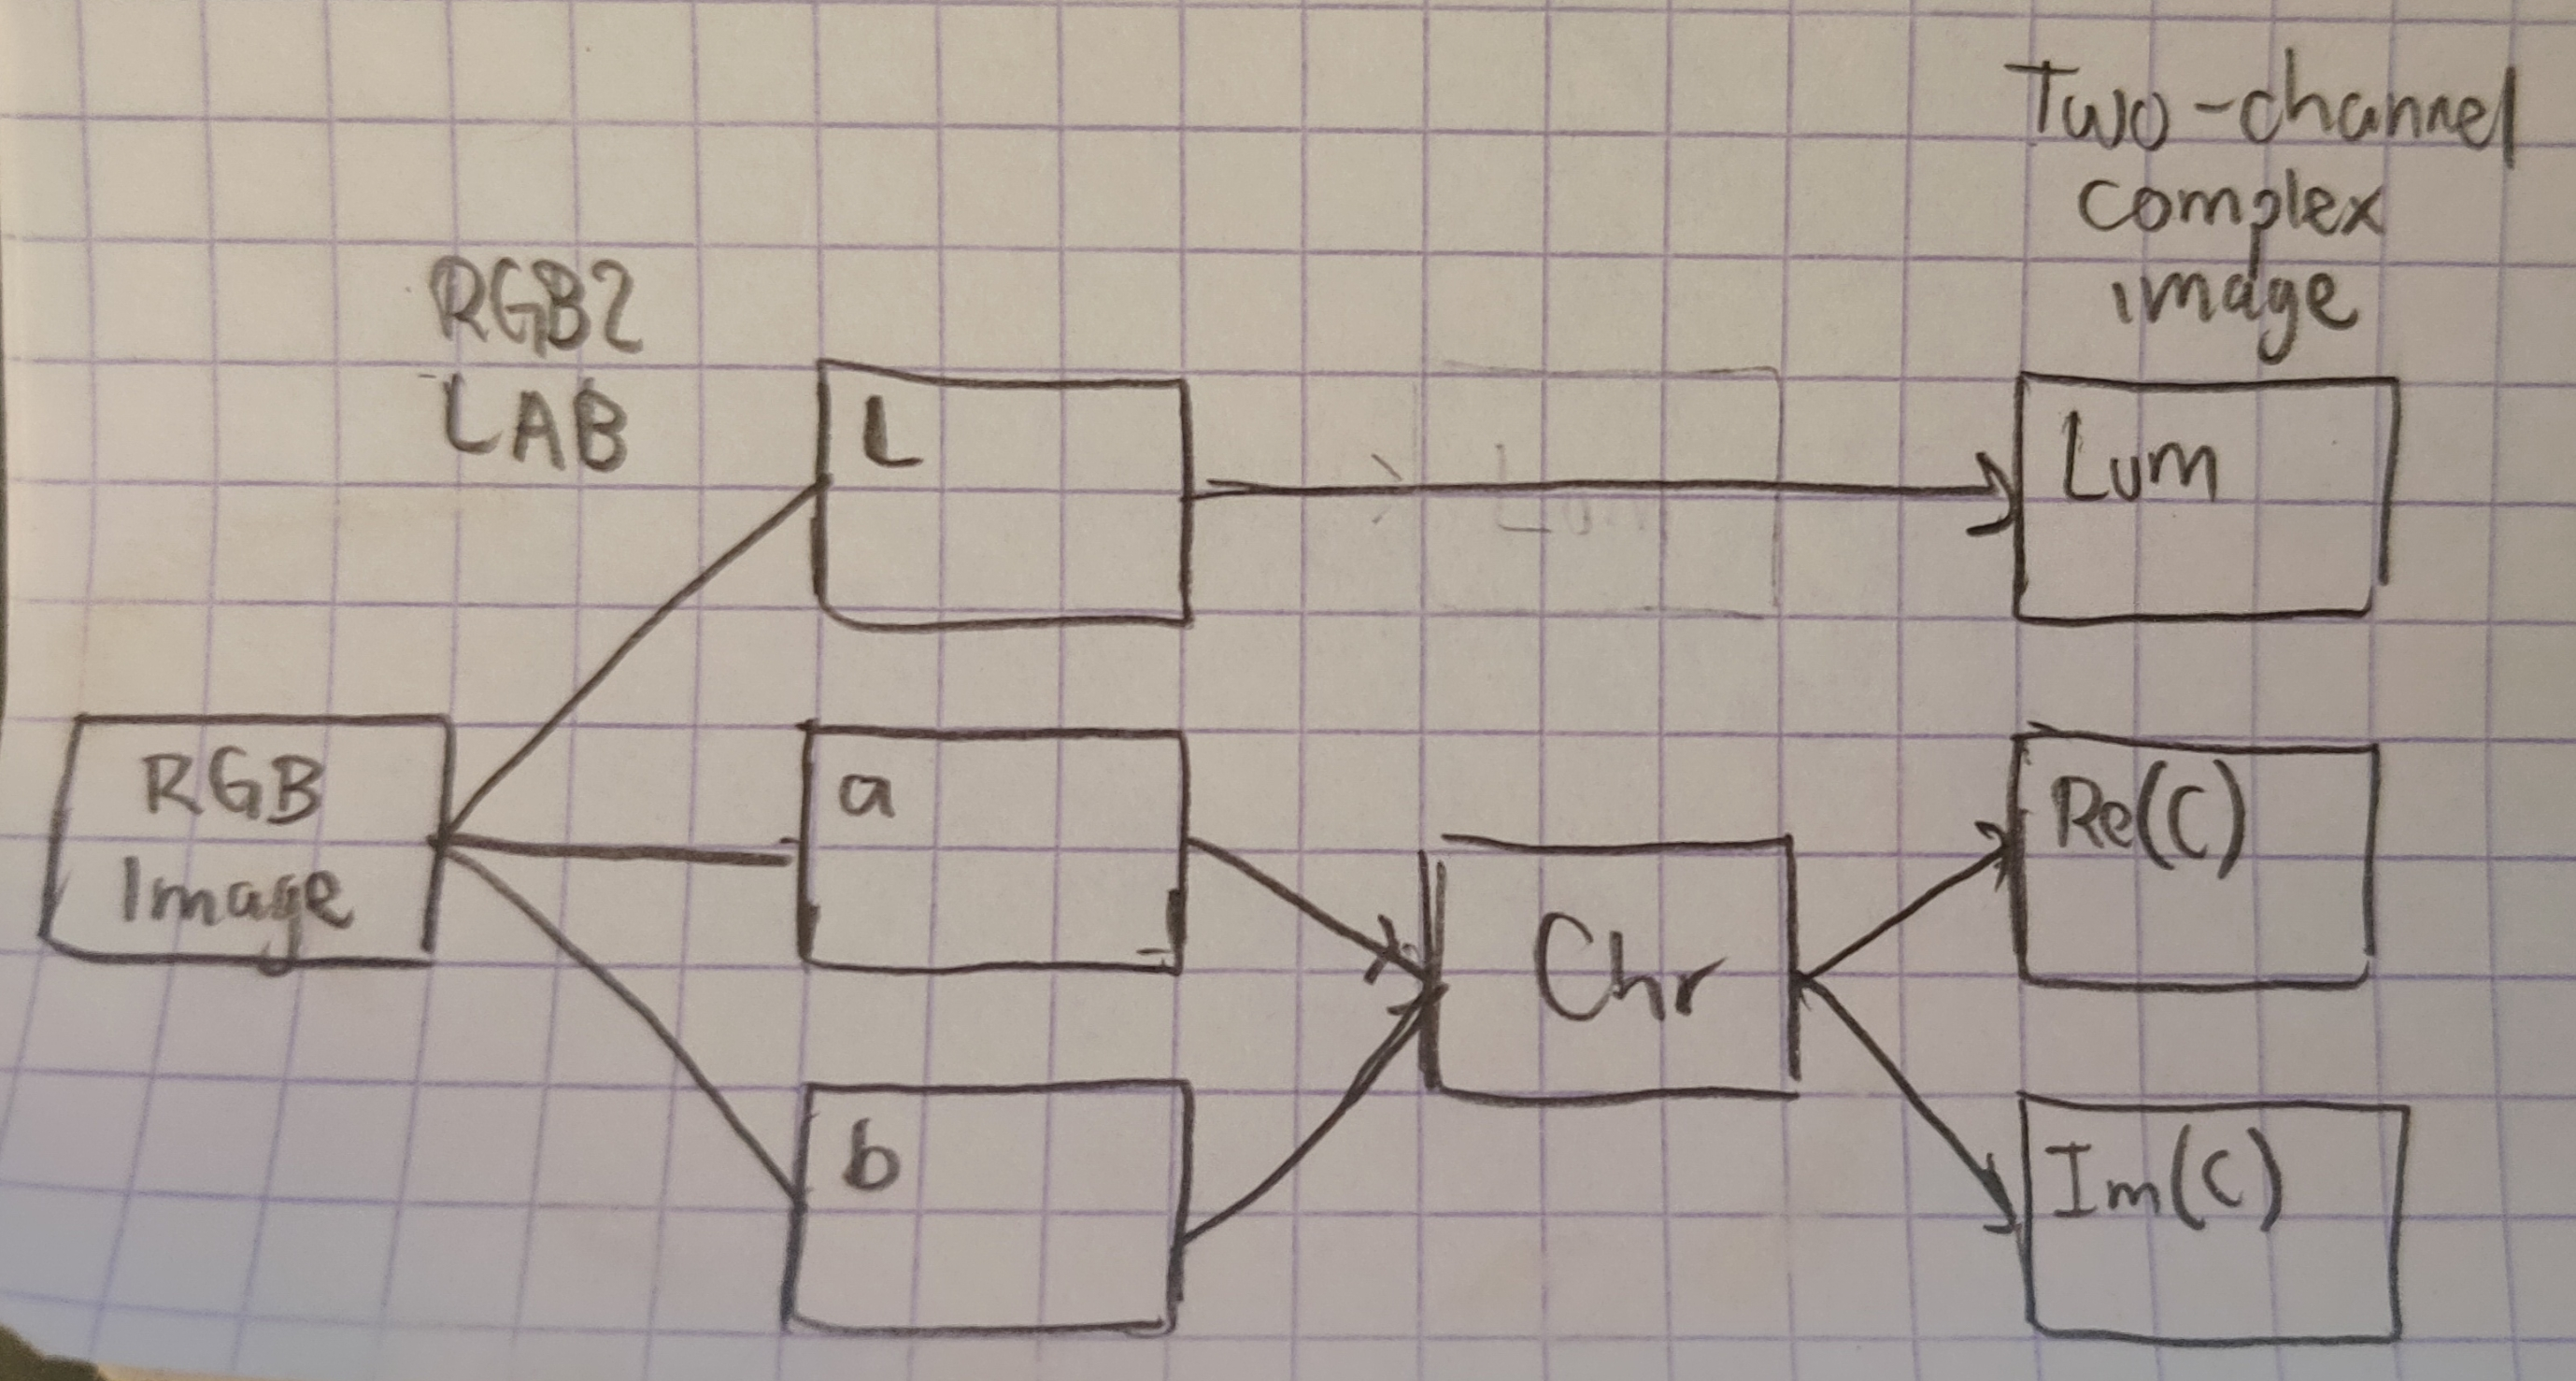
\includegraphics[width=\textwidth]{lab_complex_color}
		\caption{}	
		\label{fig:lab_complex_color}
	\end{subfigure}
	~%add desired spacing between images, e. g. ~, \quad, \qquad, \hfill etc. 
	%(or a blank line to force the subfigure onto a new line)
	\begin{subfigure}[b]{0.48\textwidth}
		\centering
		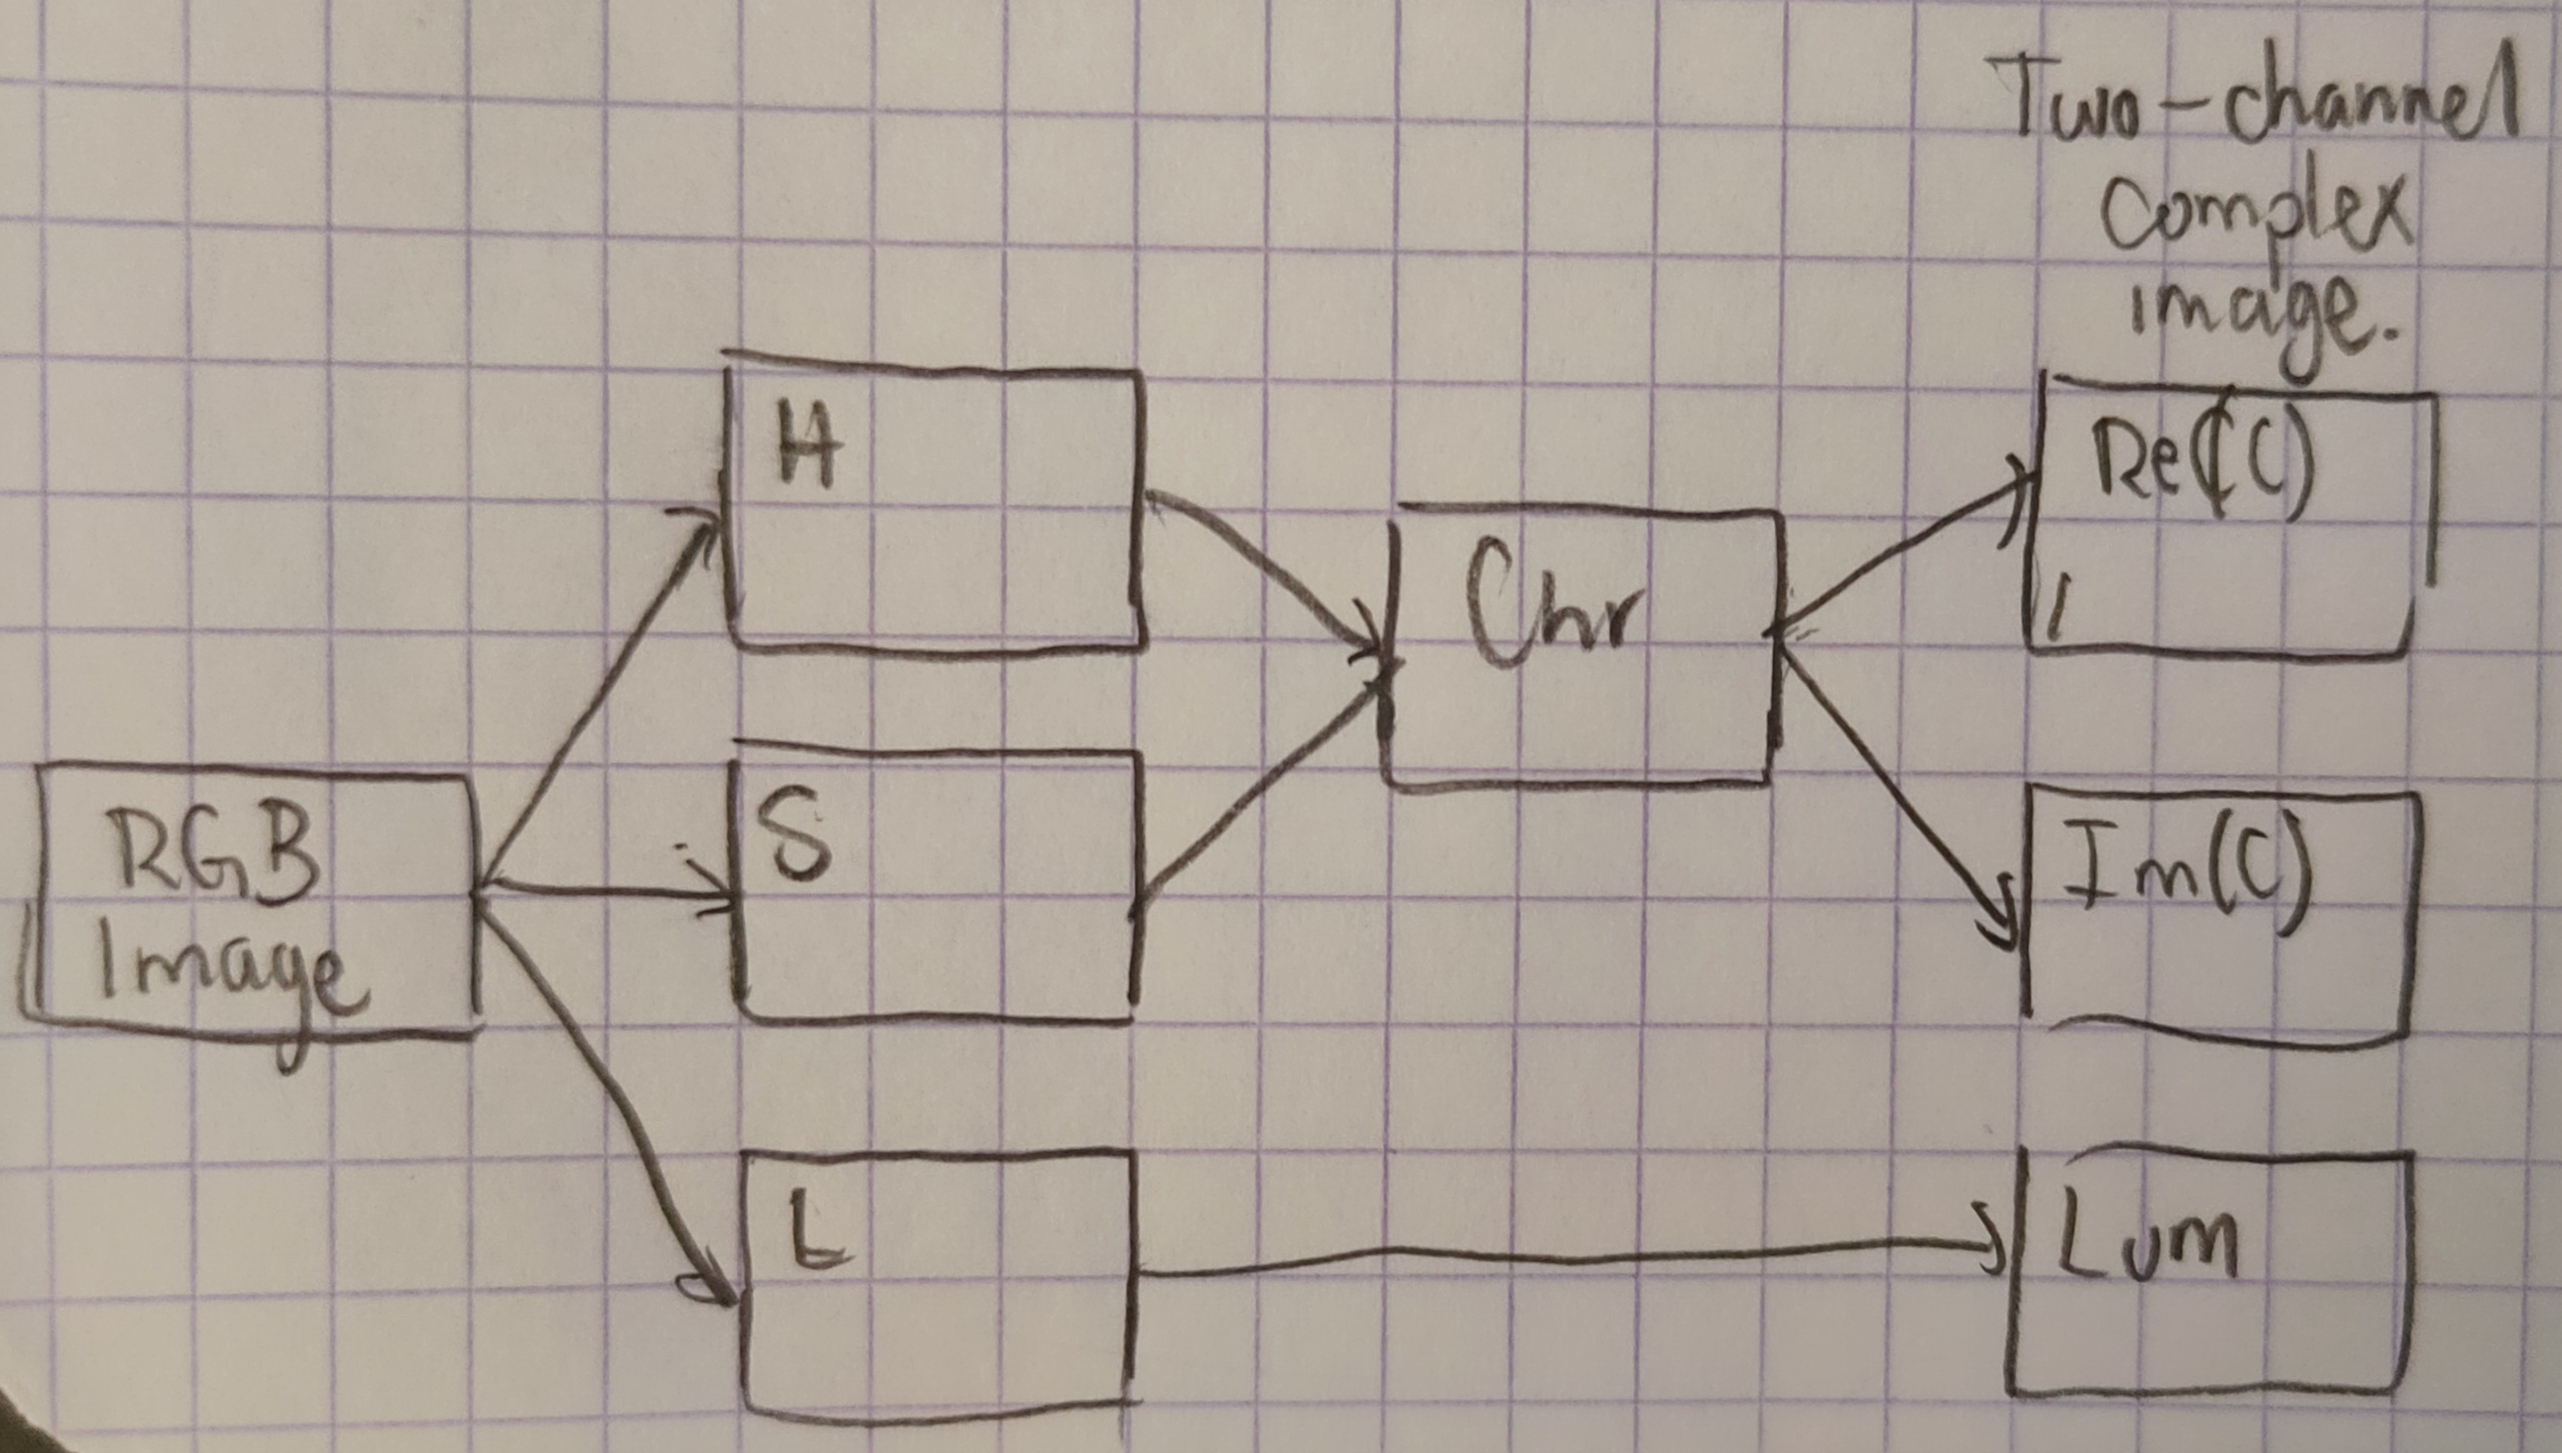
\includegraphics[width=\textwidth]{hsl_complex_color}
		\caption{}	
		\label{fig:hsl_complex_color}
	\end{subfigure}
	~%add desired spacing between images, e. g. ~, \quad, \qquad, \hfill etc. 
	%(or a blank line to force the subfigure onto a new line)
	\begin{subfigure}[b]{0.48\textwidth}
		\centering
		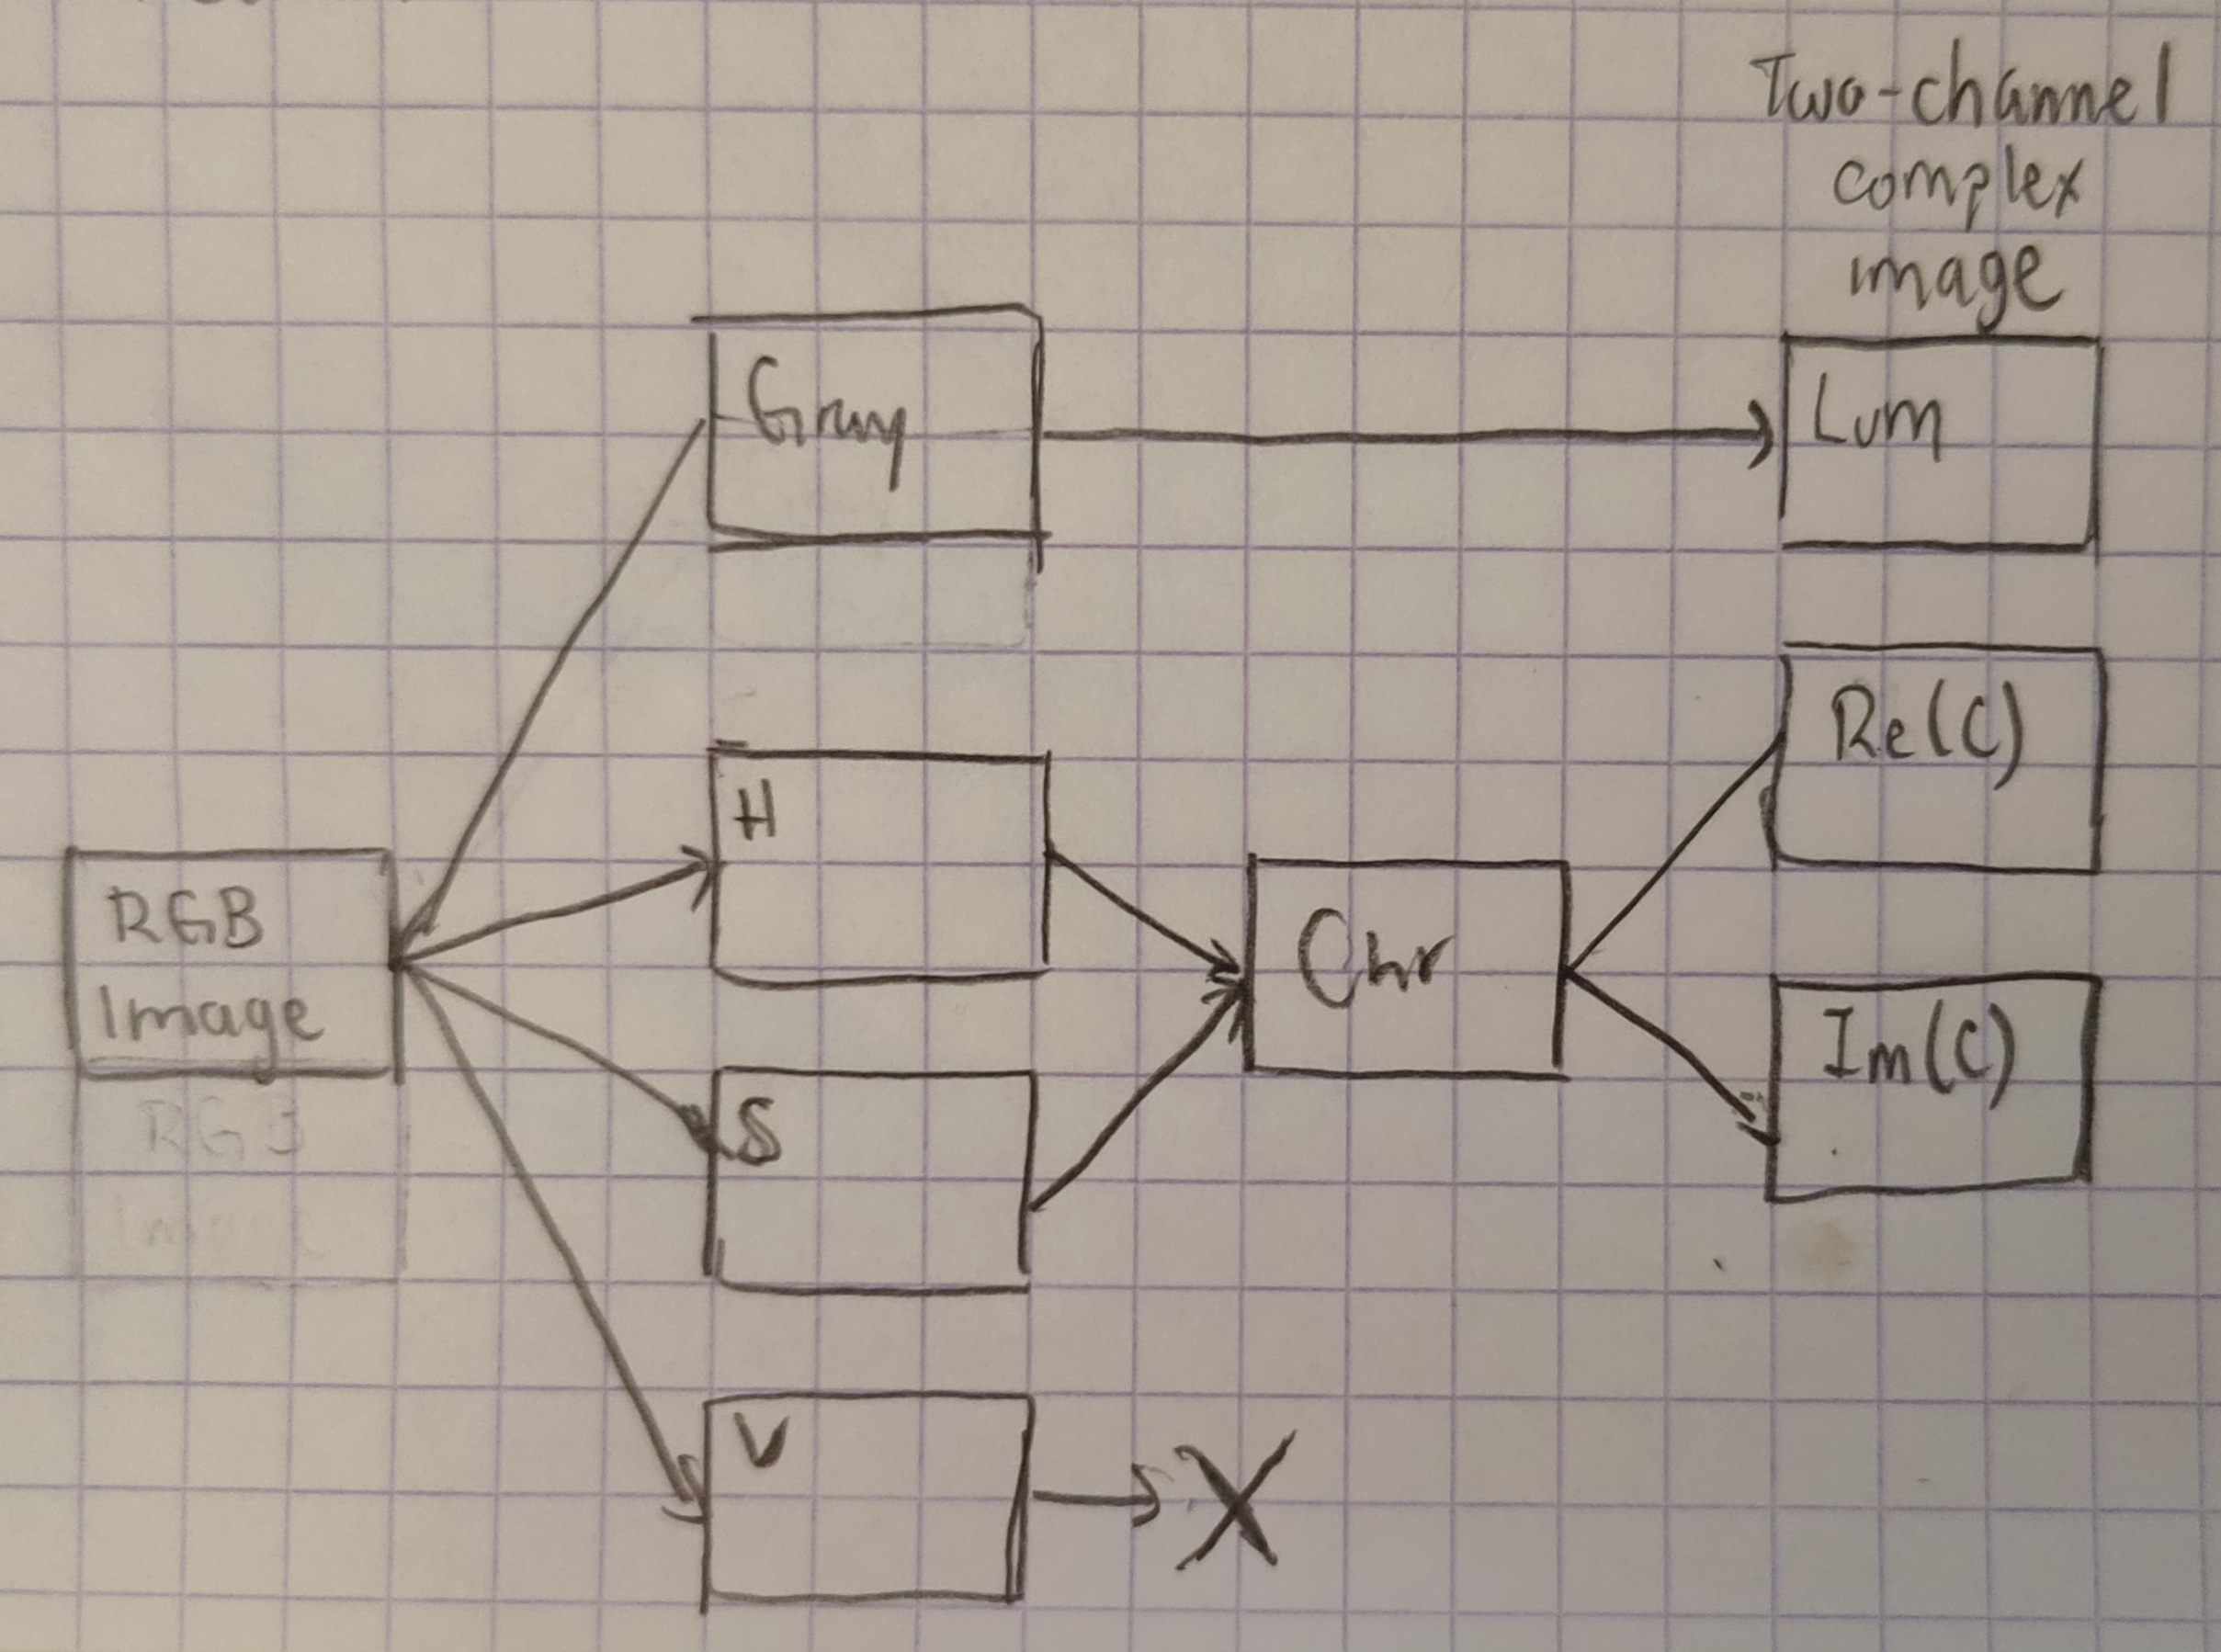
\includegraphics[width=\textwidth]{hsv_complex_color}
		\caption{ }	
		\label{fig:hsv_complex_color}
	\end{subfigure}
	
	\caption{}
	\label{fig:complex_color_spaces}
\end{figure}

Chromaticity-based models are reputed for their use in image editing and color correction. However, chrominance-based spaces are useful if we are looking for a uniform distribution of the color information in an image. Some examples of color spaces in this category are CIELAB and CIELUV. In them, the colorfulness information of an image is found in channels A and B (resp. U and V) and the final color is defined by the brightness of the light defined by the luminance L.

The use of spaces based on luminance-chrominance reduces the dimensionality of the color to two channels $L$ and $C$. To make this two-channel color representation possible, we combine the values of channels A and B with the chrominance function.
\begin{equation}\label{eq:chrominance_lab}
    C(x,y) = a^*(x,y) + ib^*(x,y)
\end{equation}

In the same way, it is possible to obtain a luminance-chrominance color space using the dimensions of the cylindrical HSV/HSL color spaces. The chrominance is described by the hue H and saturation S channels such that the complex chrominance channel is defined by the function
\begin{equation}\label{eq:chrominance_hsv}
    C = S e^{iH}
\end{equation}

These representations have the advantage of reducing the dimensionality of the color information. In image processing, these color spaces can be obtained from the transformation of the image from the RGB space to the LAB, HSV and HSL spaces, from which the chrominance variables and consequently the complex chrominance channel are obtained. Regarding luminance, it may differ depending on the input color space. For example, for the LAB and HSL spaces, this variable is naturally defined, however, in the case of the HSV space, the luminance channel is obtained from the transformation of the RGB input image to a grayscale image. The figure \ref{fig:complex_color_spaces} shows the diagrams for obtaining an image represented in two channels.


\begin{figure}[!ht]
    \begin{subfigure}[t]{\dimexpr0.3\textwidth+20pt\relax}
    	\makebox[20pt]{\raisebox{35pt}{ \rotatebox[origin=c]{90} {\small \textsf{\textbf{Input image}}} }}%
    	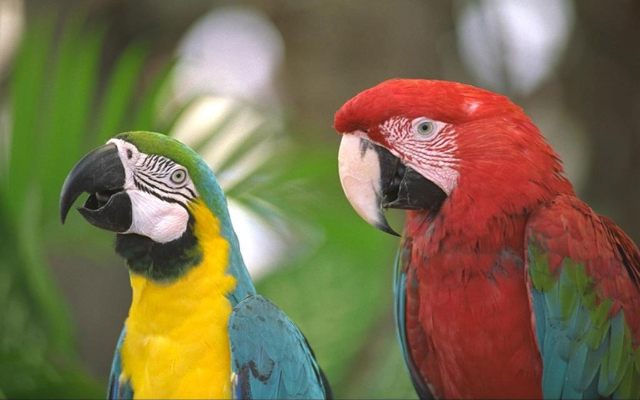
\includegraphics[width=\dimexpr\linewidth-20pt\relax]{araras}
    \end{subfigure} \\    
     
    \begin{subfigure}[t]{\dimexpr0.3\textwidth+20pt\relax}
    	\makebox[20pt]{\raisebox{35pt}{ \rotatebox[origin=c]{90} {\small \textsf{\textbf{HSV luma/chroma}}} }}%
    	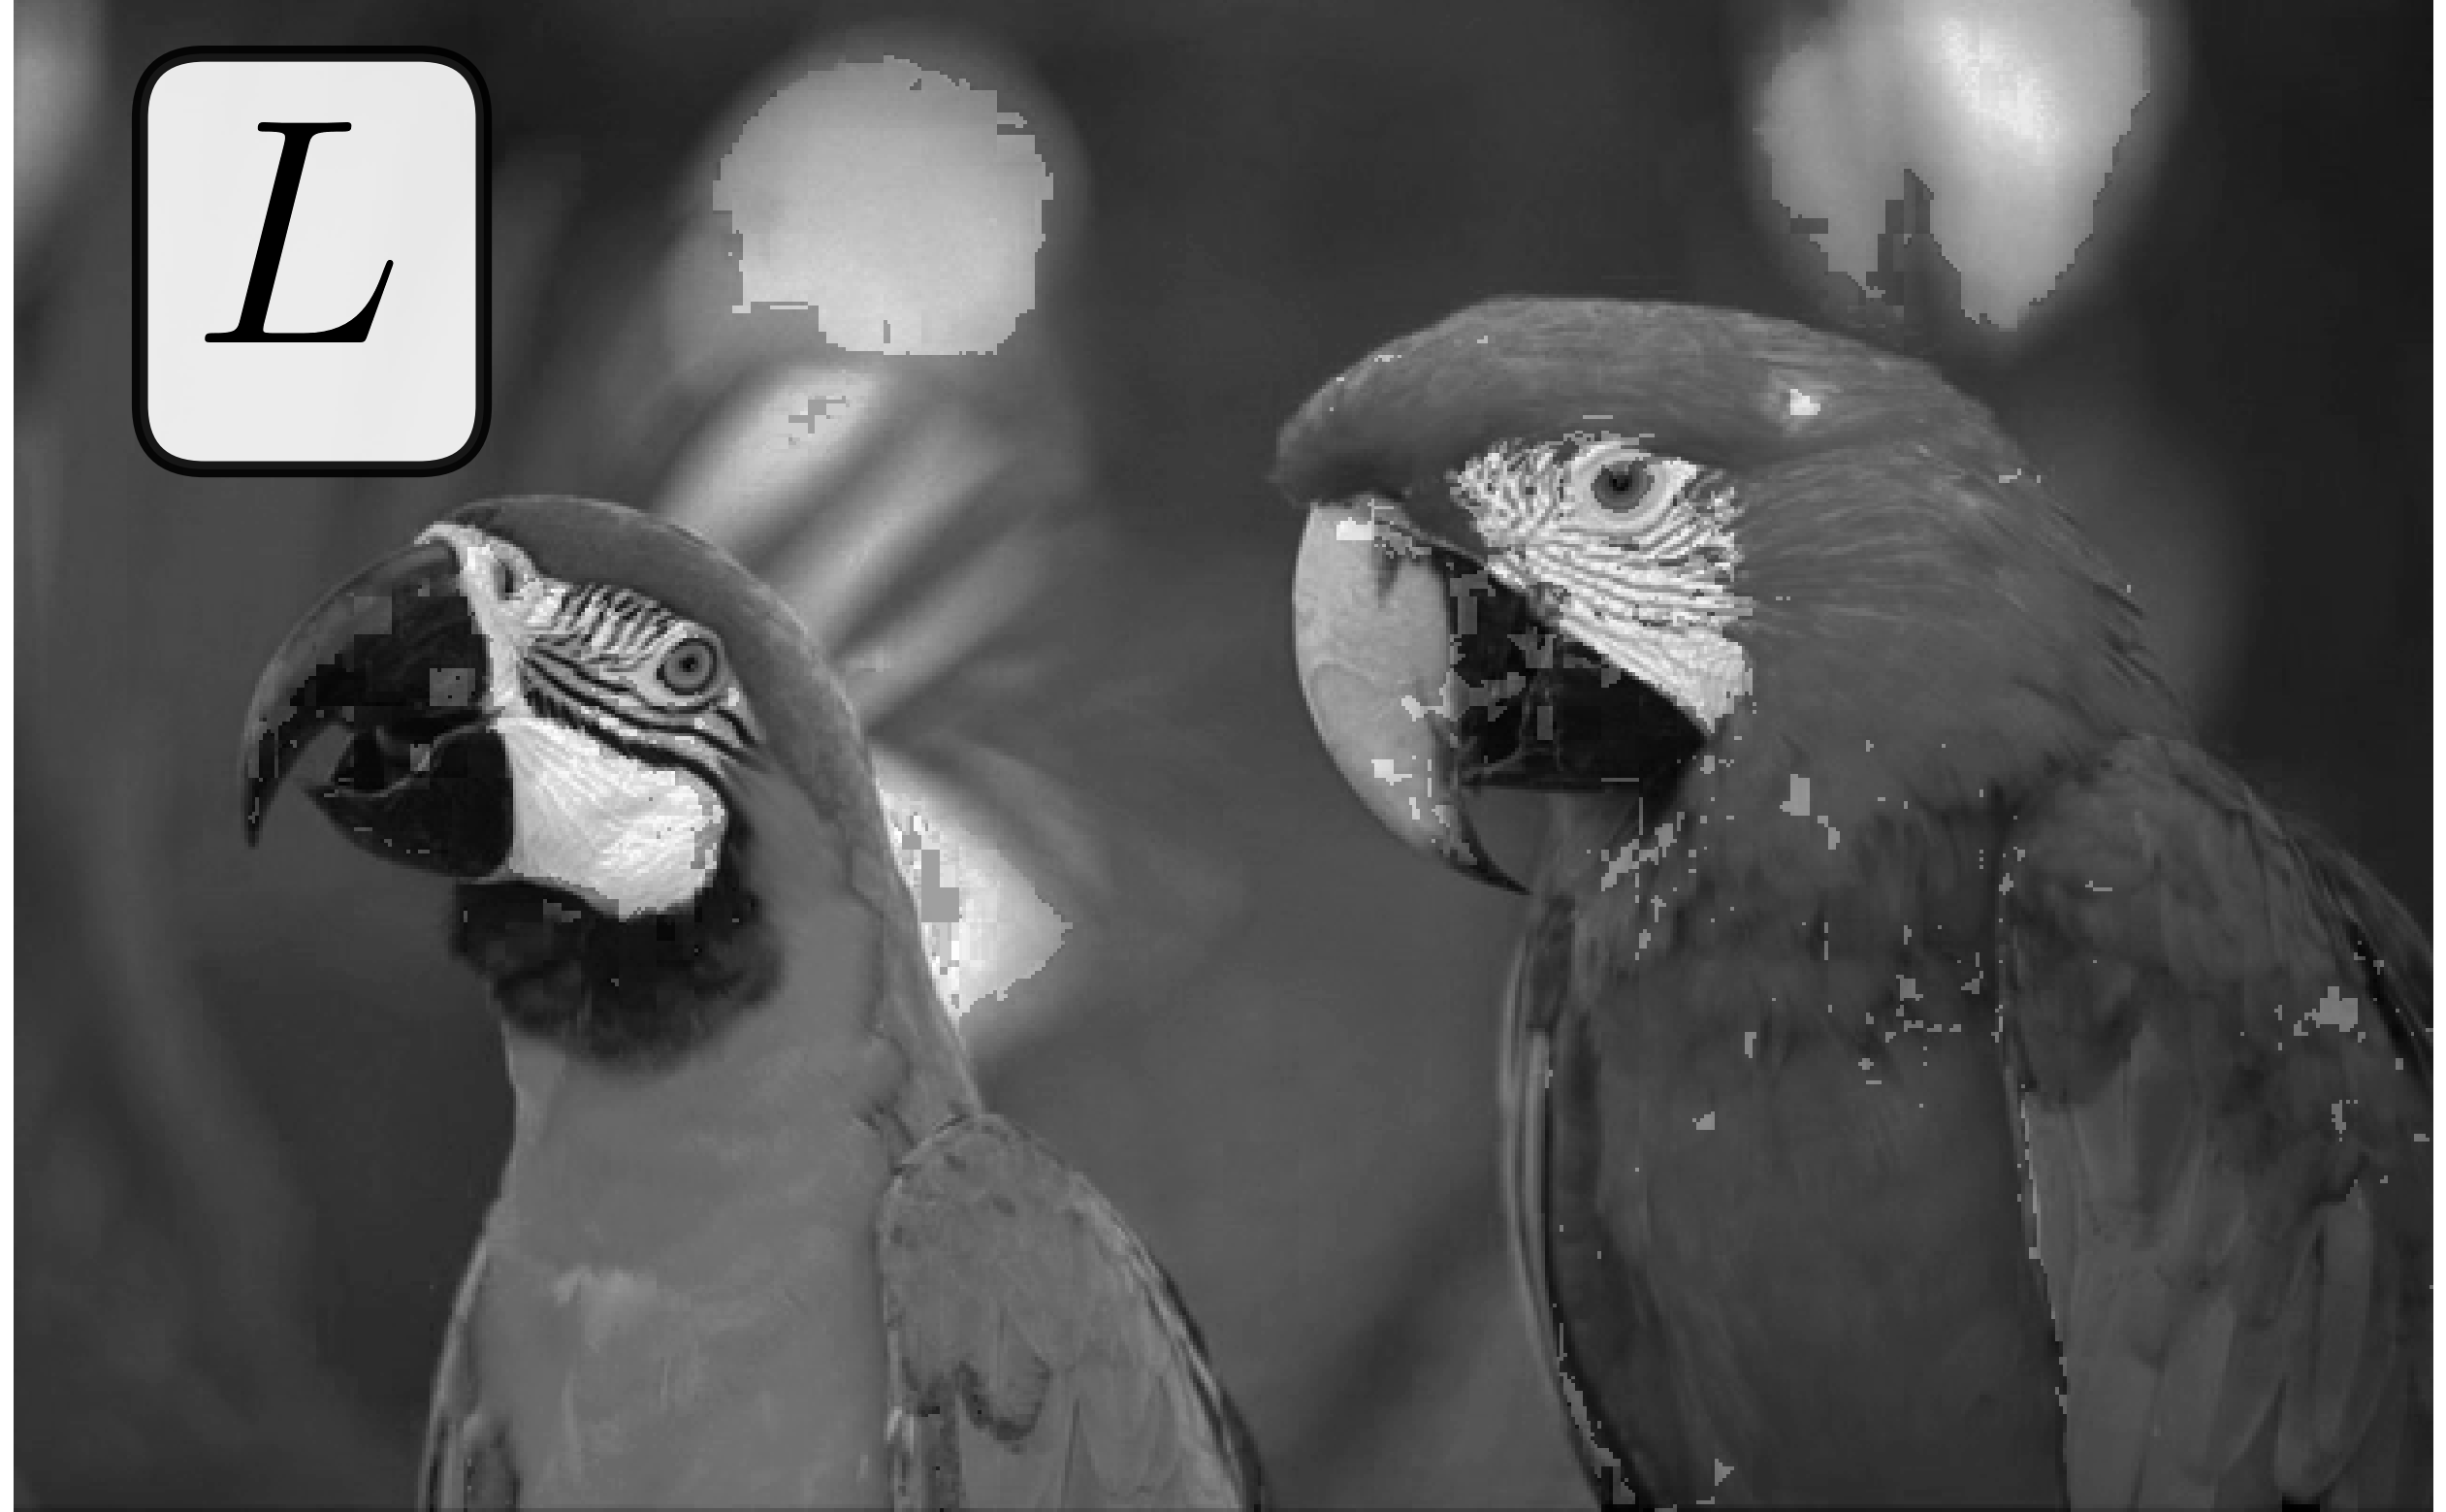
\includegraphics[width=\dimexpr\linewidth-20pt\relax]{araras_lum_HSV}
    \end{subfigure}      
    ~ %add desired spacing between images, e. g. ~, \quad, \qquad, \hfill etc. 
      %(or a blank line to force the subfigure onto a new line)
    \begin{subfigure}[b]{0.3\textwidth}
        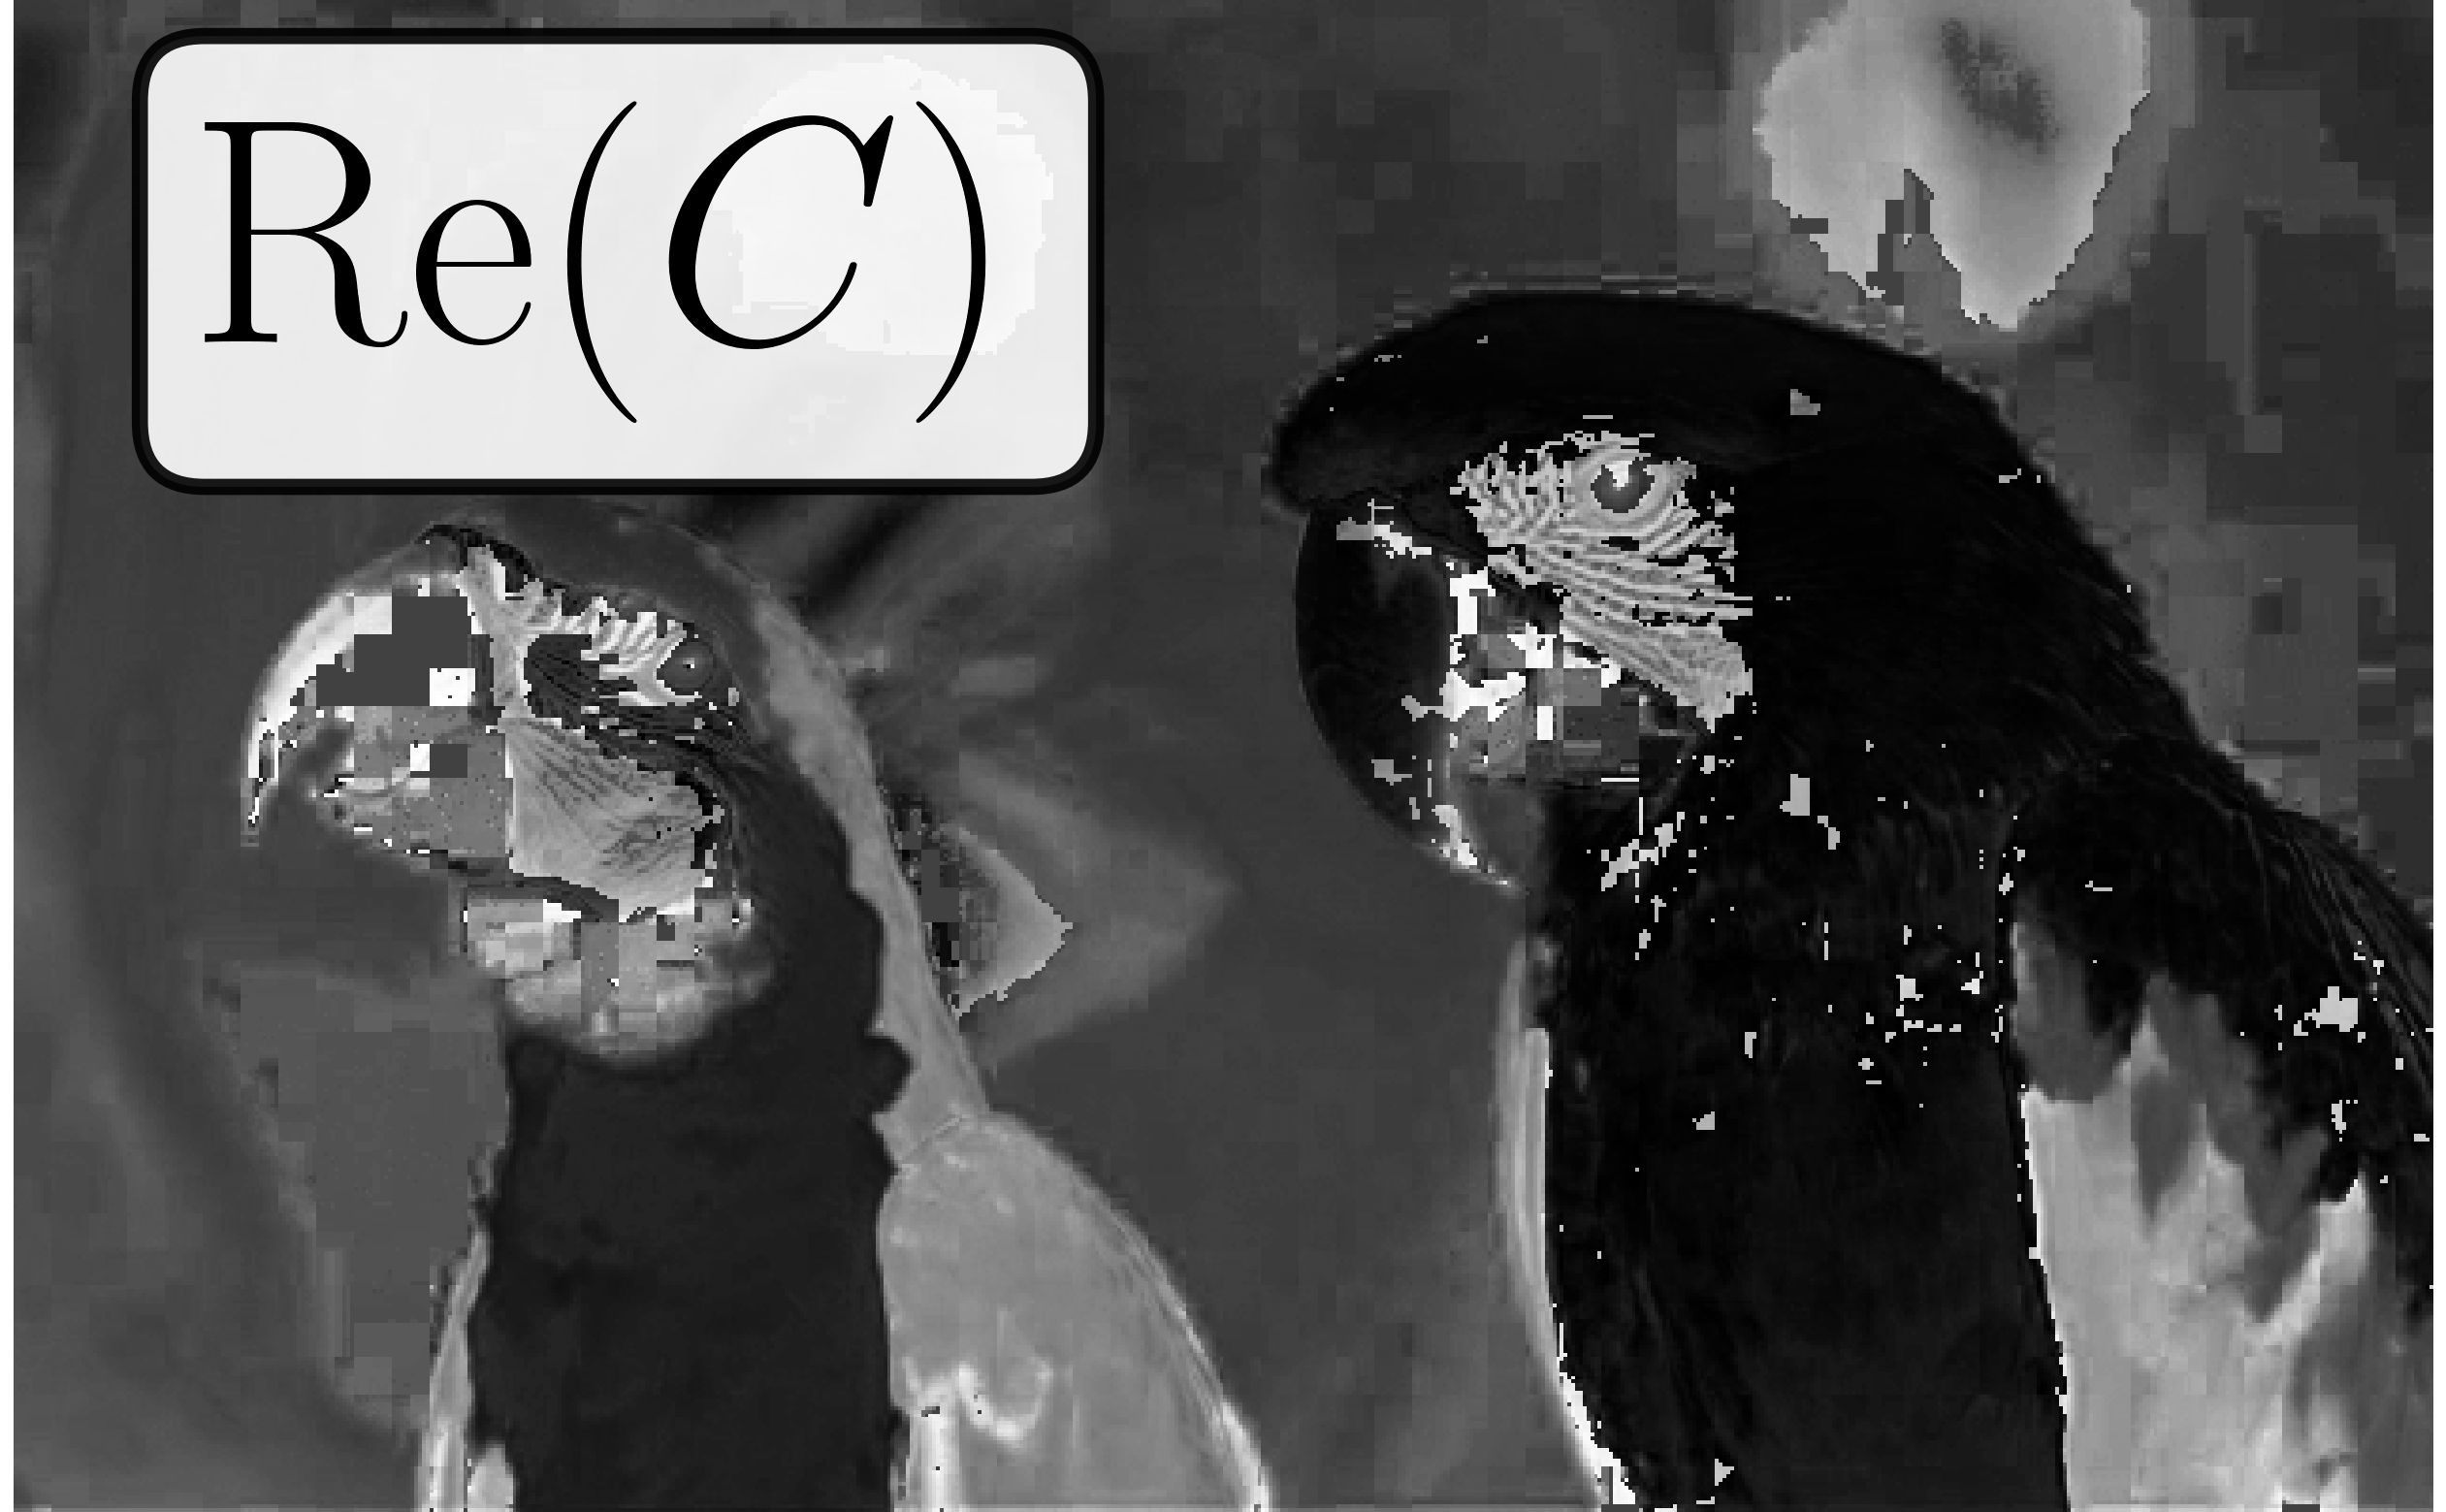
\includegraphics[width=\textwidth]{araras_chrr_HSV}
    \end{subfigure}
    ~ %add desired spacing between images, e. g. ~, \quad, \qquad, \hfill etc. 
      %(or a blank line to force the subfigure onto a new line)
    \begin{subfigure}[b]{0.3\textwidth}
        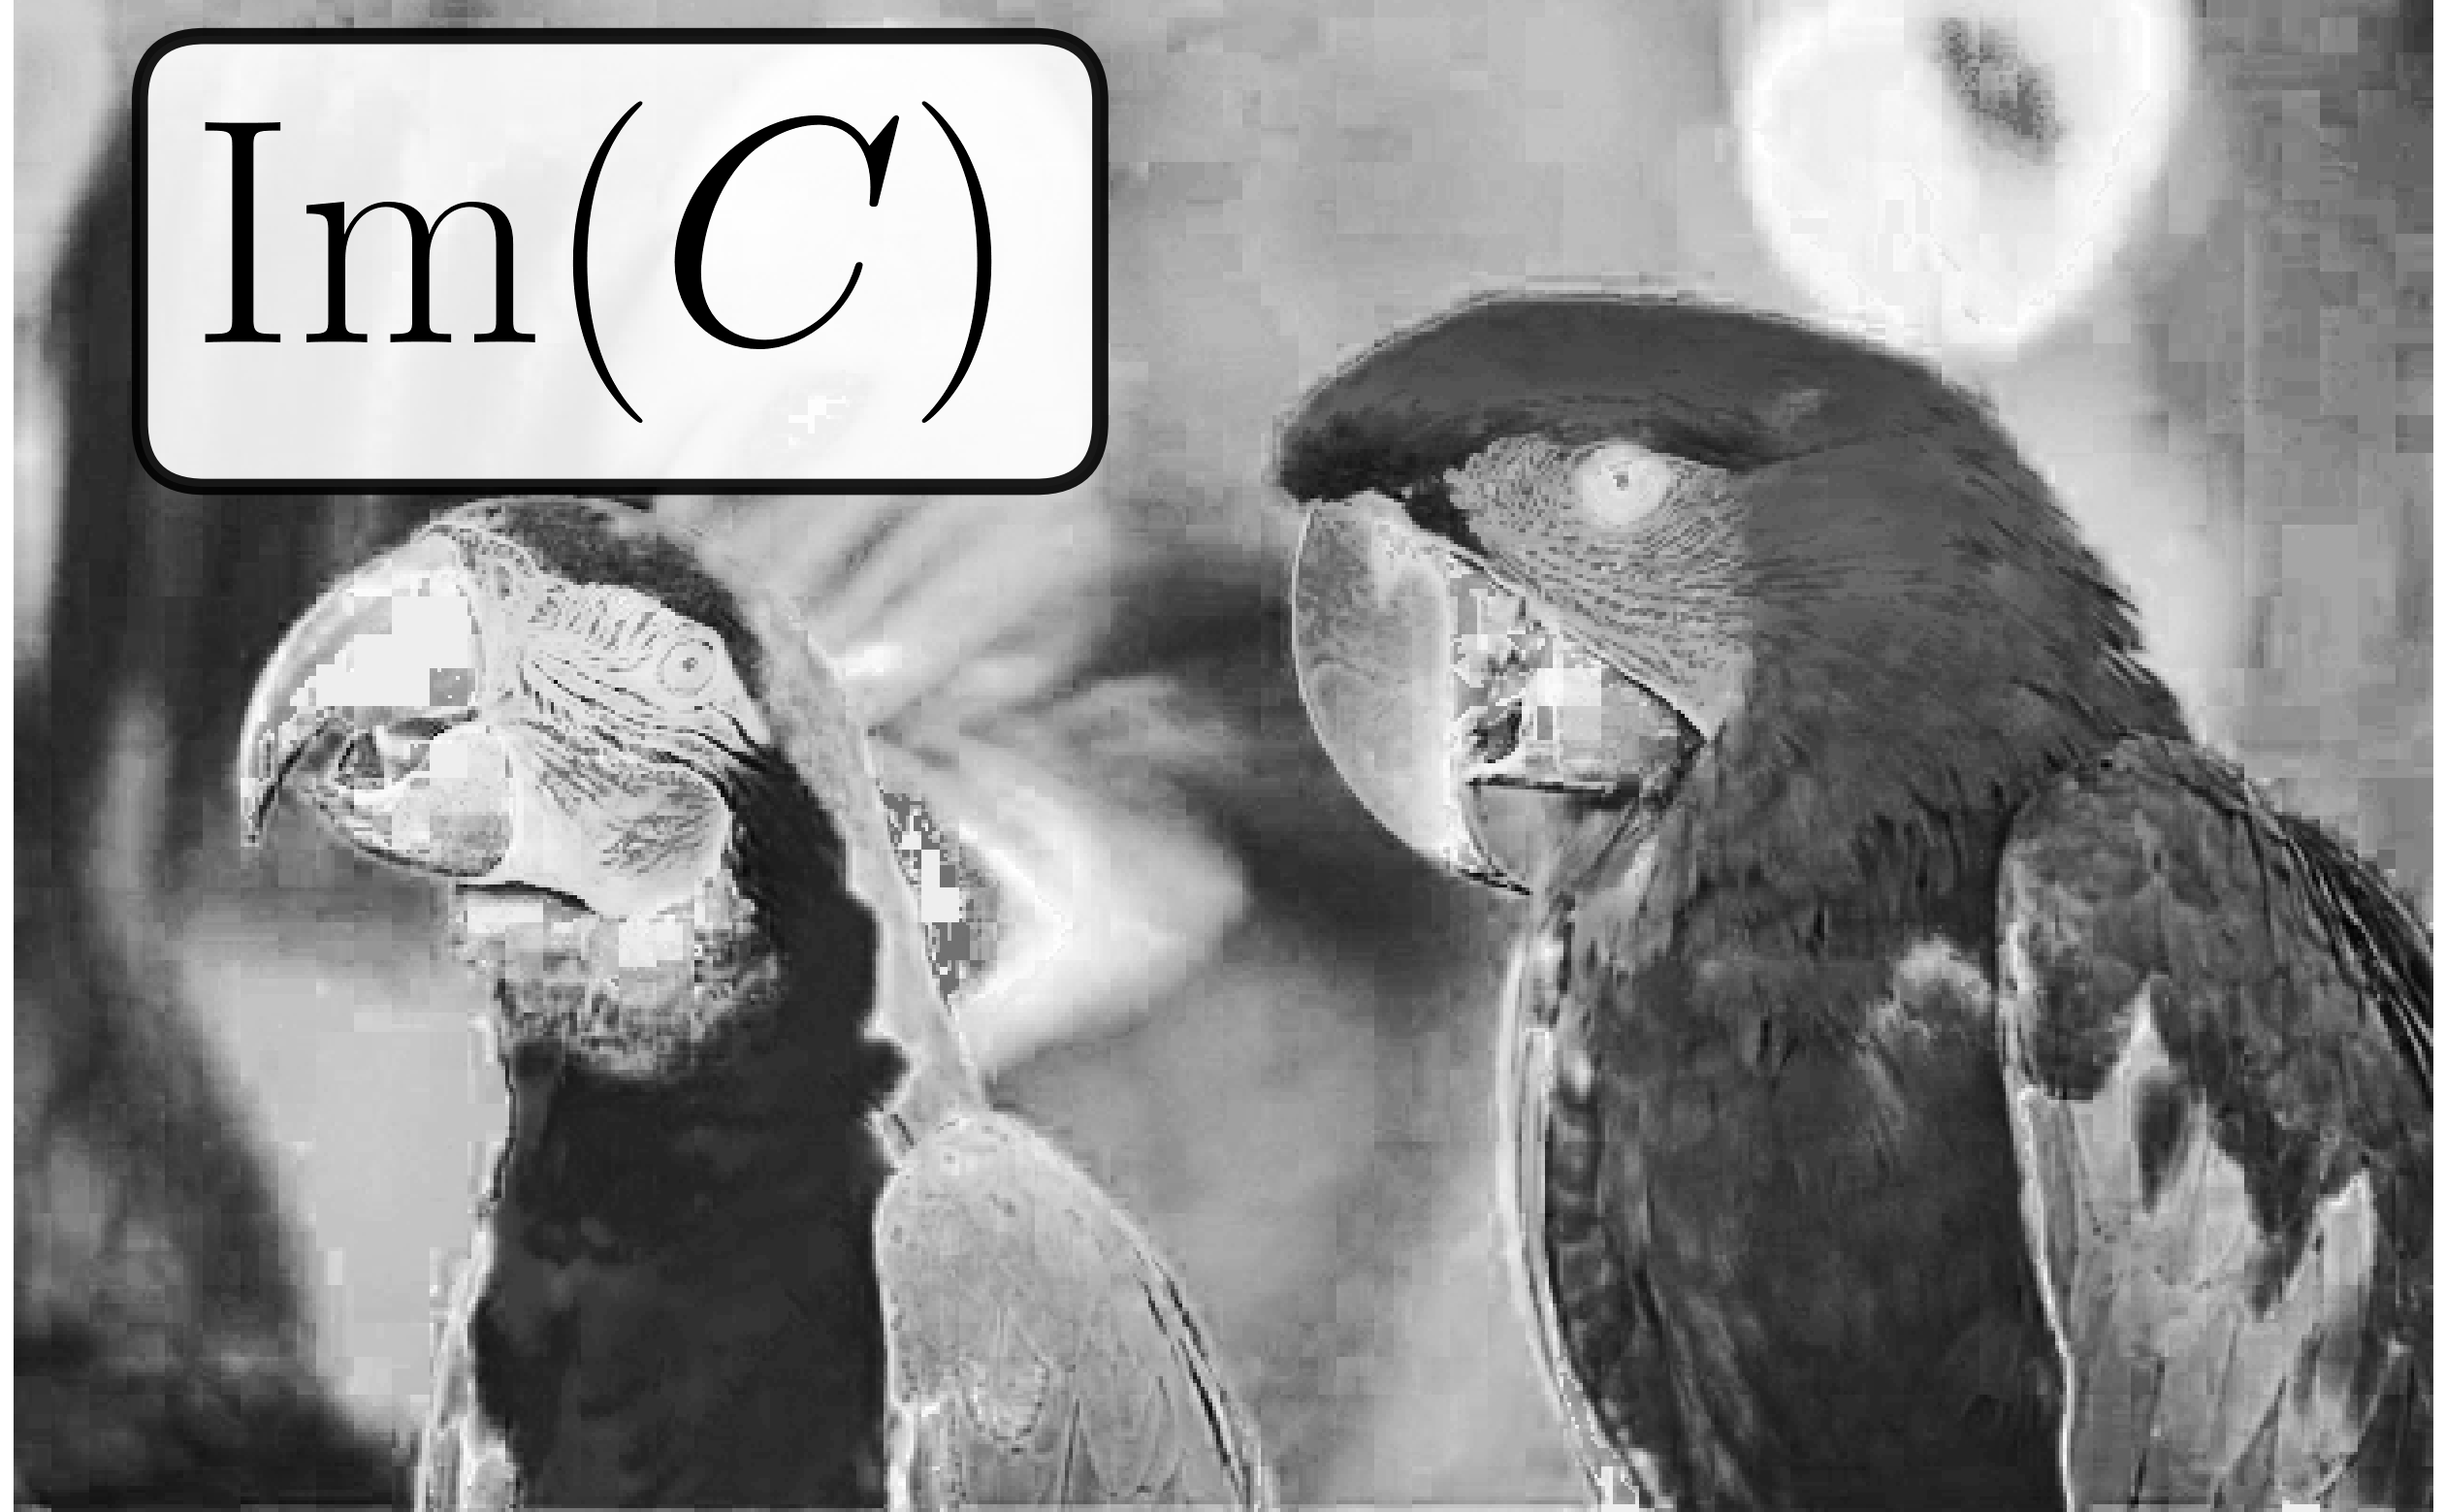
\includegraphics[width=\textwidth]{araras_chri_HSV}
    \end{subfigure} \vspace{5pt}      
    
    \begin{subfigure}[t]{\dimexpr0.3\textwidth+20pt\relax}
    	\makebox[20pt]{\raisebox{35pt}{ \rotatebox[origin=c]{90} {\small \textsf{\textbf{HSL luma/chroma}}} }}%
    	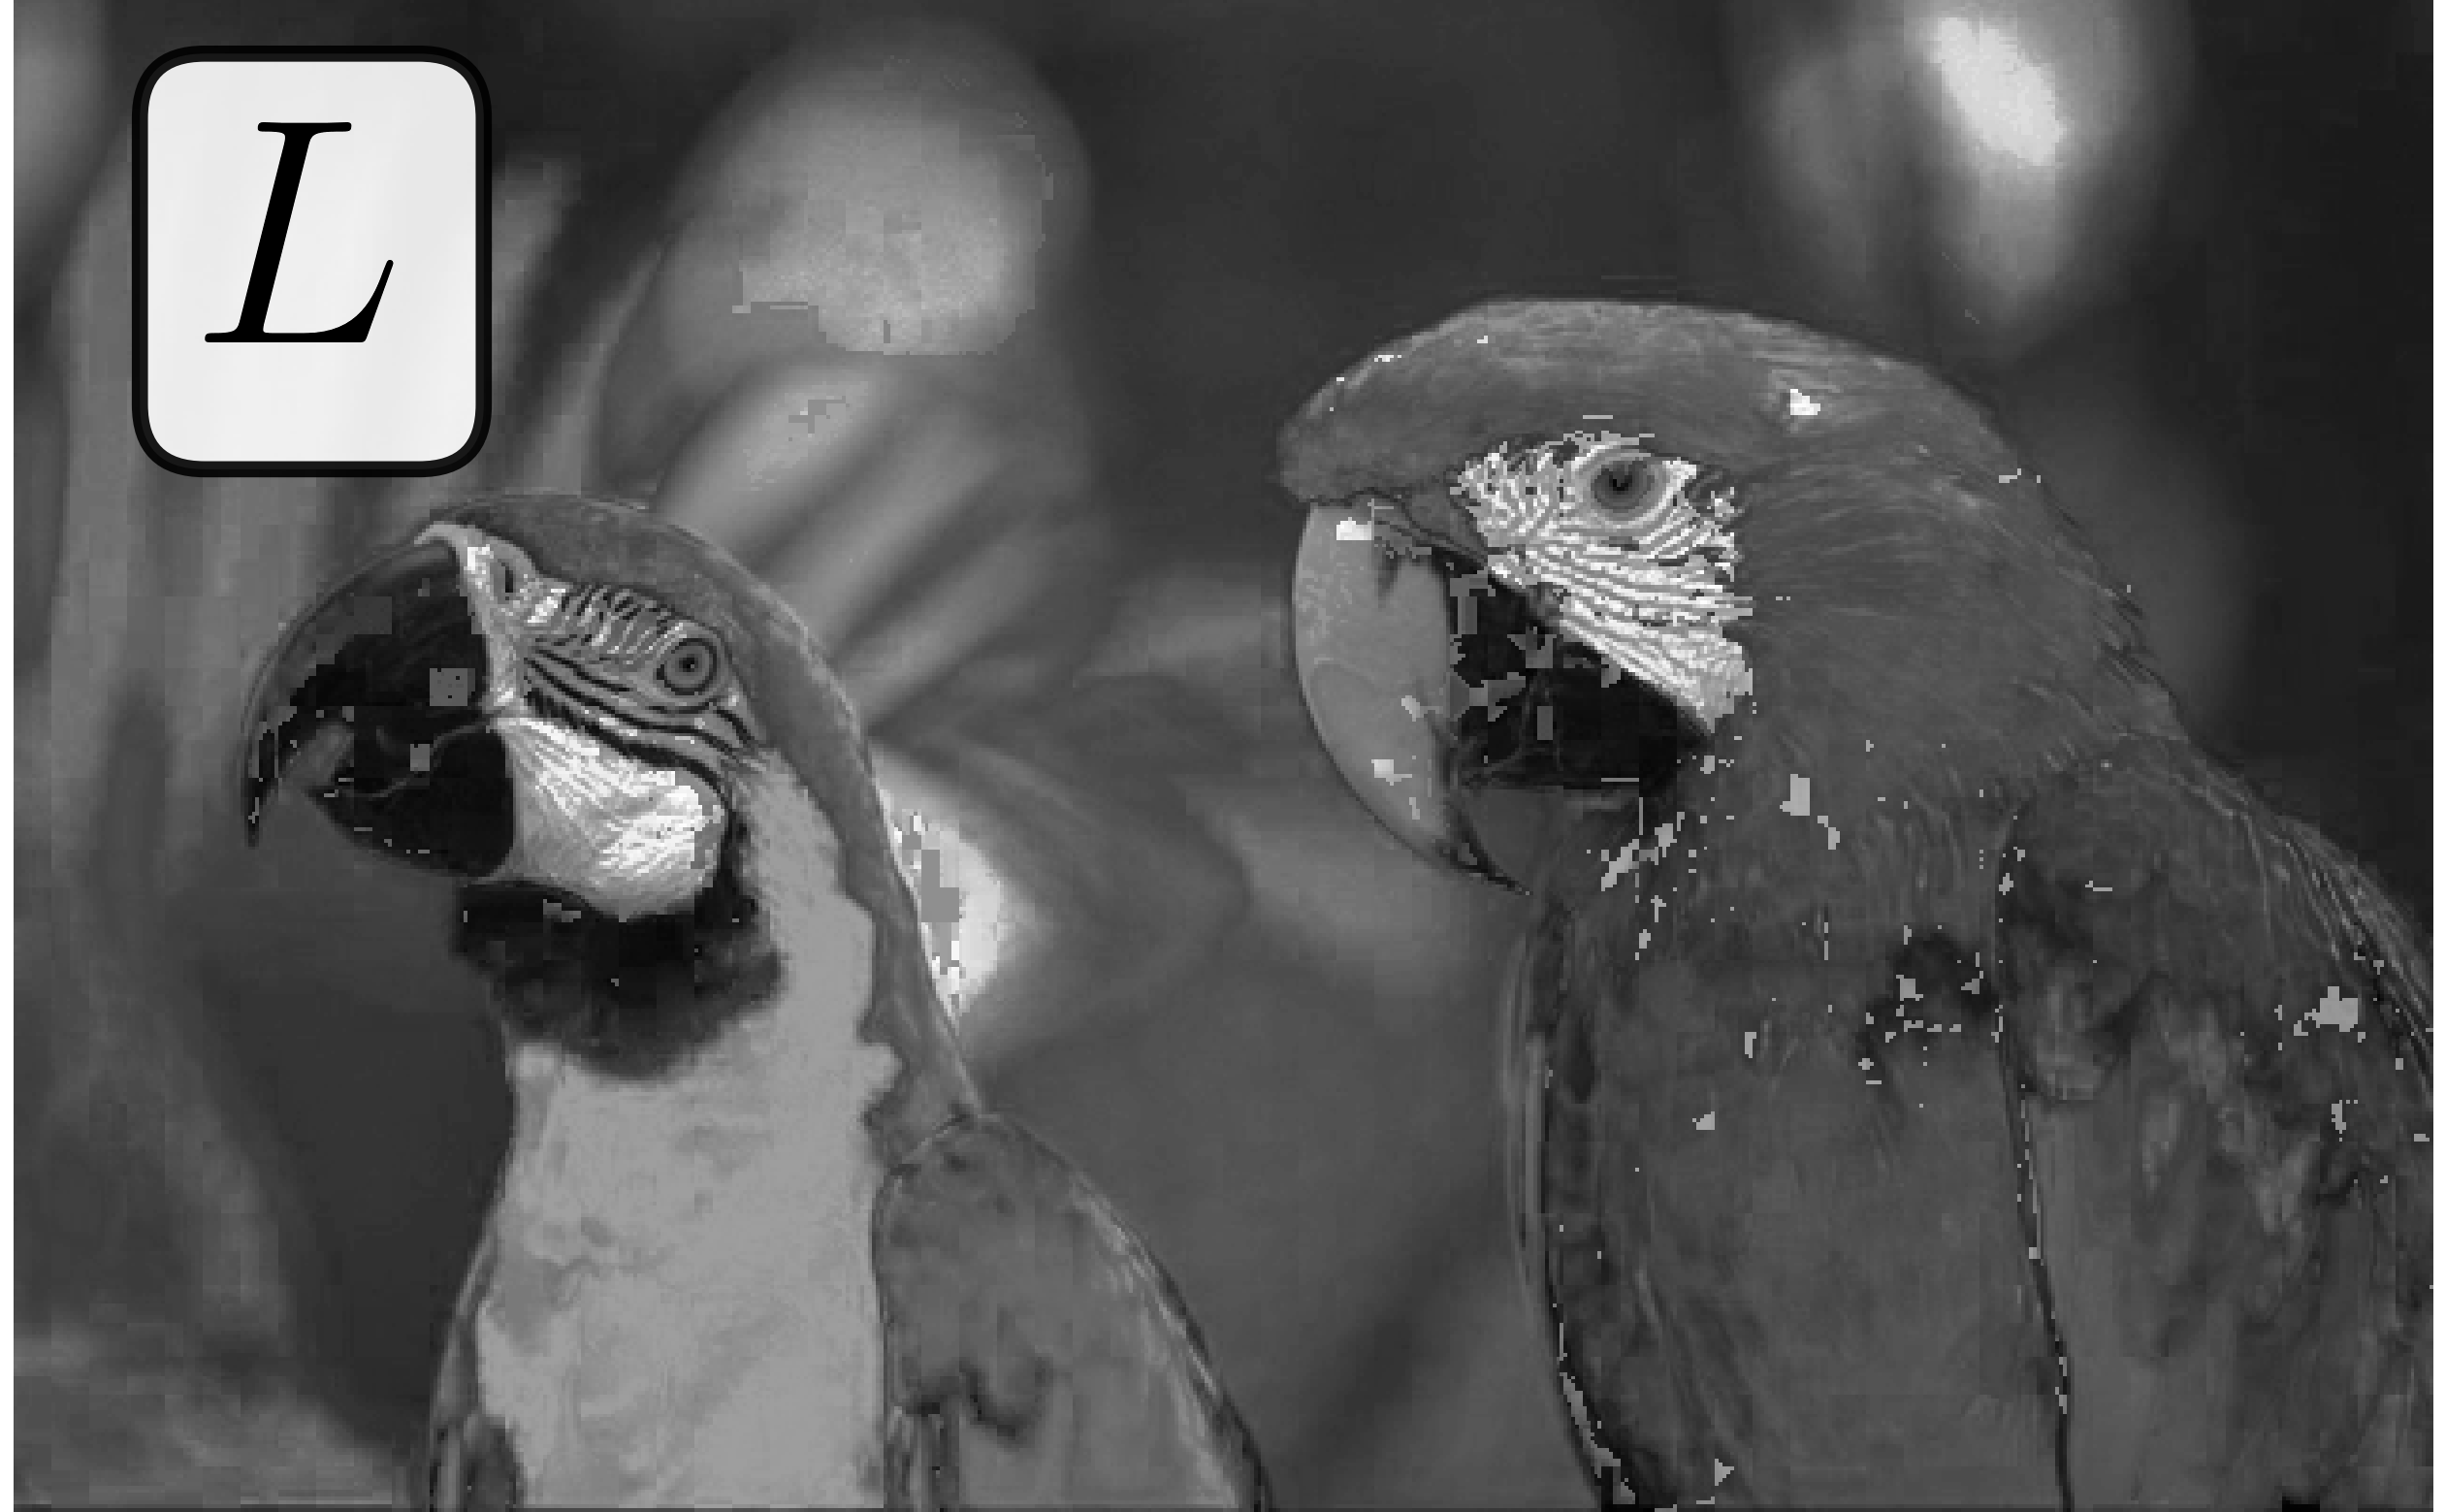
\includegraphics[width=\dimexpr\linewidth-20pt\relax]{araras_lum_HLS}
    \end{subfigure}     
    ~ %add desired spacing between images, e. g. ~, \quad, \qquad, \hfill etc. 
      %(or a blank line to force the subfigure onto a new line)
    \begin{subfigure}[b]{0.3\textwidth}
        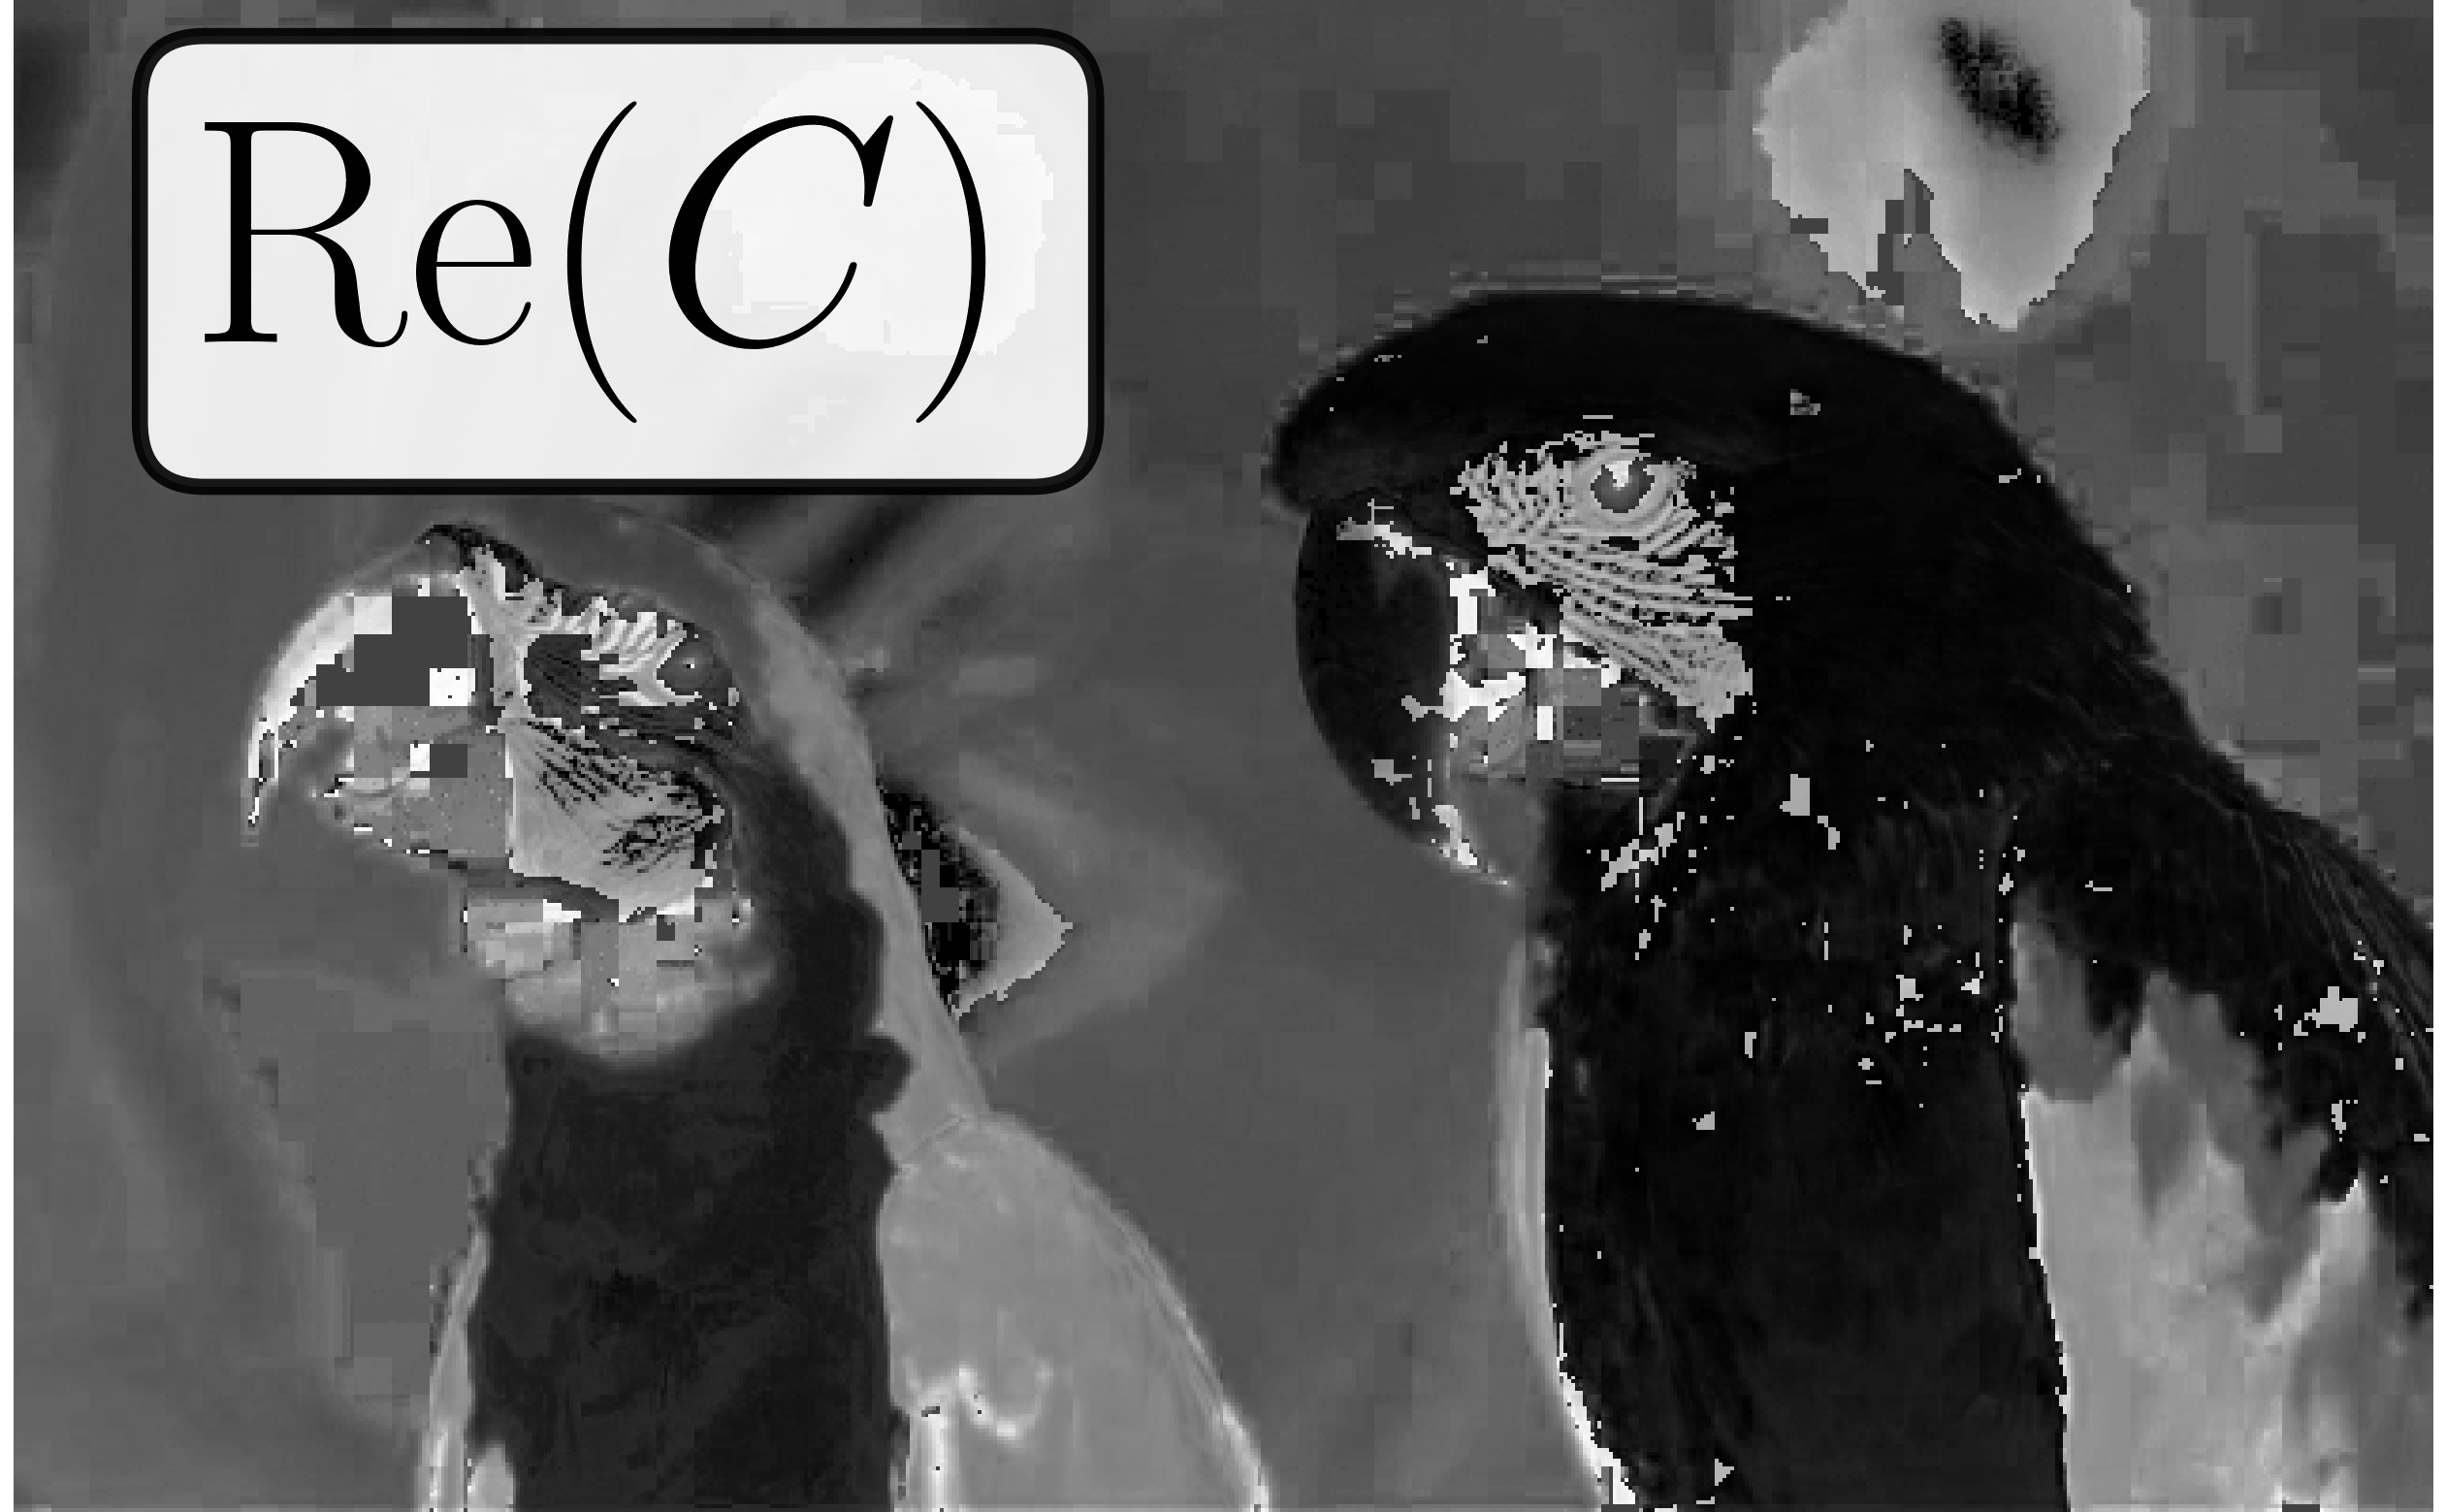
\includegraphics[width=\textwidth]{araras_chrr_HLS}
    \end{subfigure}
    ~ %add desired spacing between images, e. g. ~, \quad, \qquad, \hfill etc. 
      %(or a blank line to force the subfigure onto a new line)
    \begin{subfigure}[b]{0.3\textwidth}
        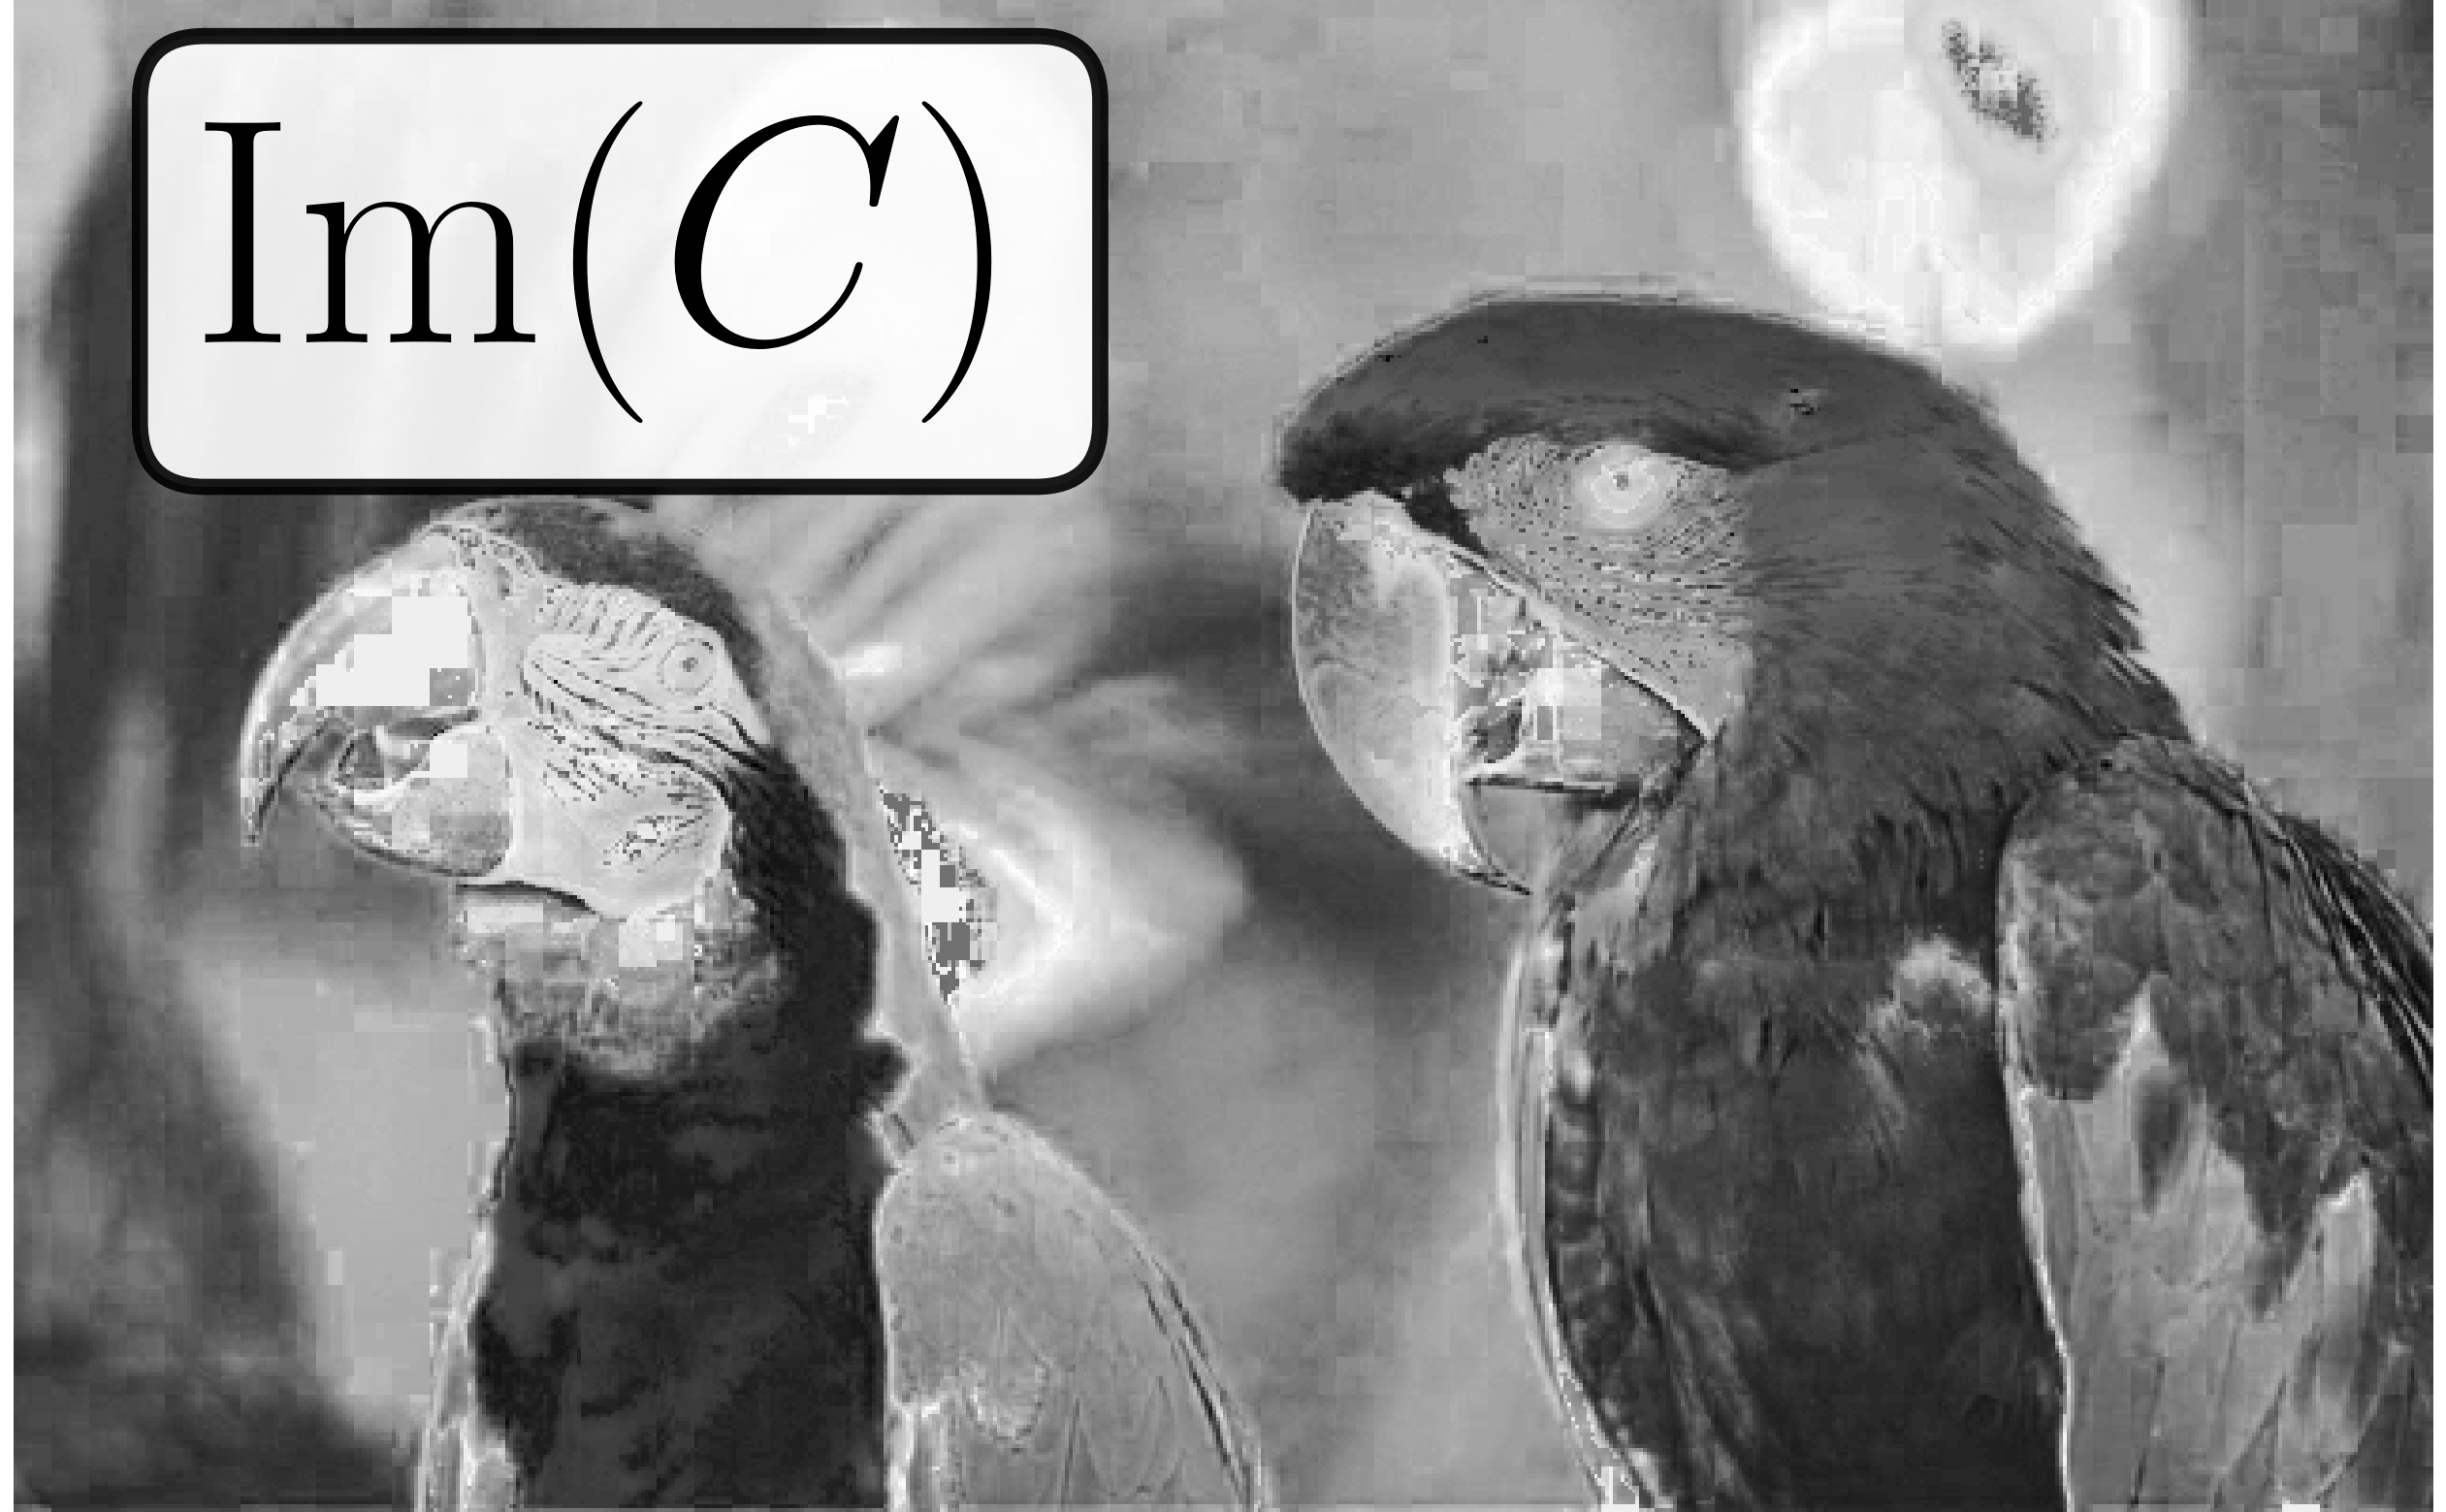
\includegraphics[width=\textwidth]{araras_chri_HLS}
    \end{subfigure} \vspace{5pt} 
    
    \begin{subfigure}[t]{\dimexpr0.3\textwidth+20pt\relax}
    	\makebox[20pt]{\raisebox{35pt}{ \rotatebox[origin=c]{90} {\small \textsf{\textbf{LAB luma/chroma}}} }}%
    	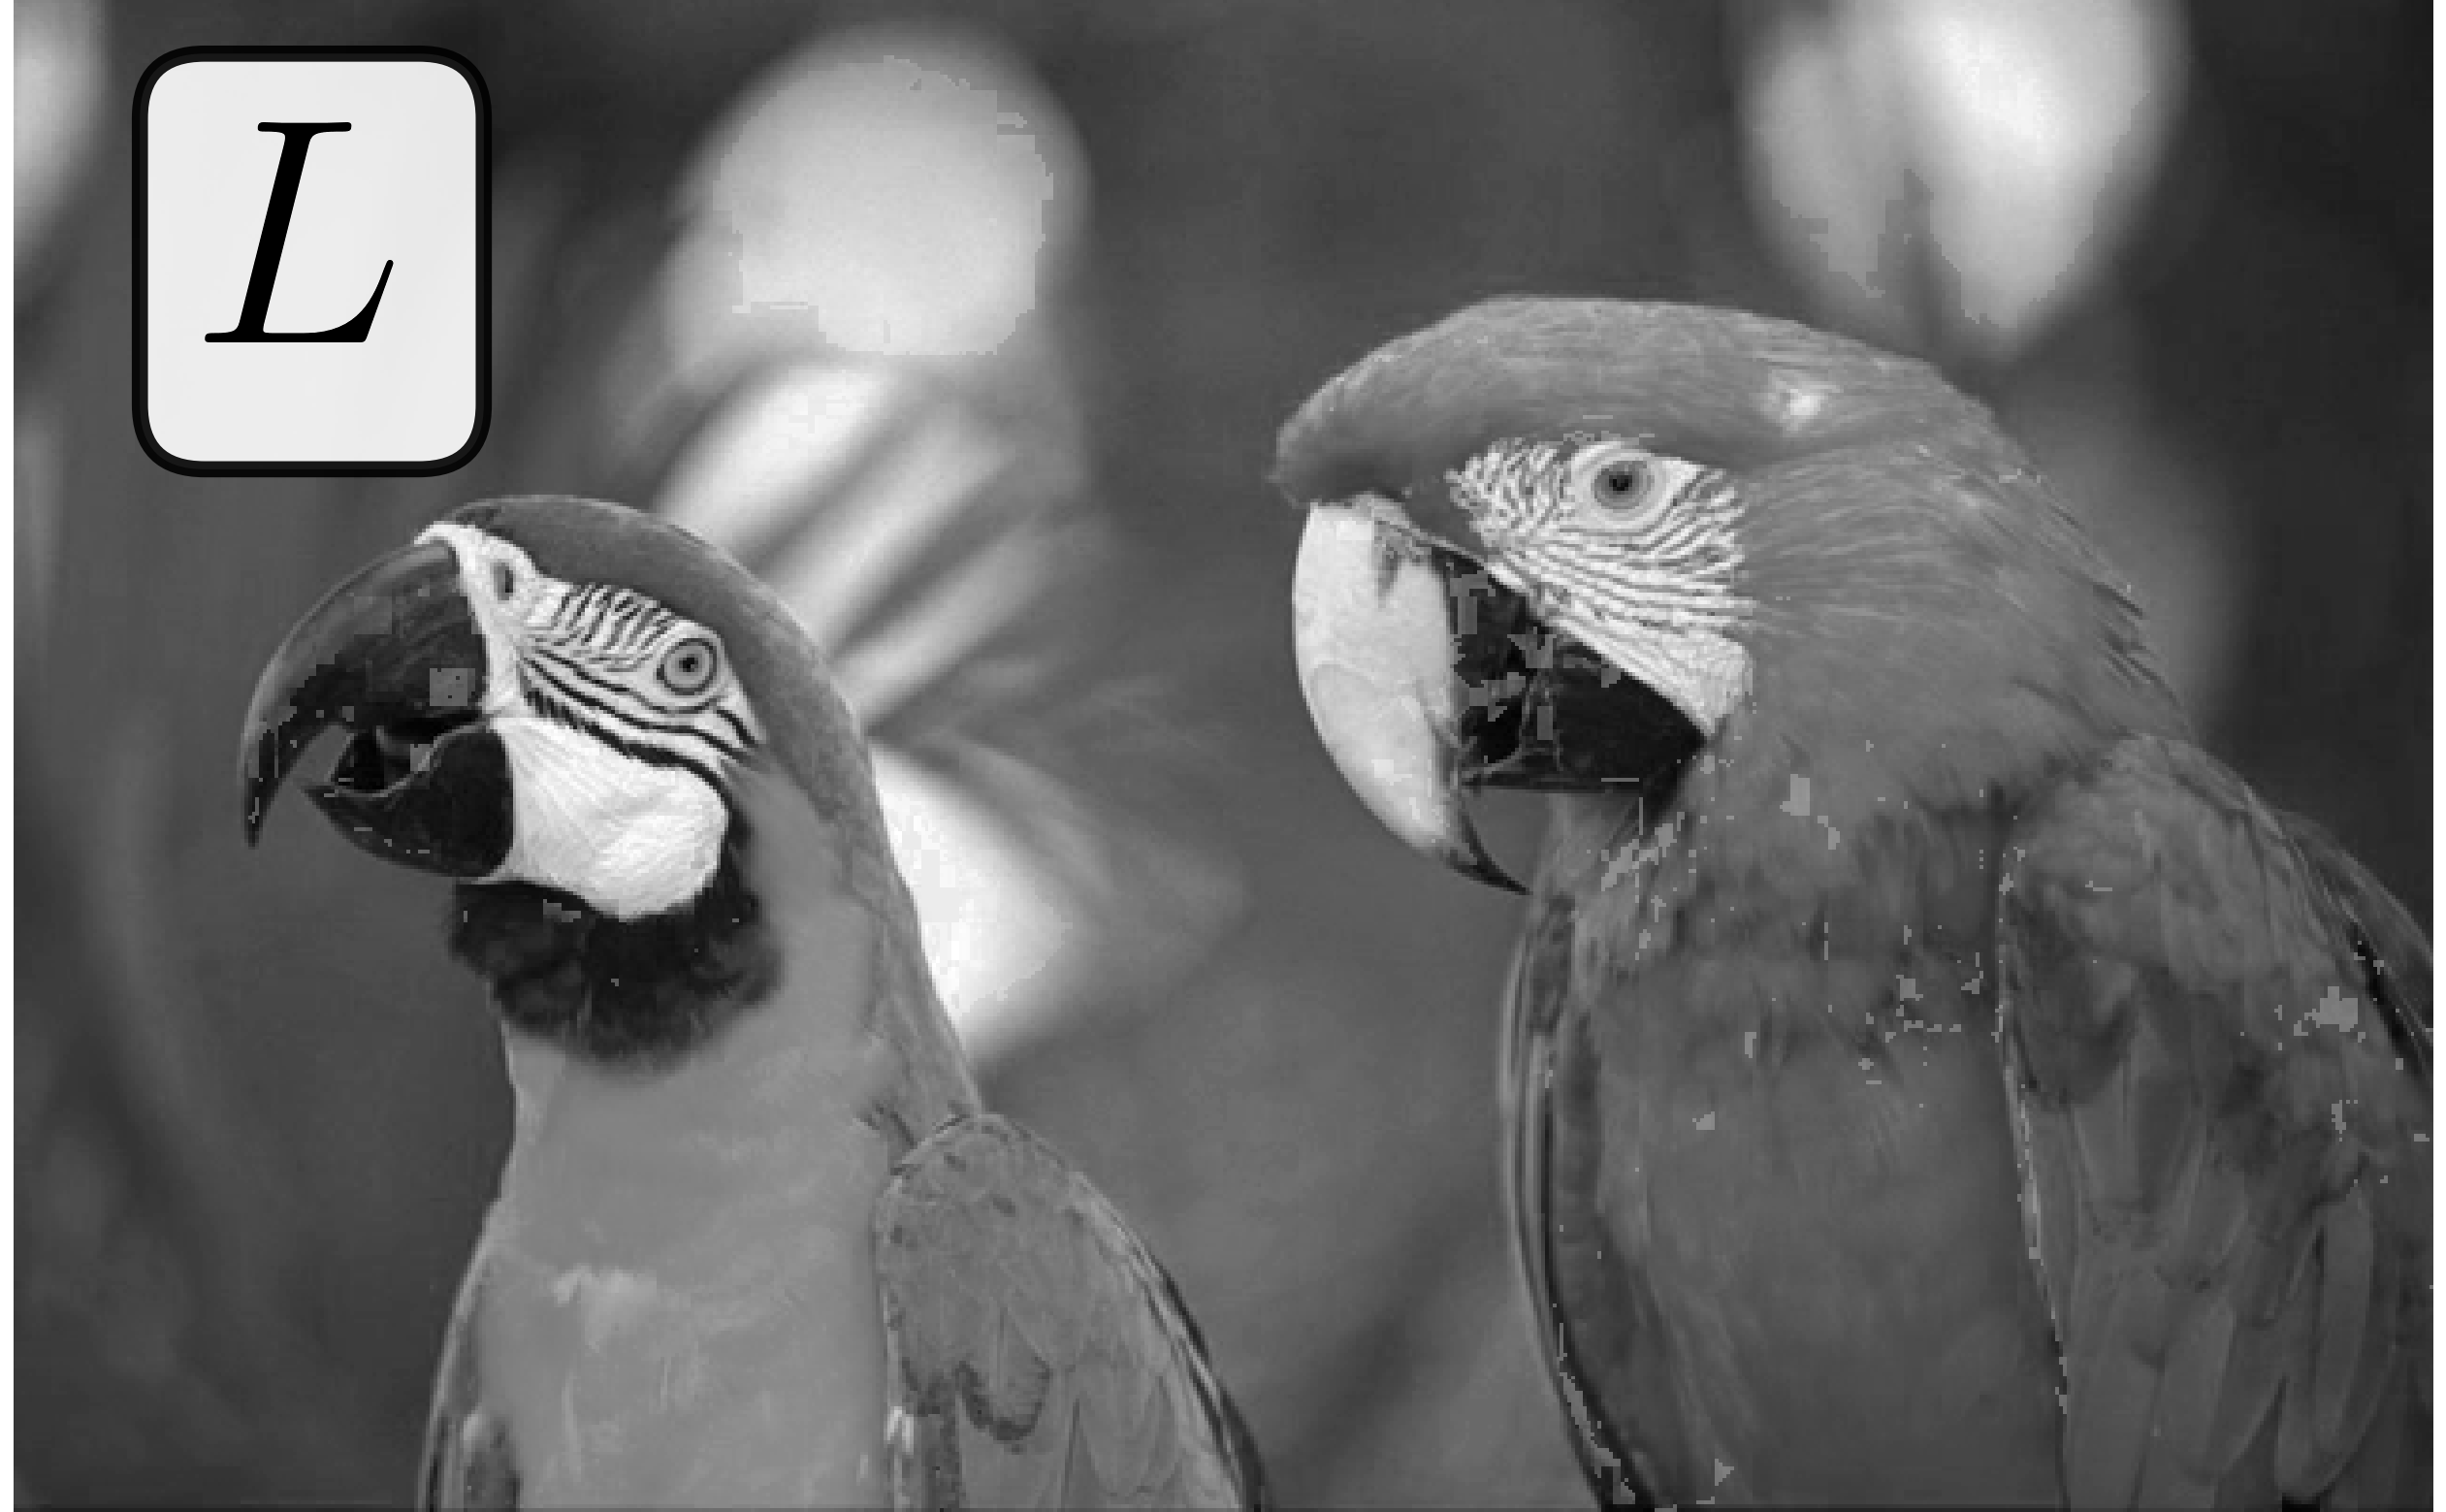
\includegraphics[width=\dimexpr\linewidth-20pt\relax]{araras_lum_LAB}
    \end{subfigure}     
    ~ %add desired spacing between images, e. g. ~, \quad, \qquad, \hfill etc. 
      %(or a blank line to force the subfigure onto a new line)
    \begin{subfigure}[b]{0.3\textwidth}
        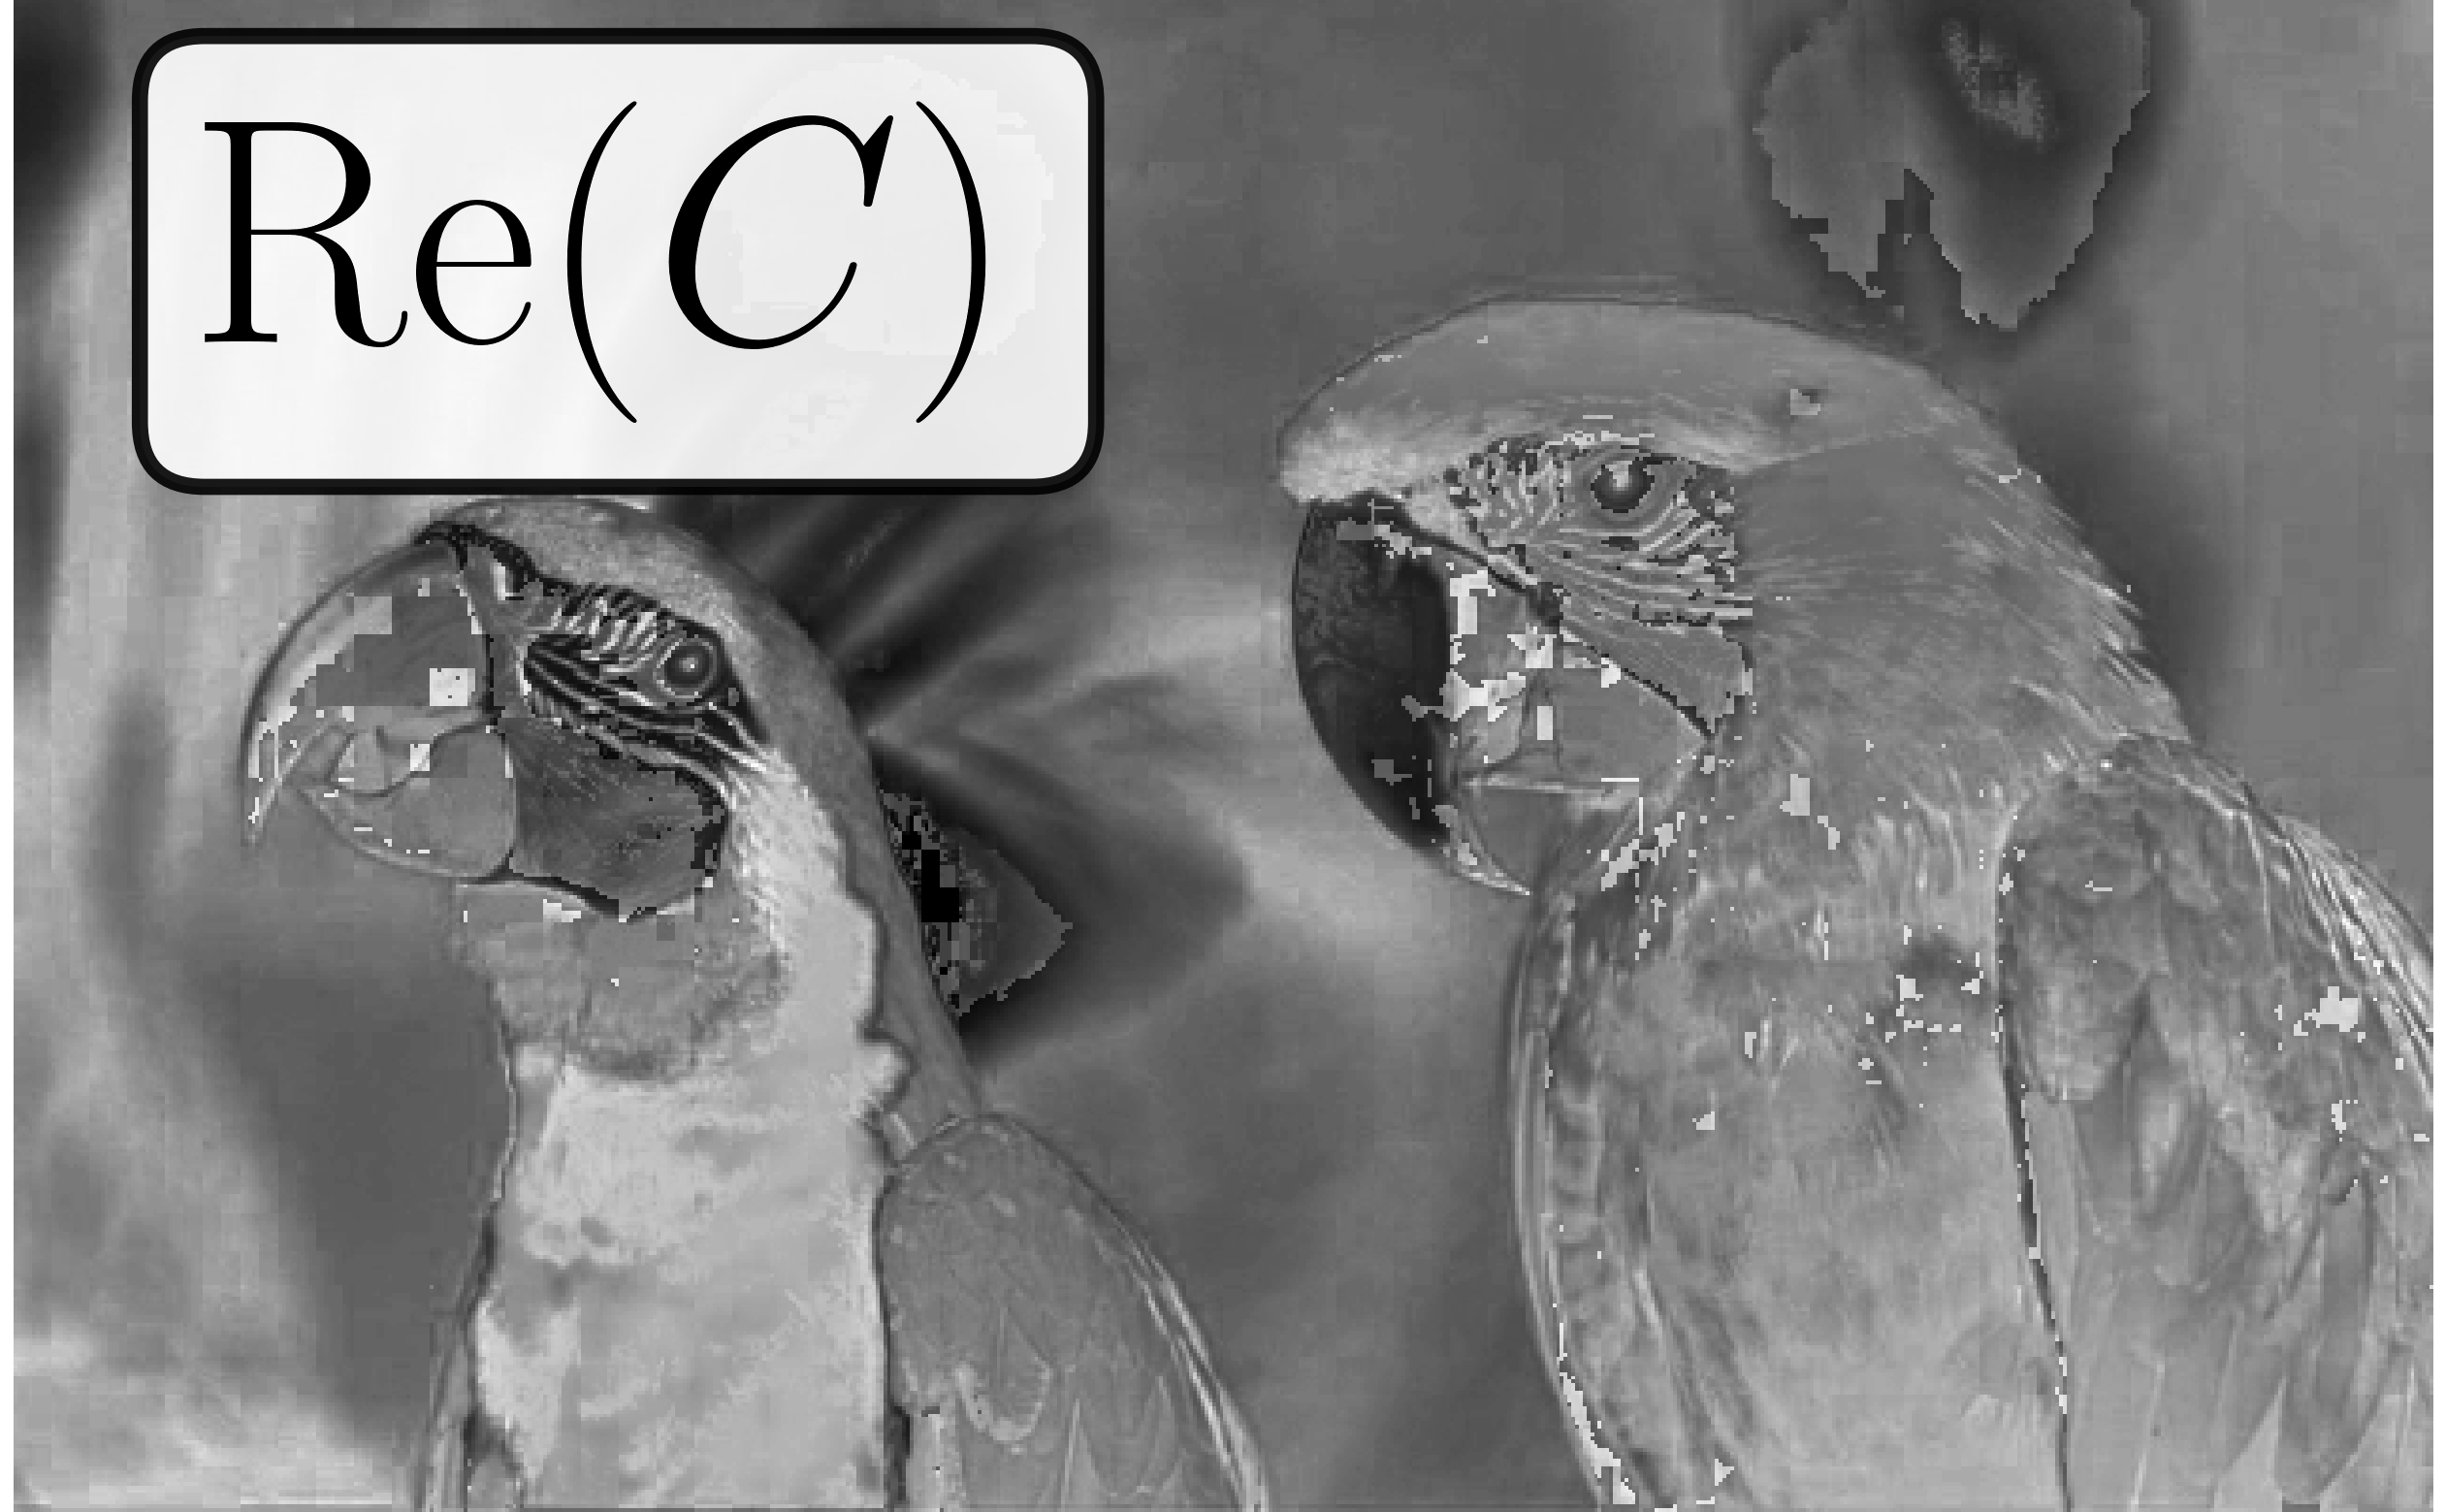
\includegraphics[width=\textwidth]{araras_chrr_LAB}
    \end{subfigure}
    ~ %add desired spacing between images, e. g. ~, \quad, \qquad, \hfill etc. 
      %(or a blank line to force the subfigure onto a new line)
    \begin{subfigure}[b]{0.3\textwidth}
        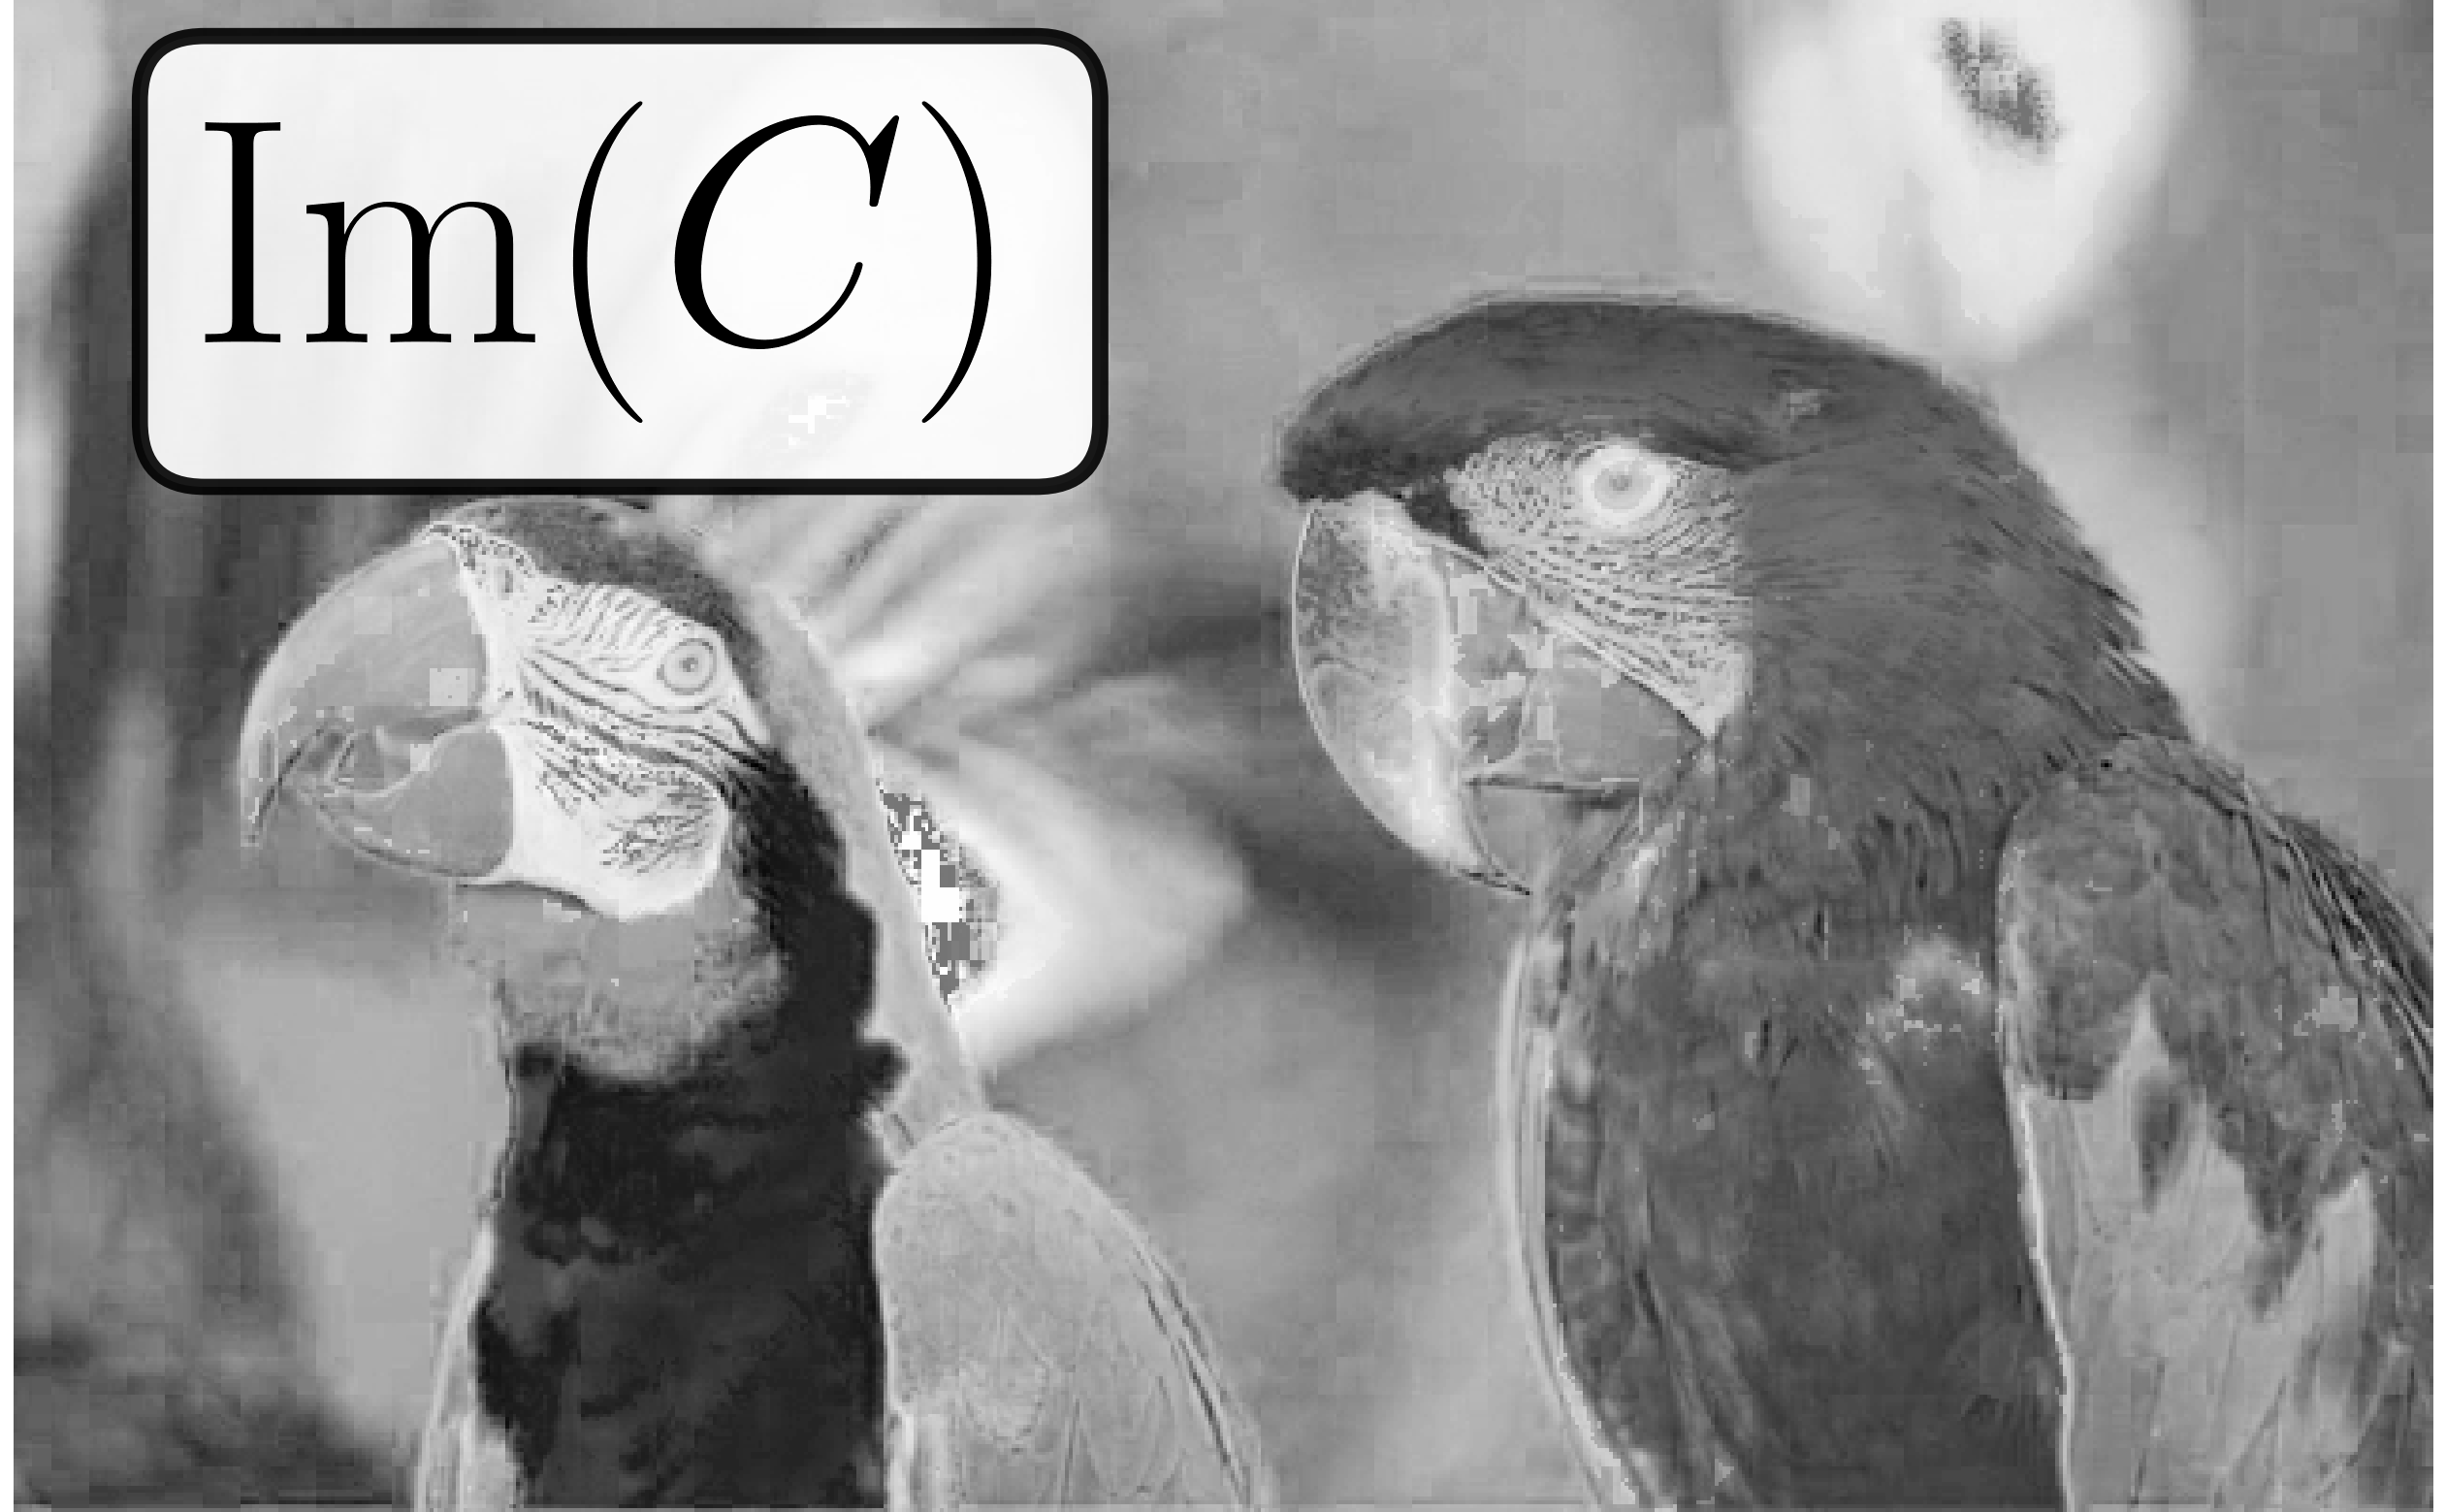
\includegraphics[width=\textwidth]{araras_chri_LAB}
    \end{subfigure} \vspace{5pt} 
        
    \caption{Color channels of an image in different color spaces in grayscale}\label{fig:images_color_complex_space}    
\end{figure}

Figure \ref{fig:images_color_complex_space} shows the transformation of a natural image (first row of the figure array) from RGB space to complex two-channel color space. Each row in the figure shows the luminance channel and the two parts (real and imaginary) of the chrominance channel. Note that as it happened in the representation of the classic color spaces (figure \ref{fig:images_color_space}), since the method of computing saturation differs in HSV and HSL spaces, the chrominance channel is different. The same effect occurs with the L lumance channel from LAB space and the luminance from the RGB to gray transformation; in theory both are the same, but in practice we can see that there are differences.


%From the previous section, it is clear that the luminance information is a cue in obtaining texture features, however, the chrominance also plays an important role. We can obtain this information using the two-complex channels form. This representation contains the pure luminance $L^*$ values in a real channel while the chrominance $C$ is contained in a complex channel. This complex channel can be obtained from the components of the $L^*a^*b^*$ or the components of $HSV$ / $HSL$ color spaces prior to a transformation of the image from the $RGB$ space.
%
%Thus, the complex chrominance channel in its exponential form is defined as  
%
%
%where $H$ is the hue and $S$ is the saturation value obtained after the $RGB$ to $HLS$ transformation. While the combined chrominance function for $L^*a^*b^*$ is defined as
%
%
%where $a^*$ and $b^*$ are two chroma variables obtained from $RGB$ to $L^*a^*b^*$ transformation. 
%
%We obtain a complex representation of chrominance content of the image whose spectrum is interesting to analyze in order to characterize the spatial variations of the chromatic part of the image. 


\subsection{Compact color representations for image processing}
The overall distribution of color within an image is a useful clue that contributes to the description of the content of an image. For example, we can characterize images that contain landscapes with mountains, jungles, urban environments, deserts or other scenes with different elements by their color distribution. The global color distribution can be represented by means of a color image histogram, which is a discrete function that associates to each intensity value (per color channel) the number of pixels that belong to this value.

The advantages of this representation is that they are invariant to the rotation or translation of the image, as well as, to a lesser extent, to changes of point of view and changes of scale. In addition, we can compact the image color information by reducing the count intervals, that is, by selecting a small number of bins.

\subsubsection{Single-channel Color Histogram}



\begin{figure}[!ht]
    \centering
    \begin{subfigure}[b]{0.45\textwidth}
        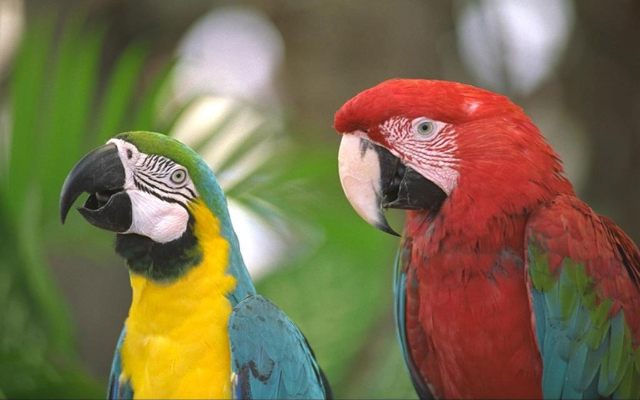
\includegraphics[width=\textwidth]{araras}
        \caption{Input image}
    \end{subfigure}
        ~ %add desired spacing between images, e. g. ~, \quad, \qquad, \hfill etc. 
      %(or a blank line to force the subfigure onto a new line)
    \begin{subfigure}[b]{0.45\textwidth}
        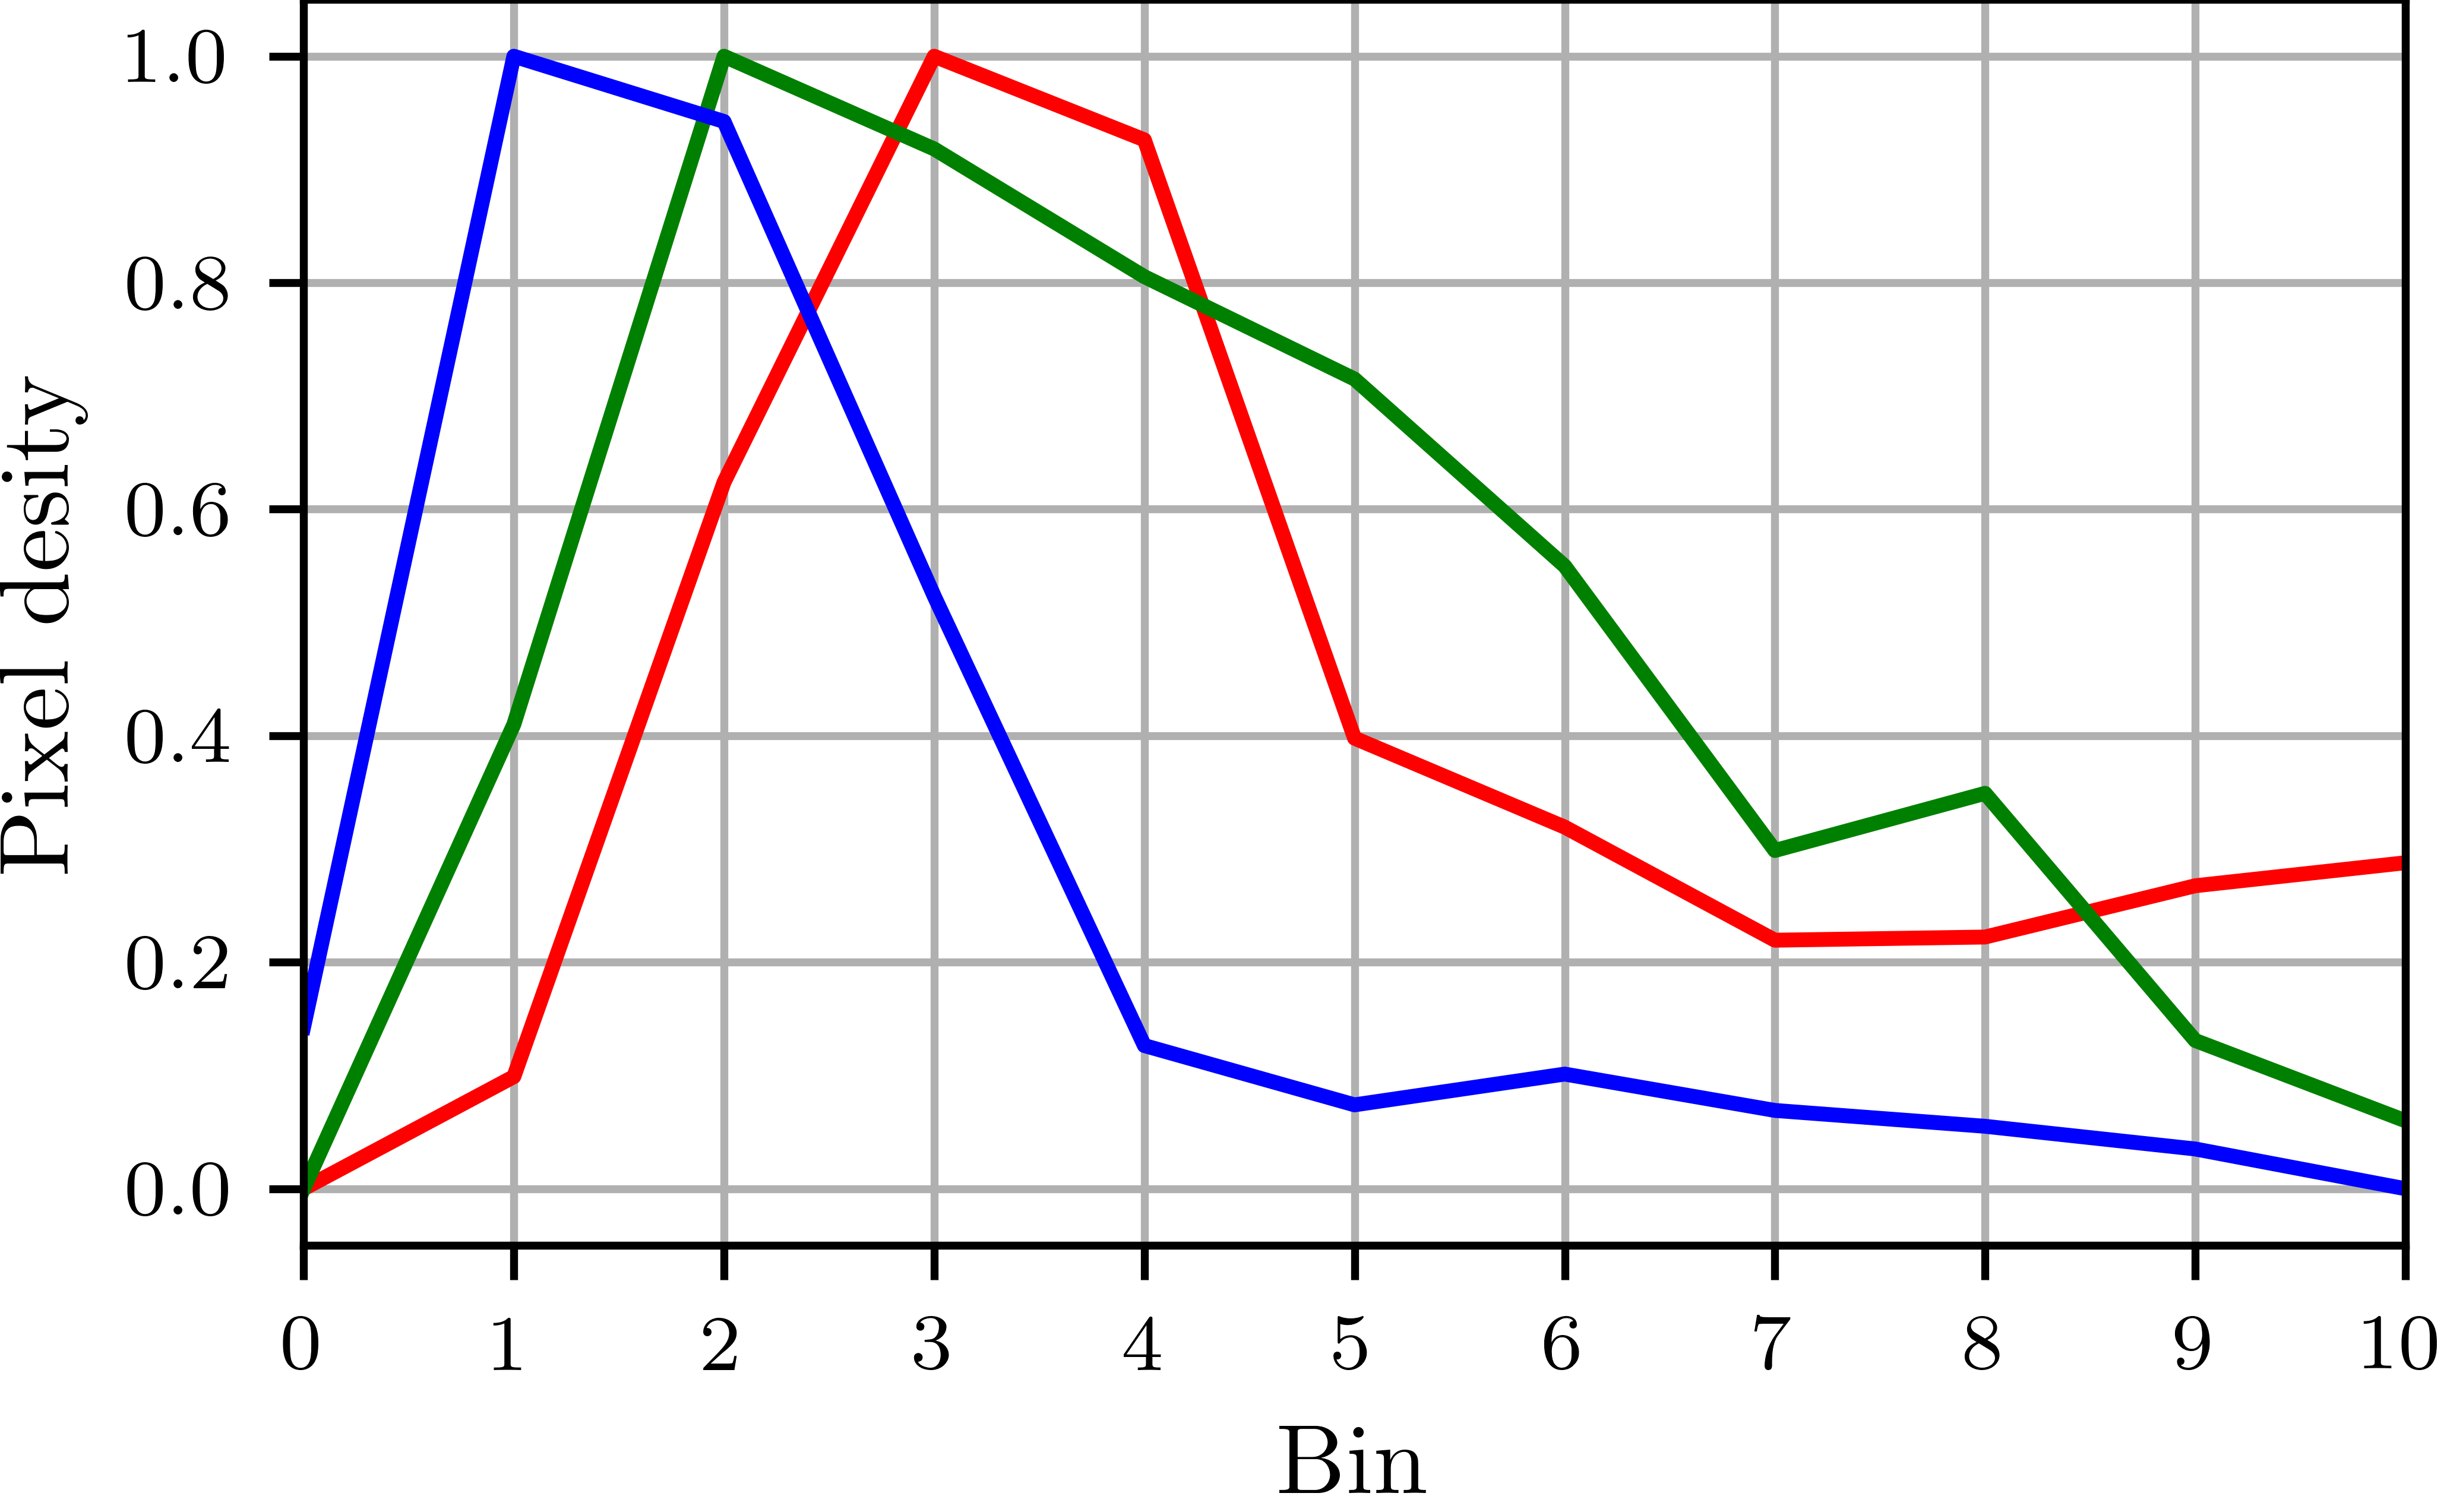
\includegraphics[width=\textwidth]{araras_single_histogram}
        \caption{Single-channel color pixel distribution}
    \end{subfigure} 
    
    \caption{}\label{fig:single_channel_histogram}    
\end{figure}
    
    
\subsubsection{3-d Color Histogram}

\begin{figure}[!ht]
    \centering
    \begin{subfigure}[b]{0.4\textwidth}
        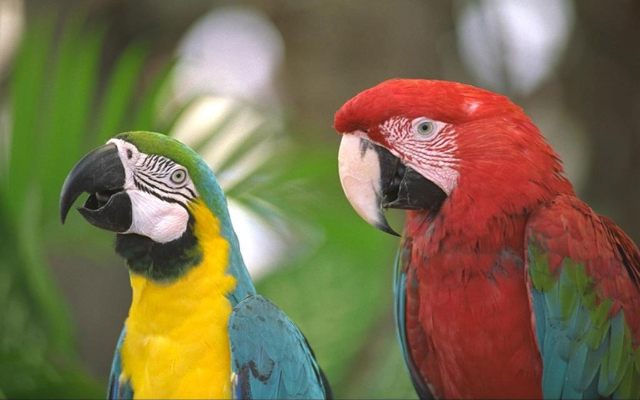
\includegraphics[width=\textwidth]{araras}
        \caption{Input image}
    \end{subfigure} \\
       
    \begin{subfigure}[b]{0.49\textwidth}
        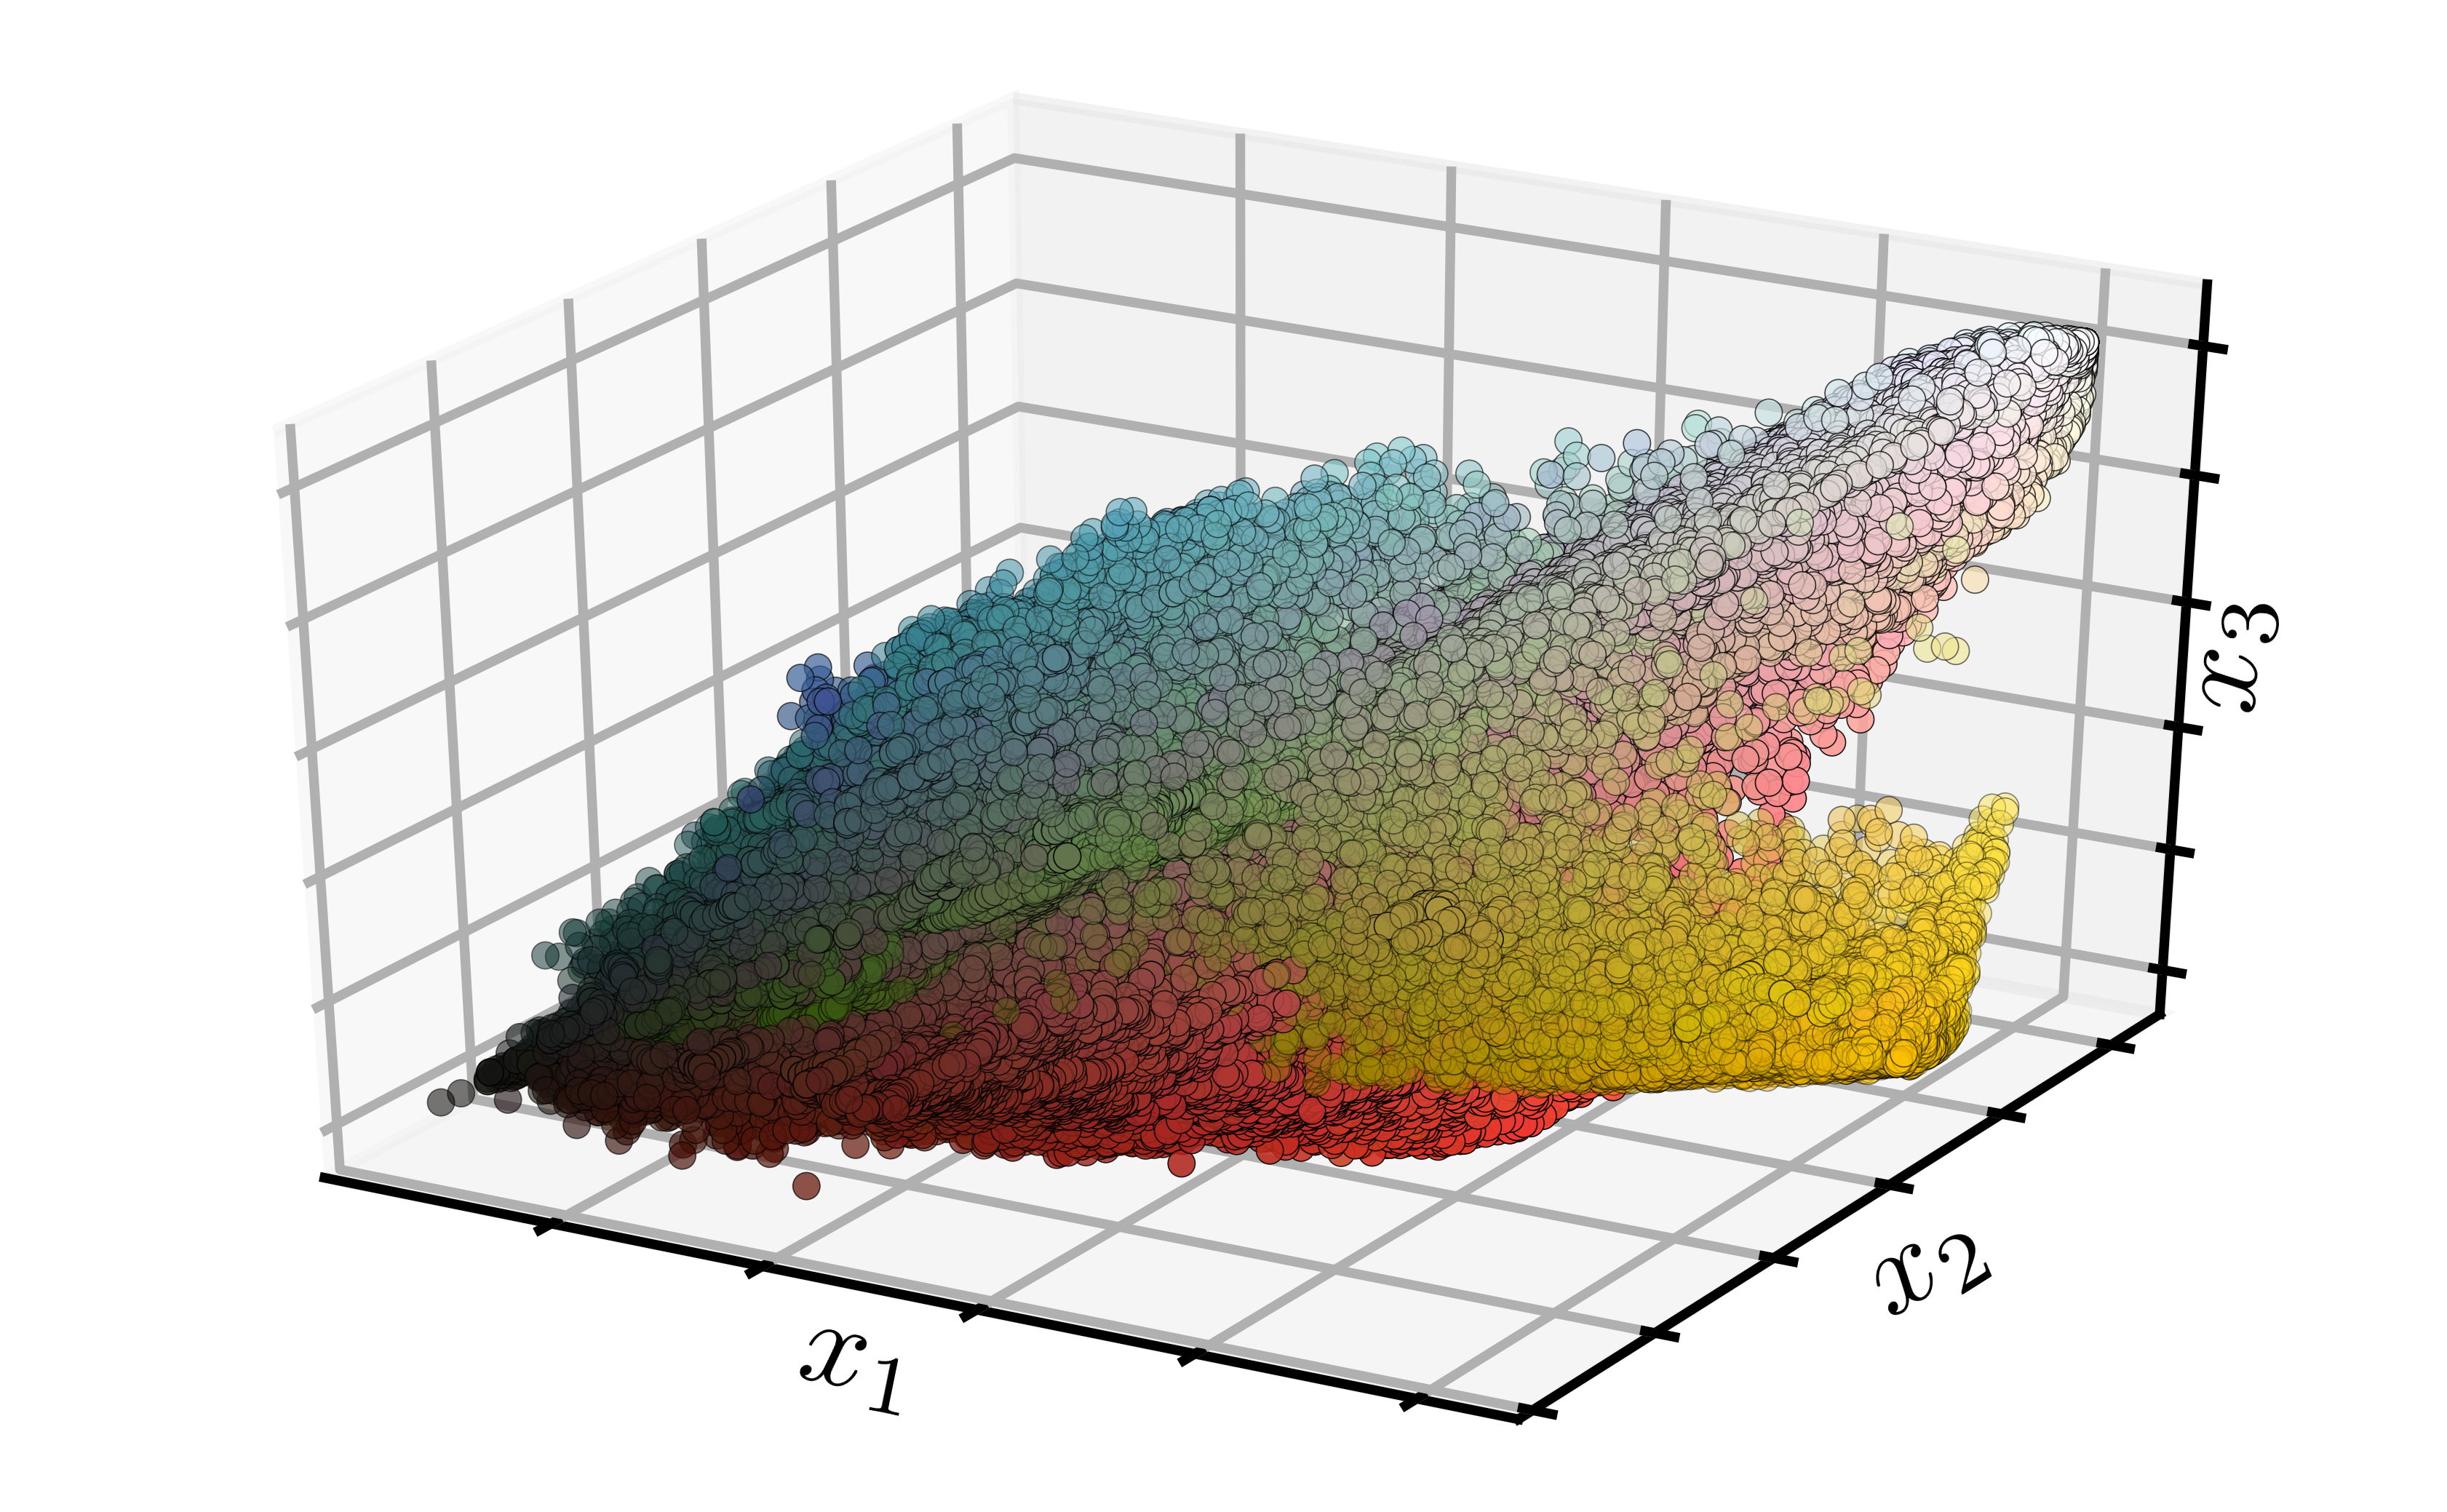
\includegraphics[width=\textwidth]{araras_3d_distribution}
        \caption{3-d image color pixel distribution}
    \end{subfigure} 
    \begin{subfigure}[b]{0.49\textwidth}
        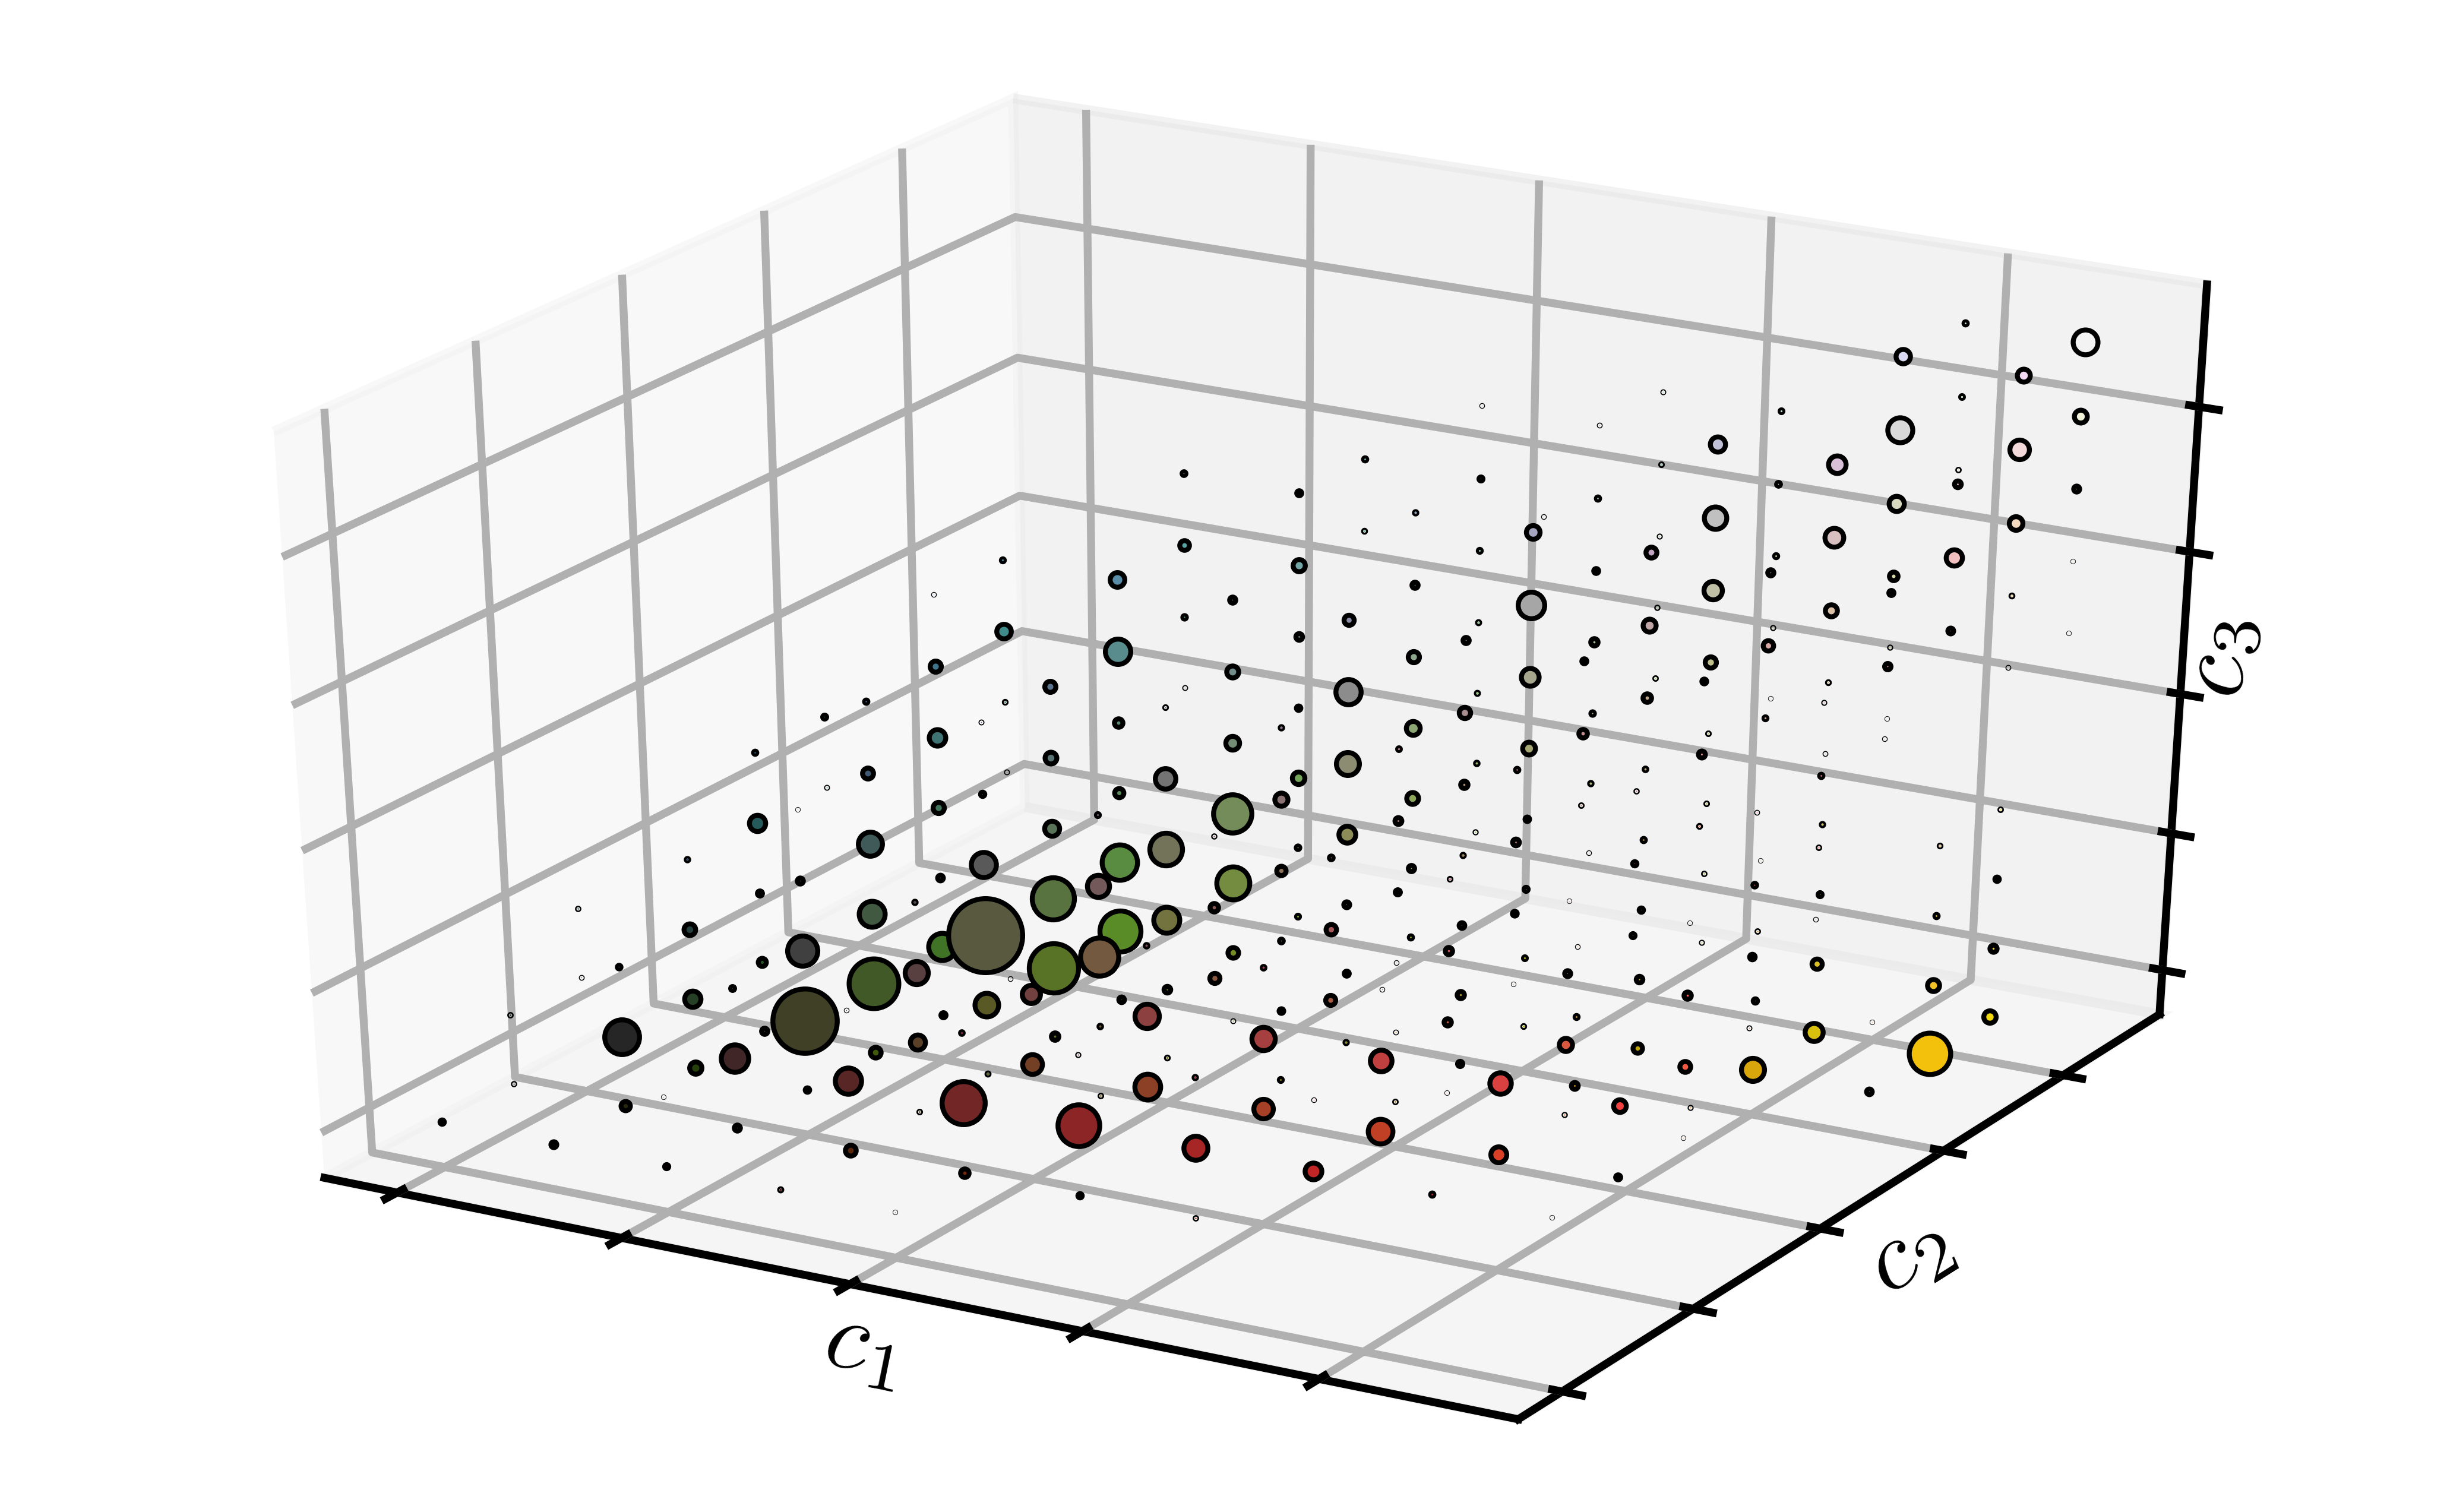
\includegraphics[width=\textwidth]{araras_3d_histogram}
        \caption{3-d color pixel histogram}
    \end{subfigure} 
    
    \caption{3-d image color representation. 3-d pixel distribution and 10 bins 3-d pixel histogram.}\label{fig:3d_color_representation}    
\end{figure}


\subsubsection{Color Signature}

\begin{figure}[!ht]
    \centering
    \begin{subfigure}[b]{0.4\textwidth}
        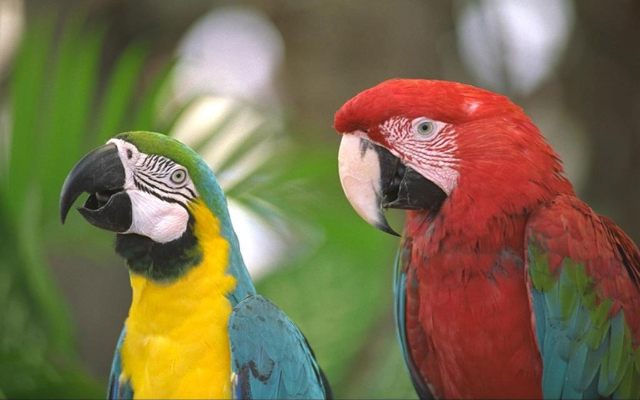
\includegraphics[width=\textwidth]{araras}
        \caption{Input image}
    \end{subfigure} \\
    
    \begin{subfigure}[b]{0.4\textwidth}
    	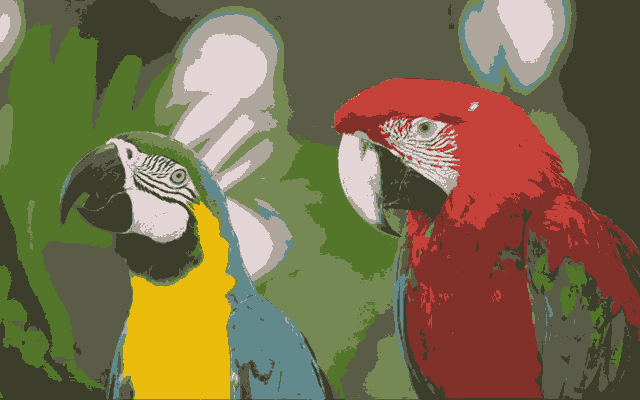
\includegraphics[width=\textwidth]{araras_color_clusters}
        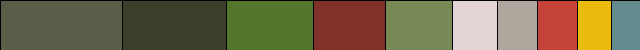
\includegraphics[width=\textwidth]{araras_bar_signature}
        \caption{Color signature}
    \end{subfigure}
    	~ %add desired spacing between images, e. g. ~, \quad, \qquad, \hfill etc. 
      %(or a blank line to force the subfigure onto a new line)
    \begin{subfigure}[b]{0.5\textwidth}
        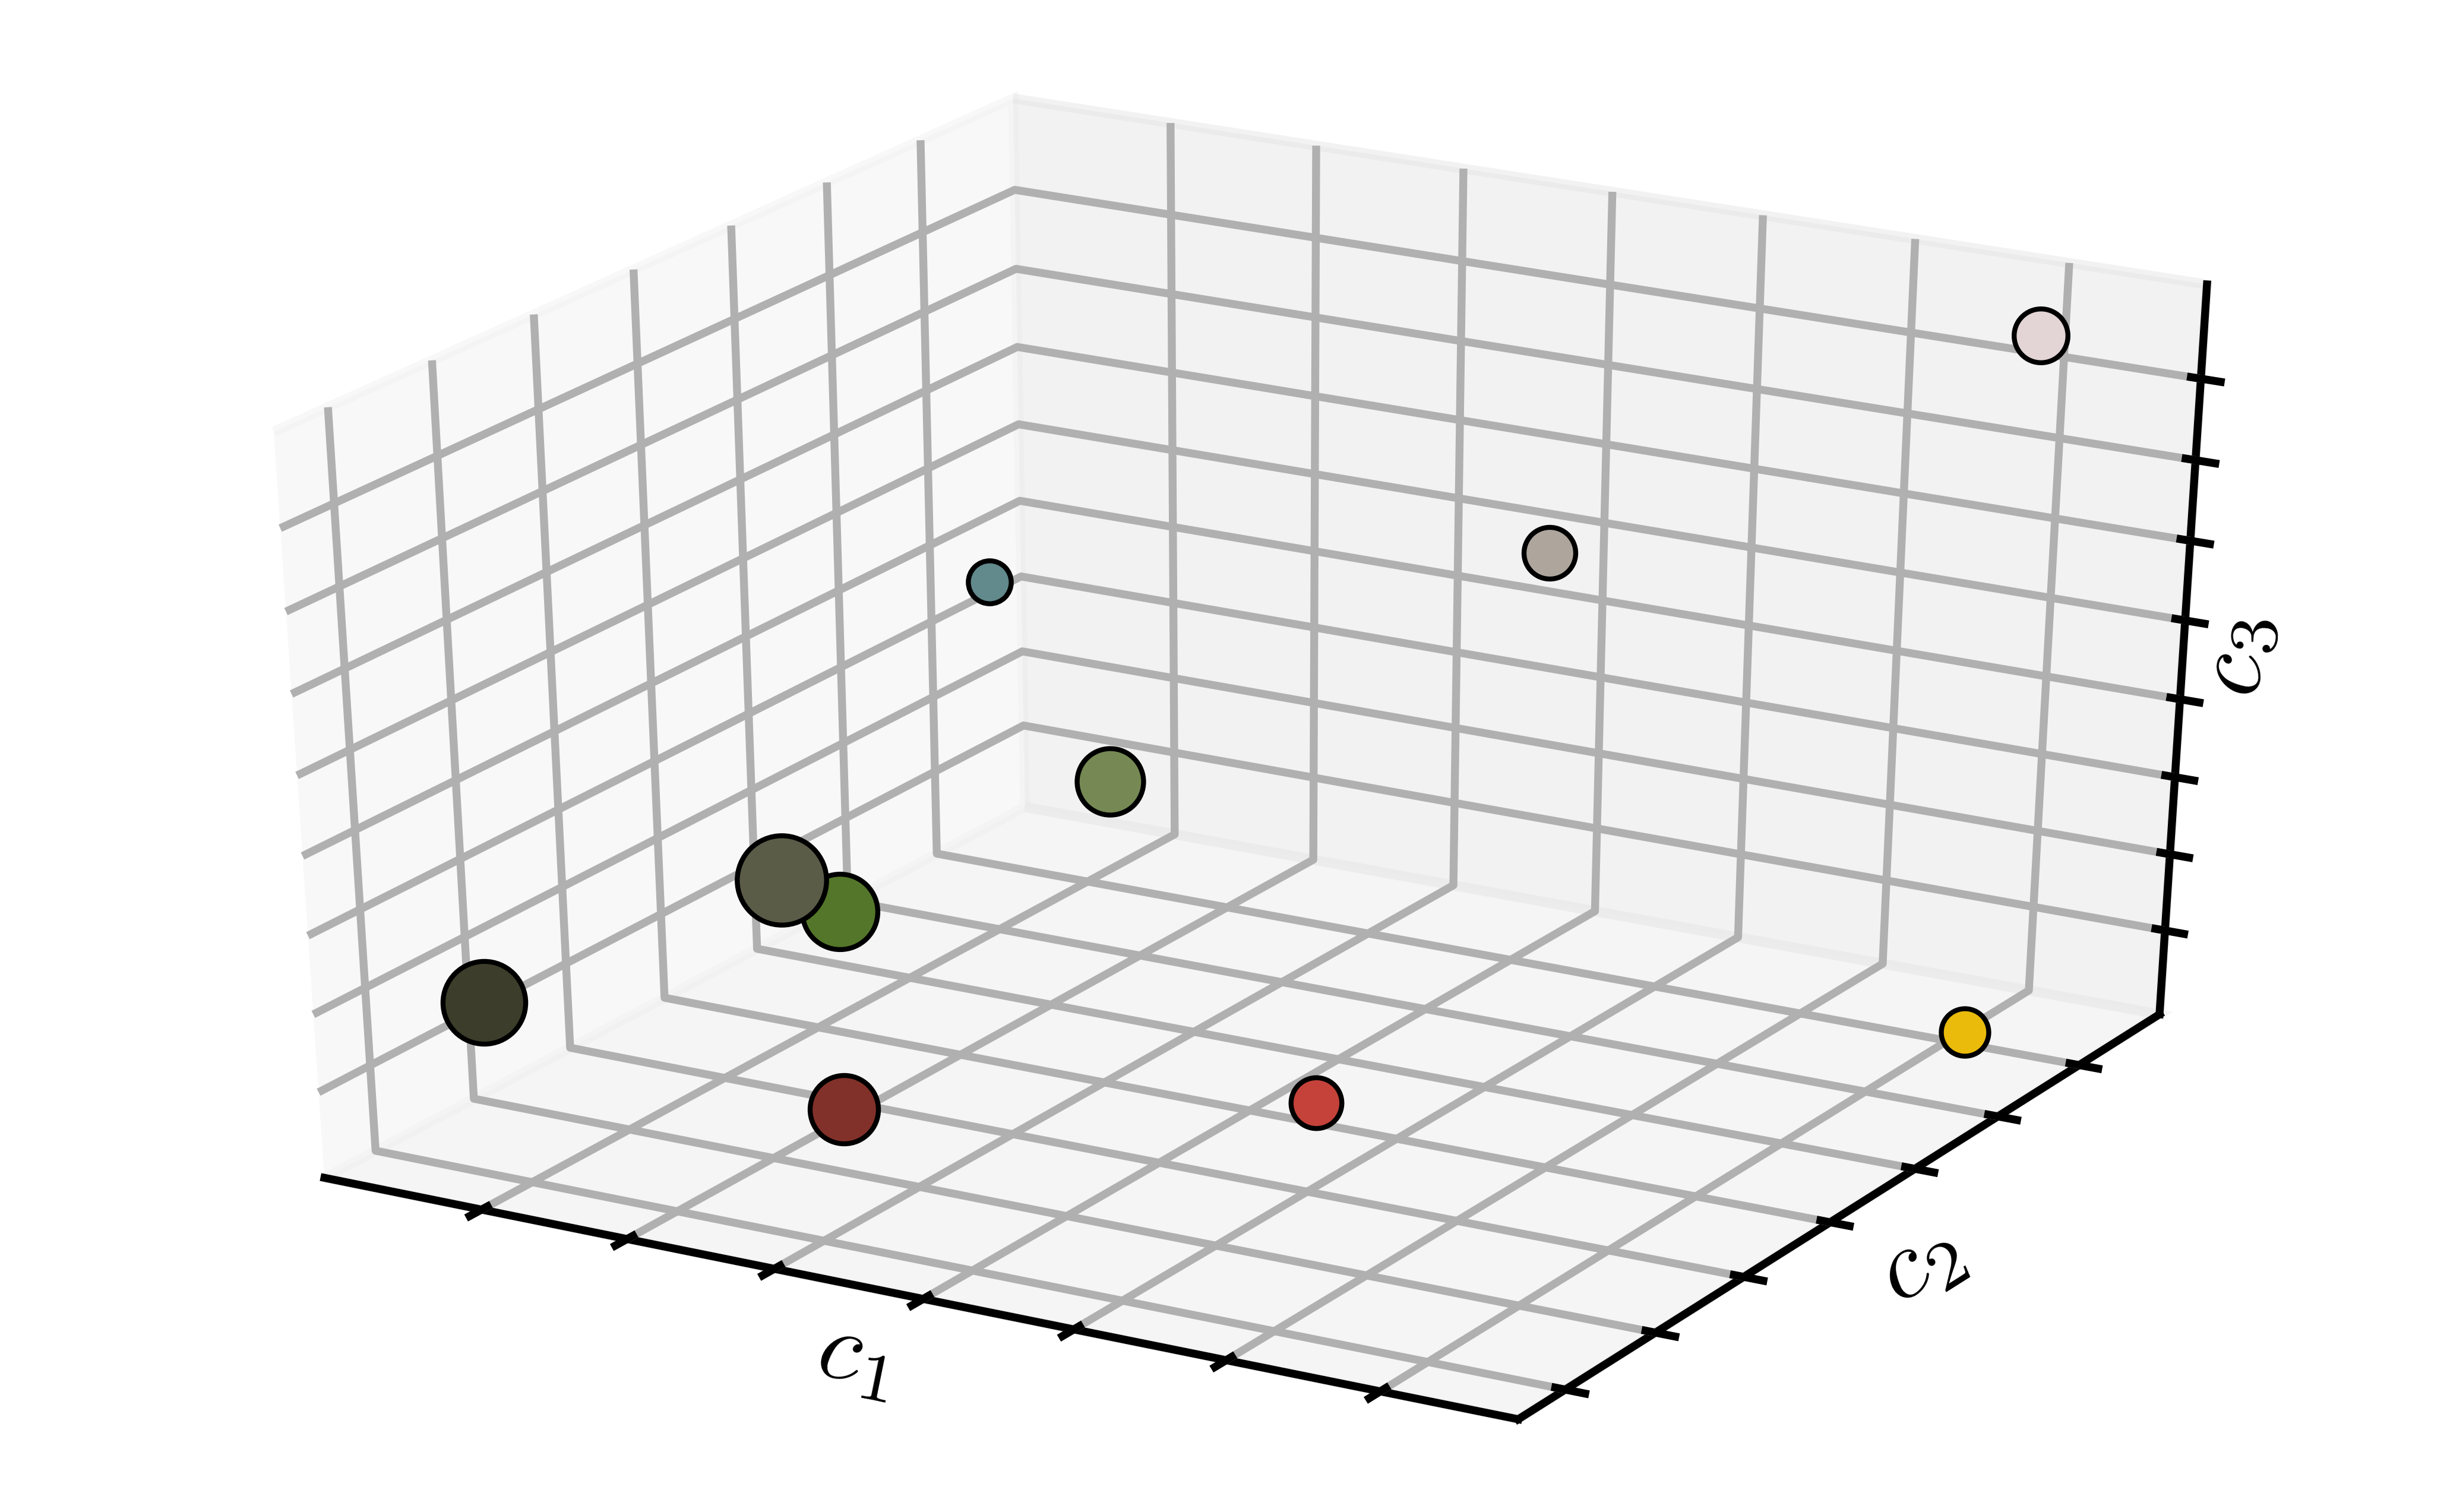
\includegraphics[width=\textwidth]{araras_3d_signature}
        \caption{3-d representation of color ignature}
    \end{subfigure} 
    	    
    \caption{Image color signature and the 3-d visualization of signature clusters.}\label{fig:color_signature}    
\end{figure}



\begin{figure}[!ht]
    \centering
    \begin{subfigure}[t]{\dimexpr0.32\textwidth+20pt\relax}
    	\makebox[20pt]{\raisebox{40pt}{ \small\textbf{\textsf{(a)}} }}%
    	
\includegraphics[width=\dimexpr\linewidth-20pt\relax]{tempo}
    \end{subfigure}~ 
%    \begin{subfigure}[b]{0.32\textwidth}
%        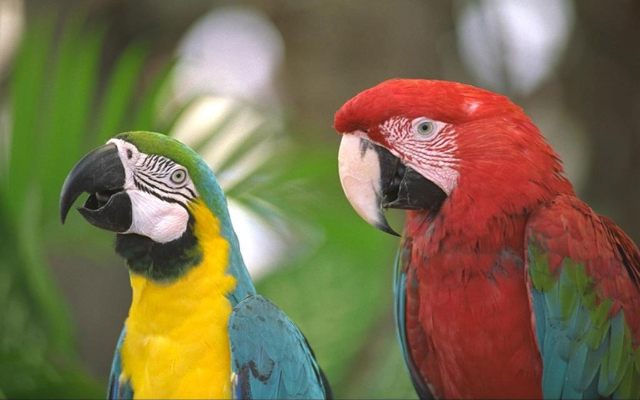
\includegraphics[width=\textwidth]{araras}
%    \end{subfigure}~
    \begin{subfigure}[b]{0.32\textwidth}
        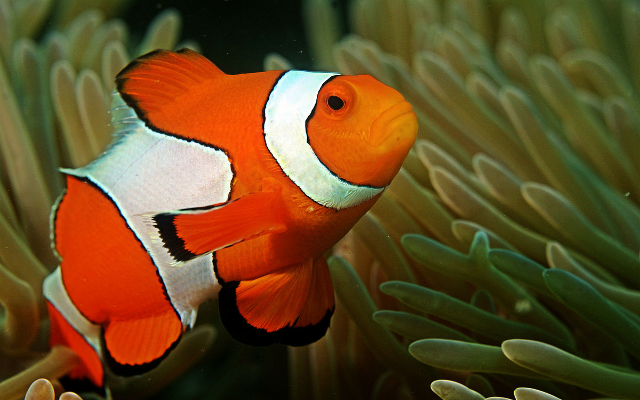
\includegraphics[width=\textwidth]{clownfish}
    \end{subfigure}~
    \begin{subfigure}[b]{0.32\textwidth}
        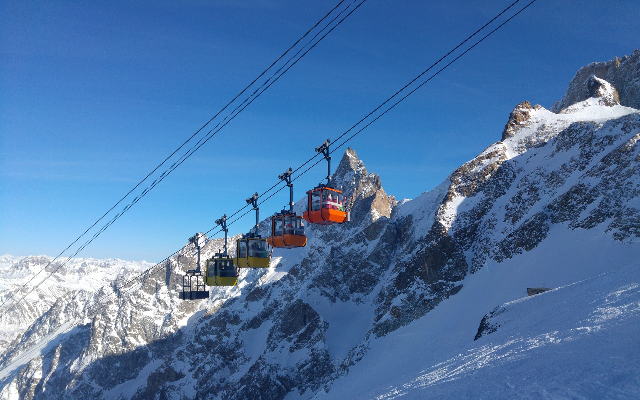
\includegraphics[width=\textwidth]{mountain}
    \end{subfigure}\vspace{10pt}
    
    \begin{subfigure}[t]{\dimexpr0.32\textwidth+20pt\relax}
    	\makebox[20pt]{\raisebox{40pt}{ \small\textbf{\textsf{(b)}} }}%
    	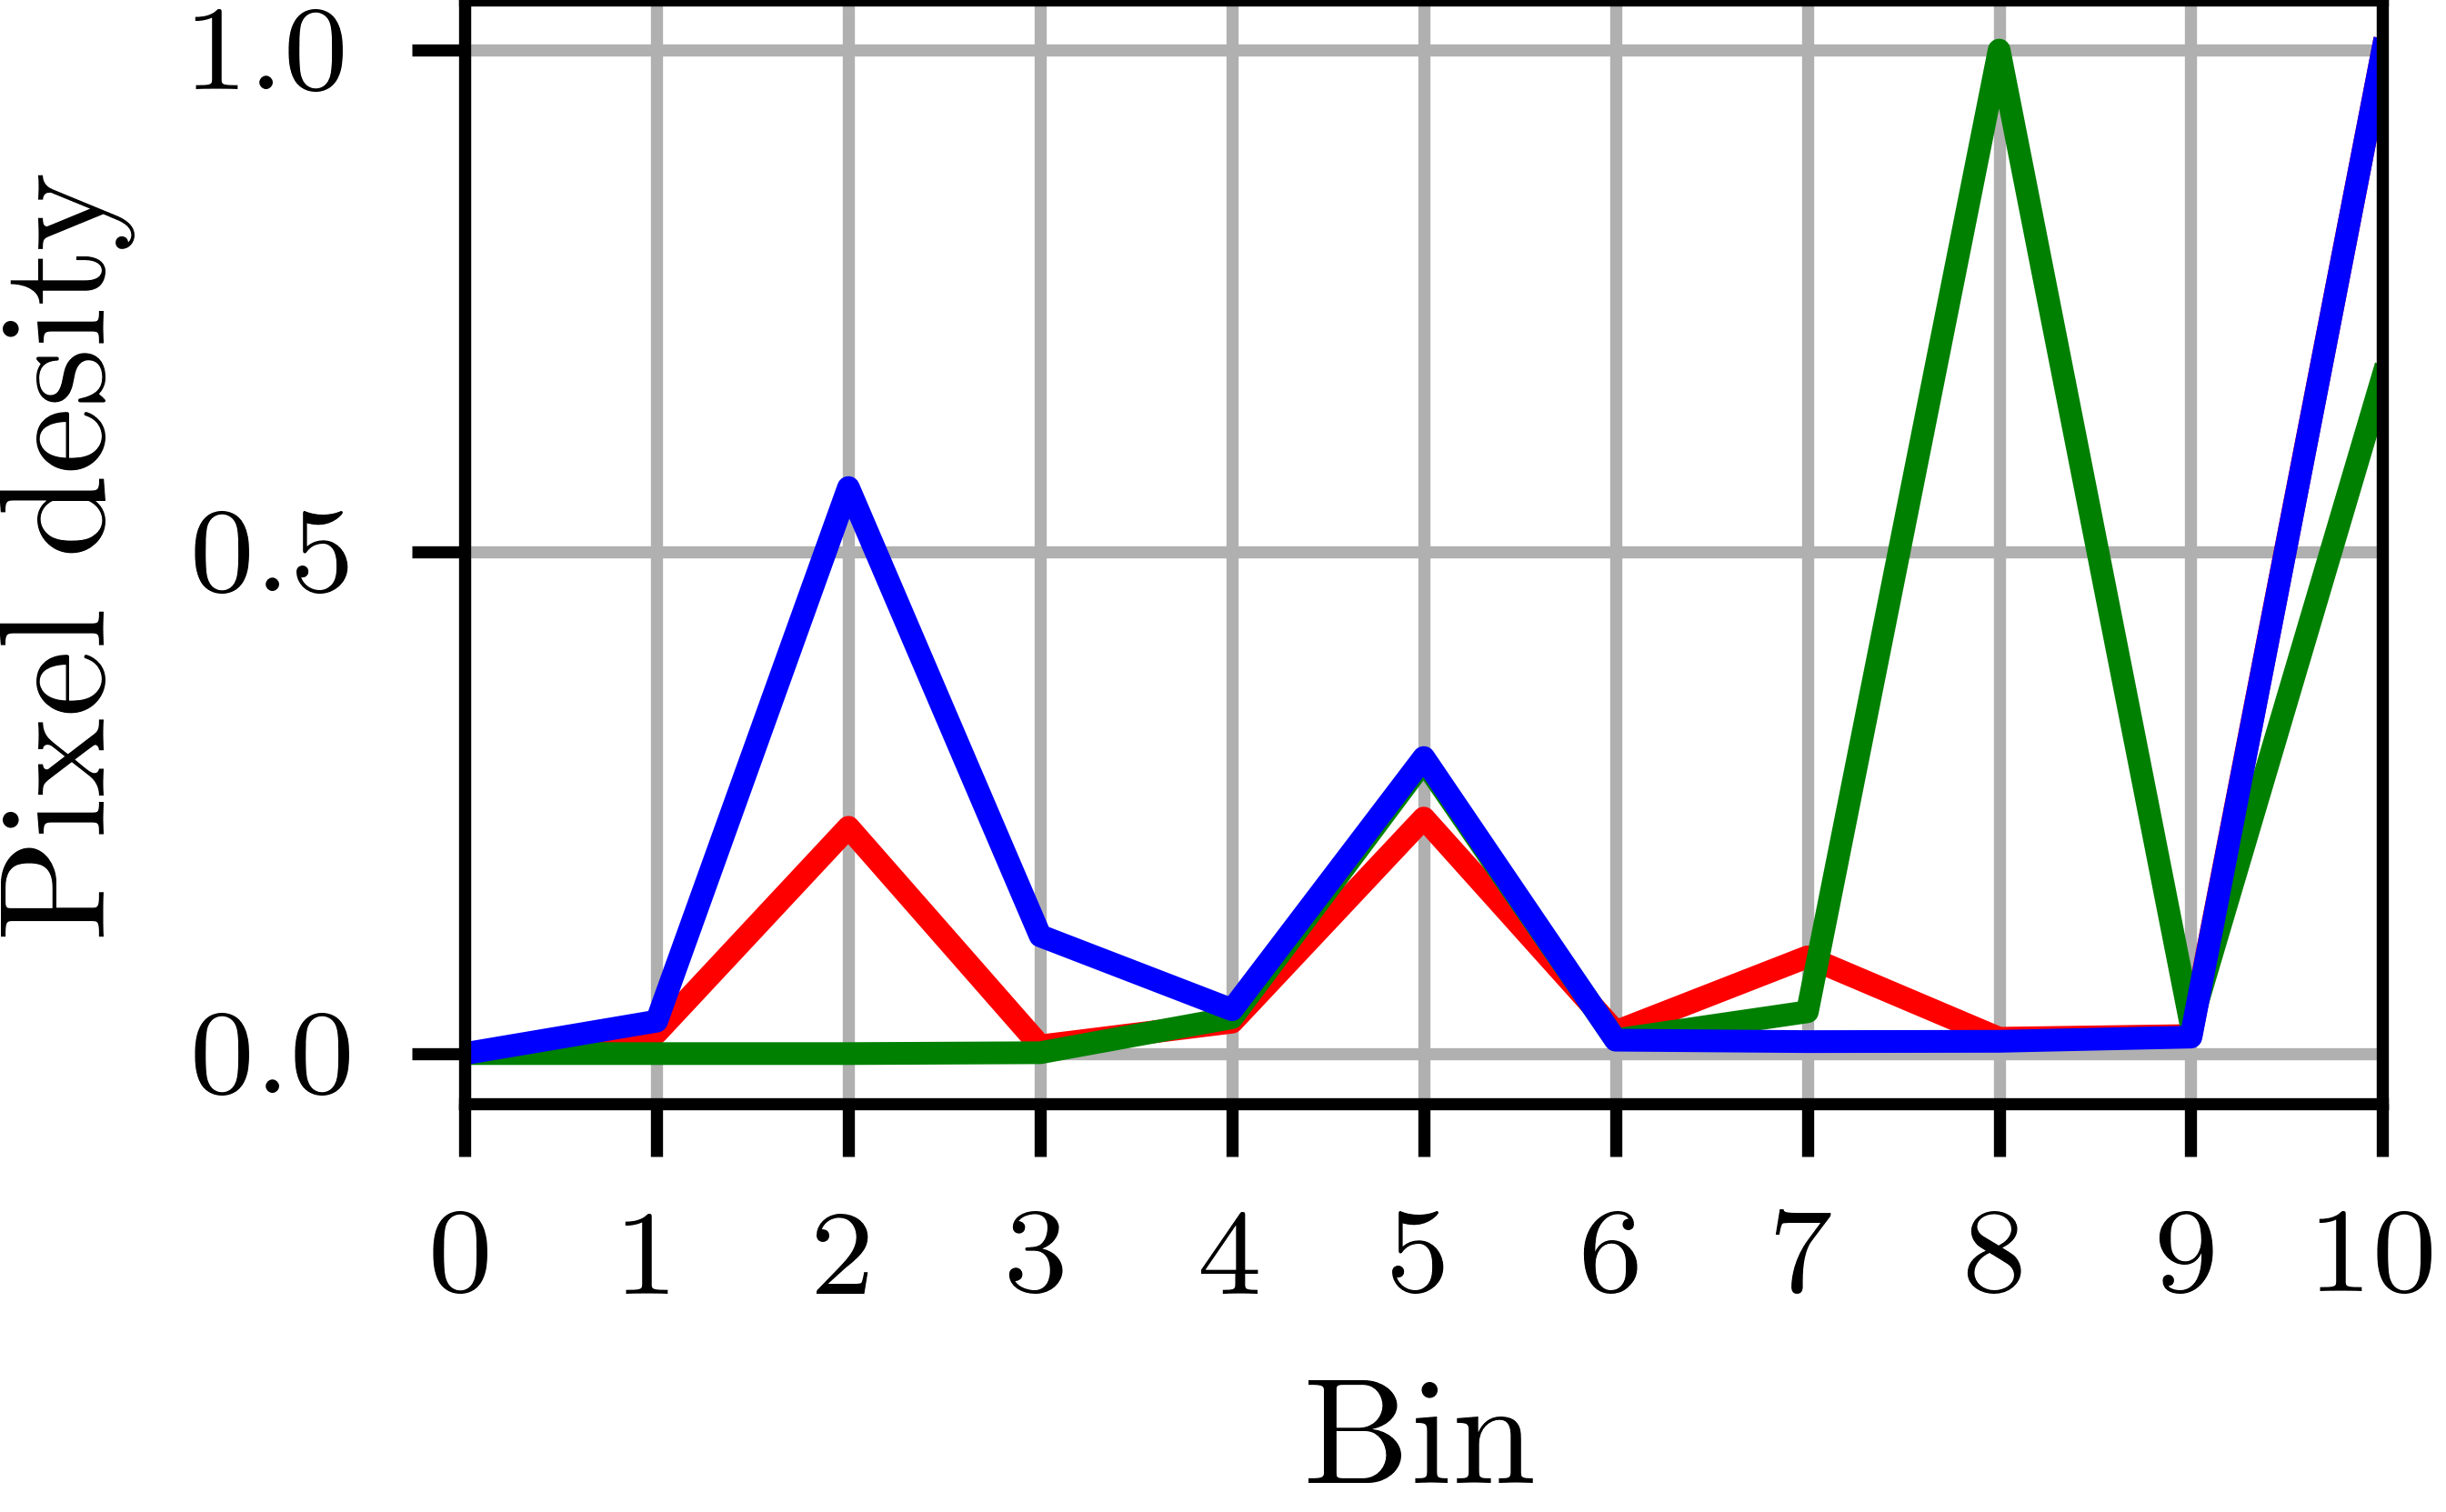
\includegraphics[width=\dimexpr\linewidth-20pt\relax]{tempo_single_histogram}
    \end{subfigure}~     
%    \begin{subfigure}[b]{0.32\textwidth}
%        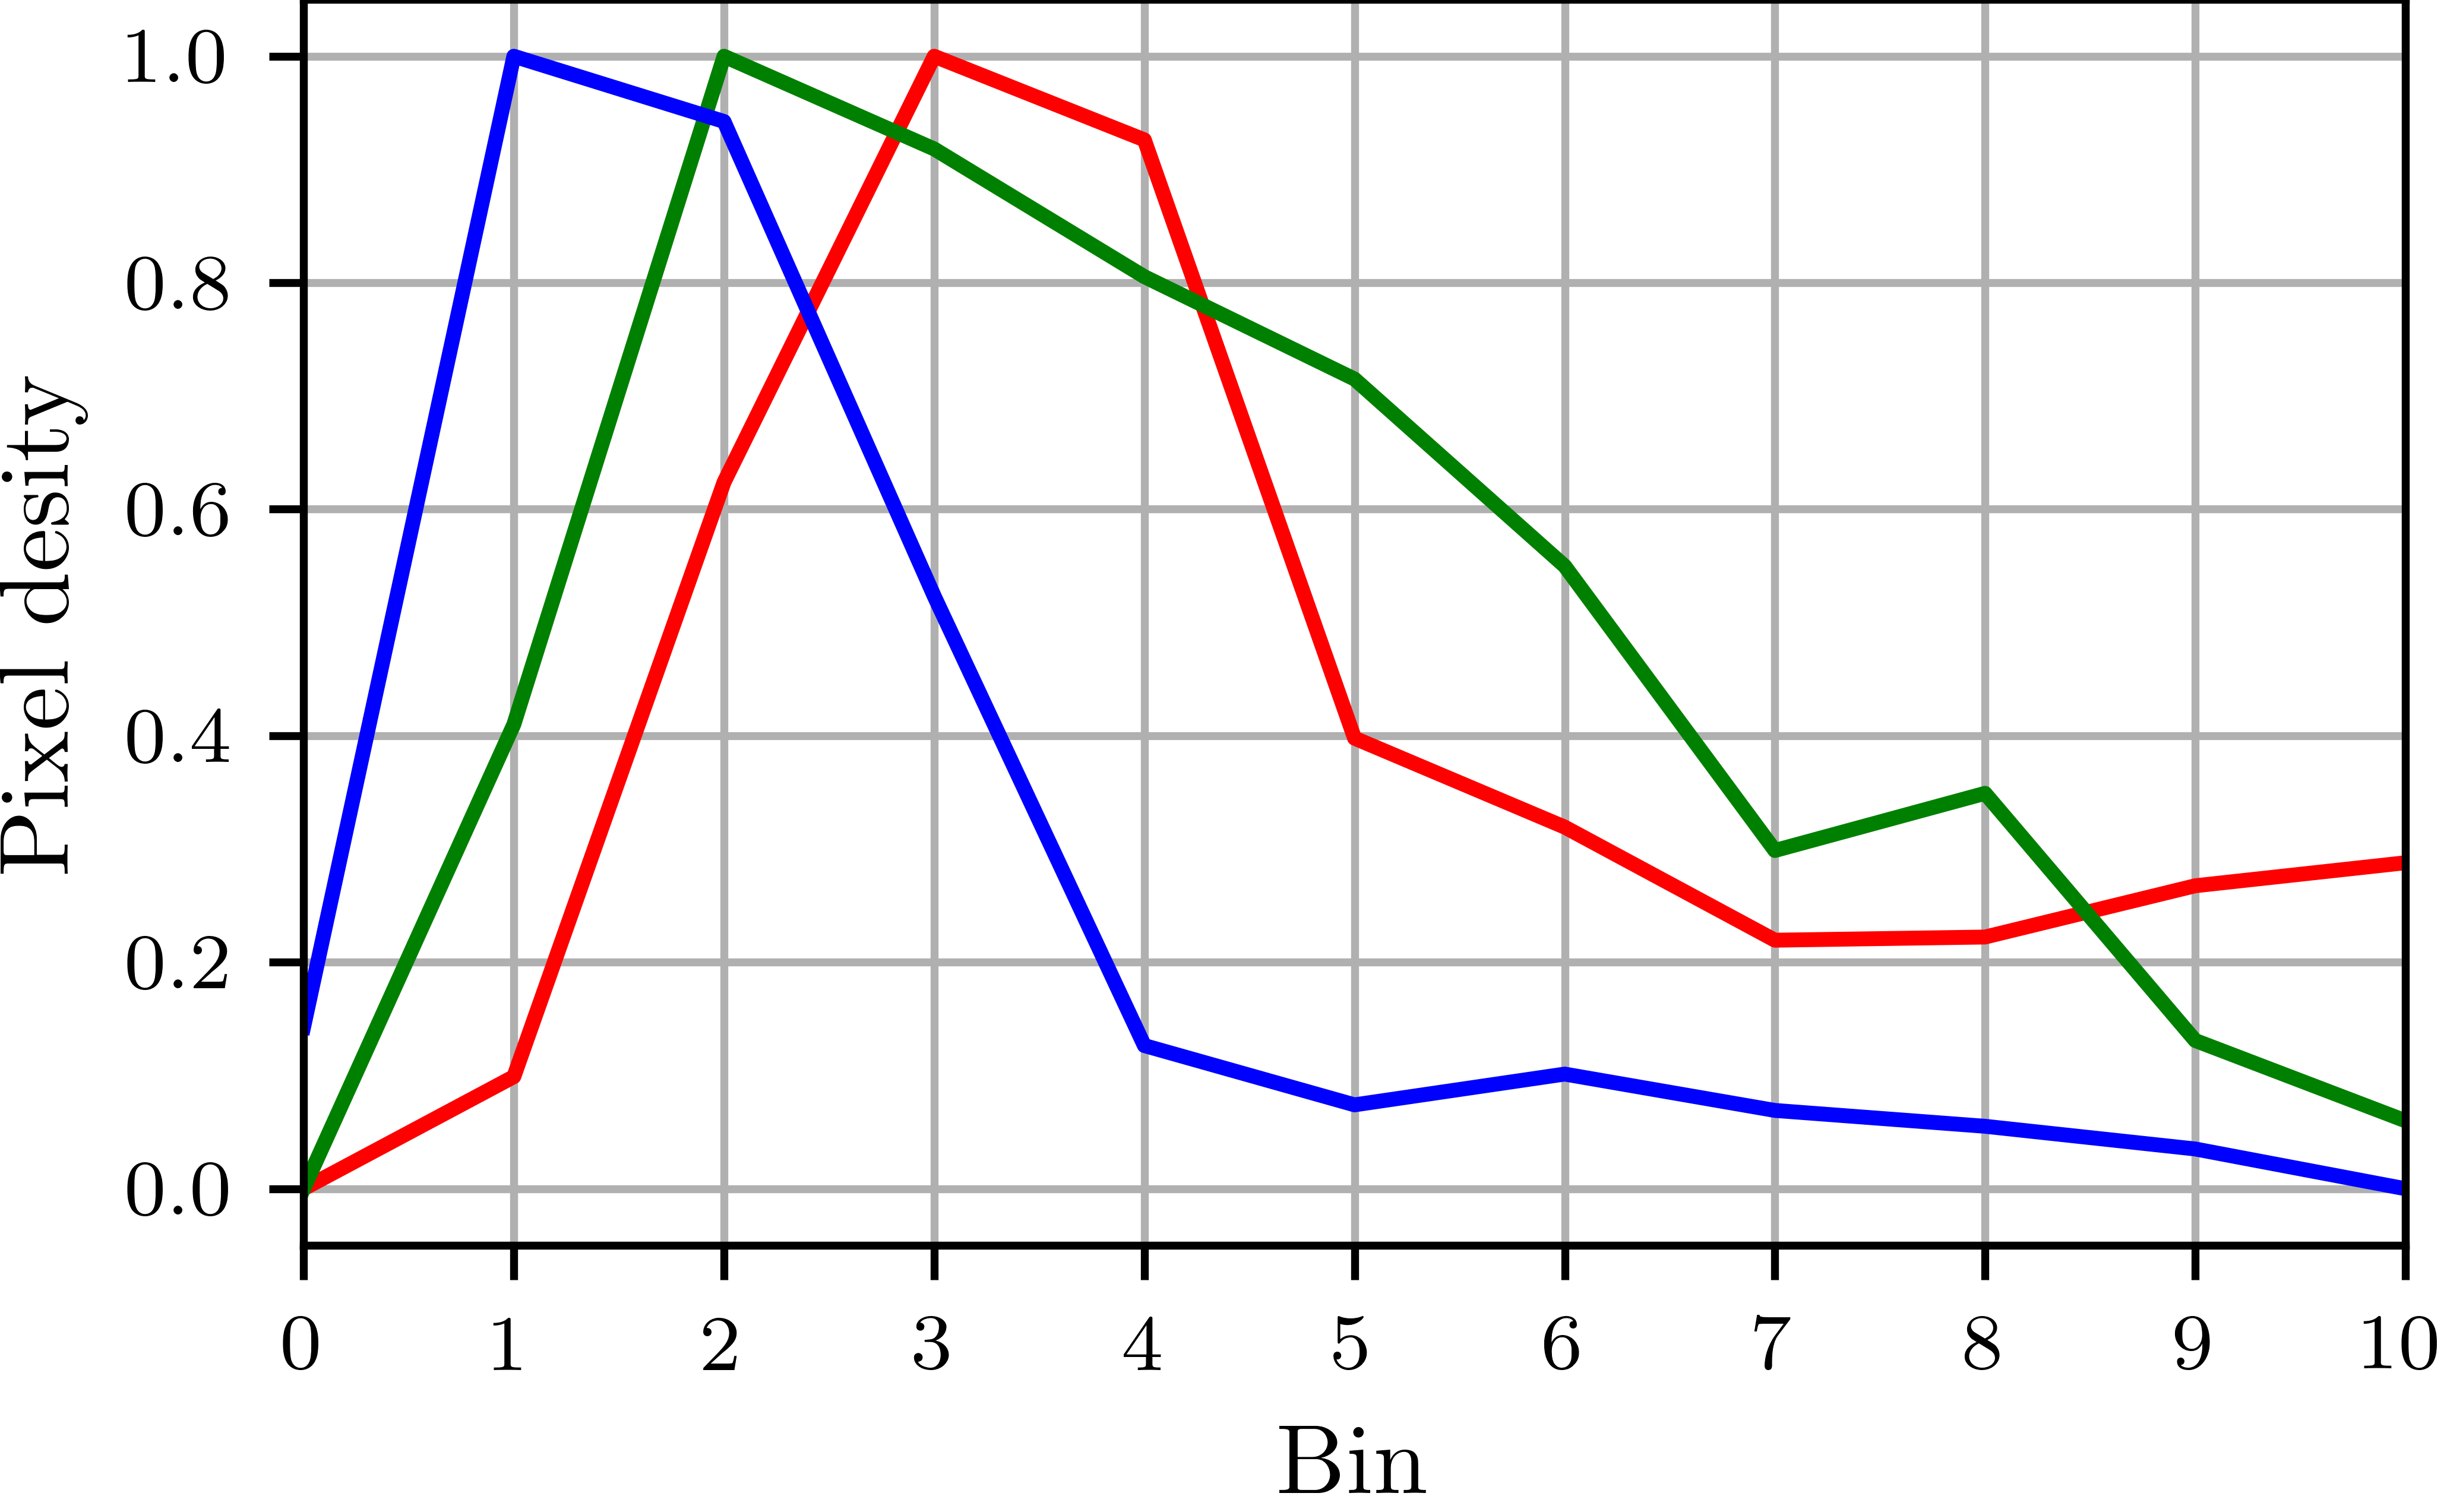
\includegraphics[width=\textwidth]{araras_single_histogram}
%    \end{subfigure}~
    \begin{subfigure}[b]{0.32\textwidth}
        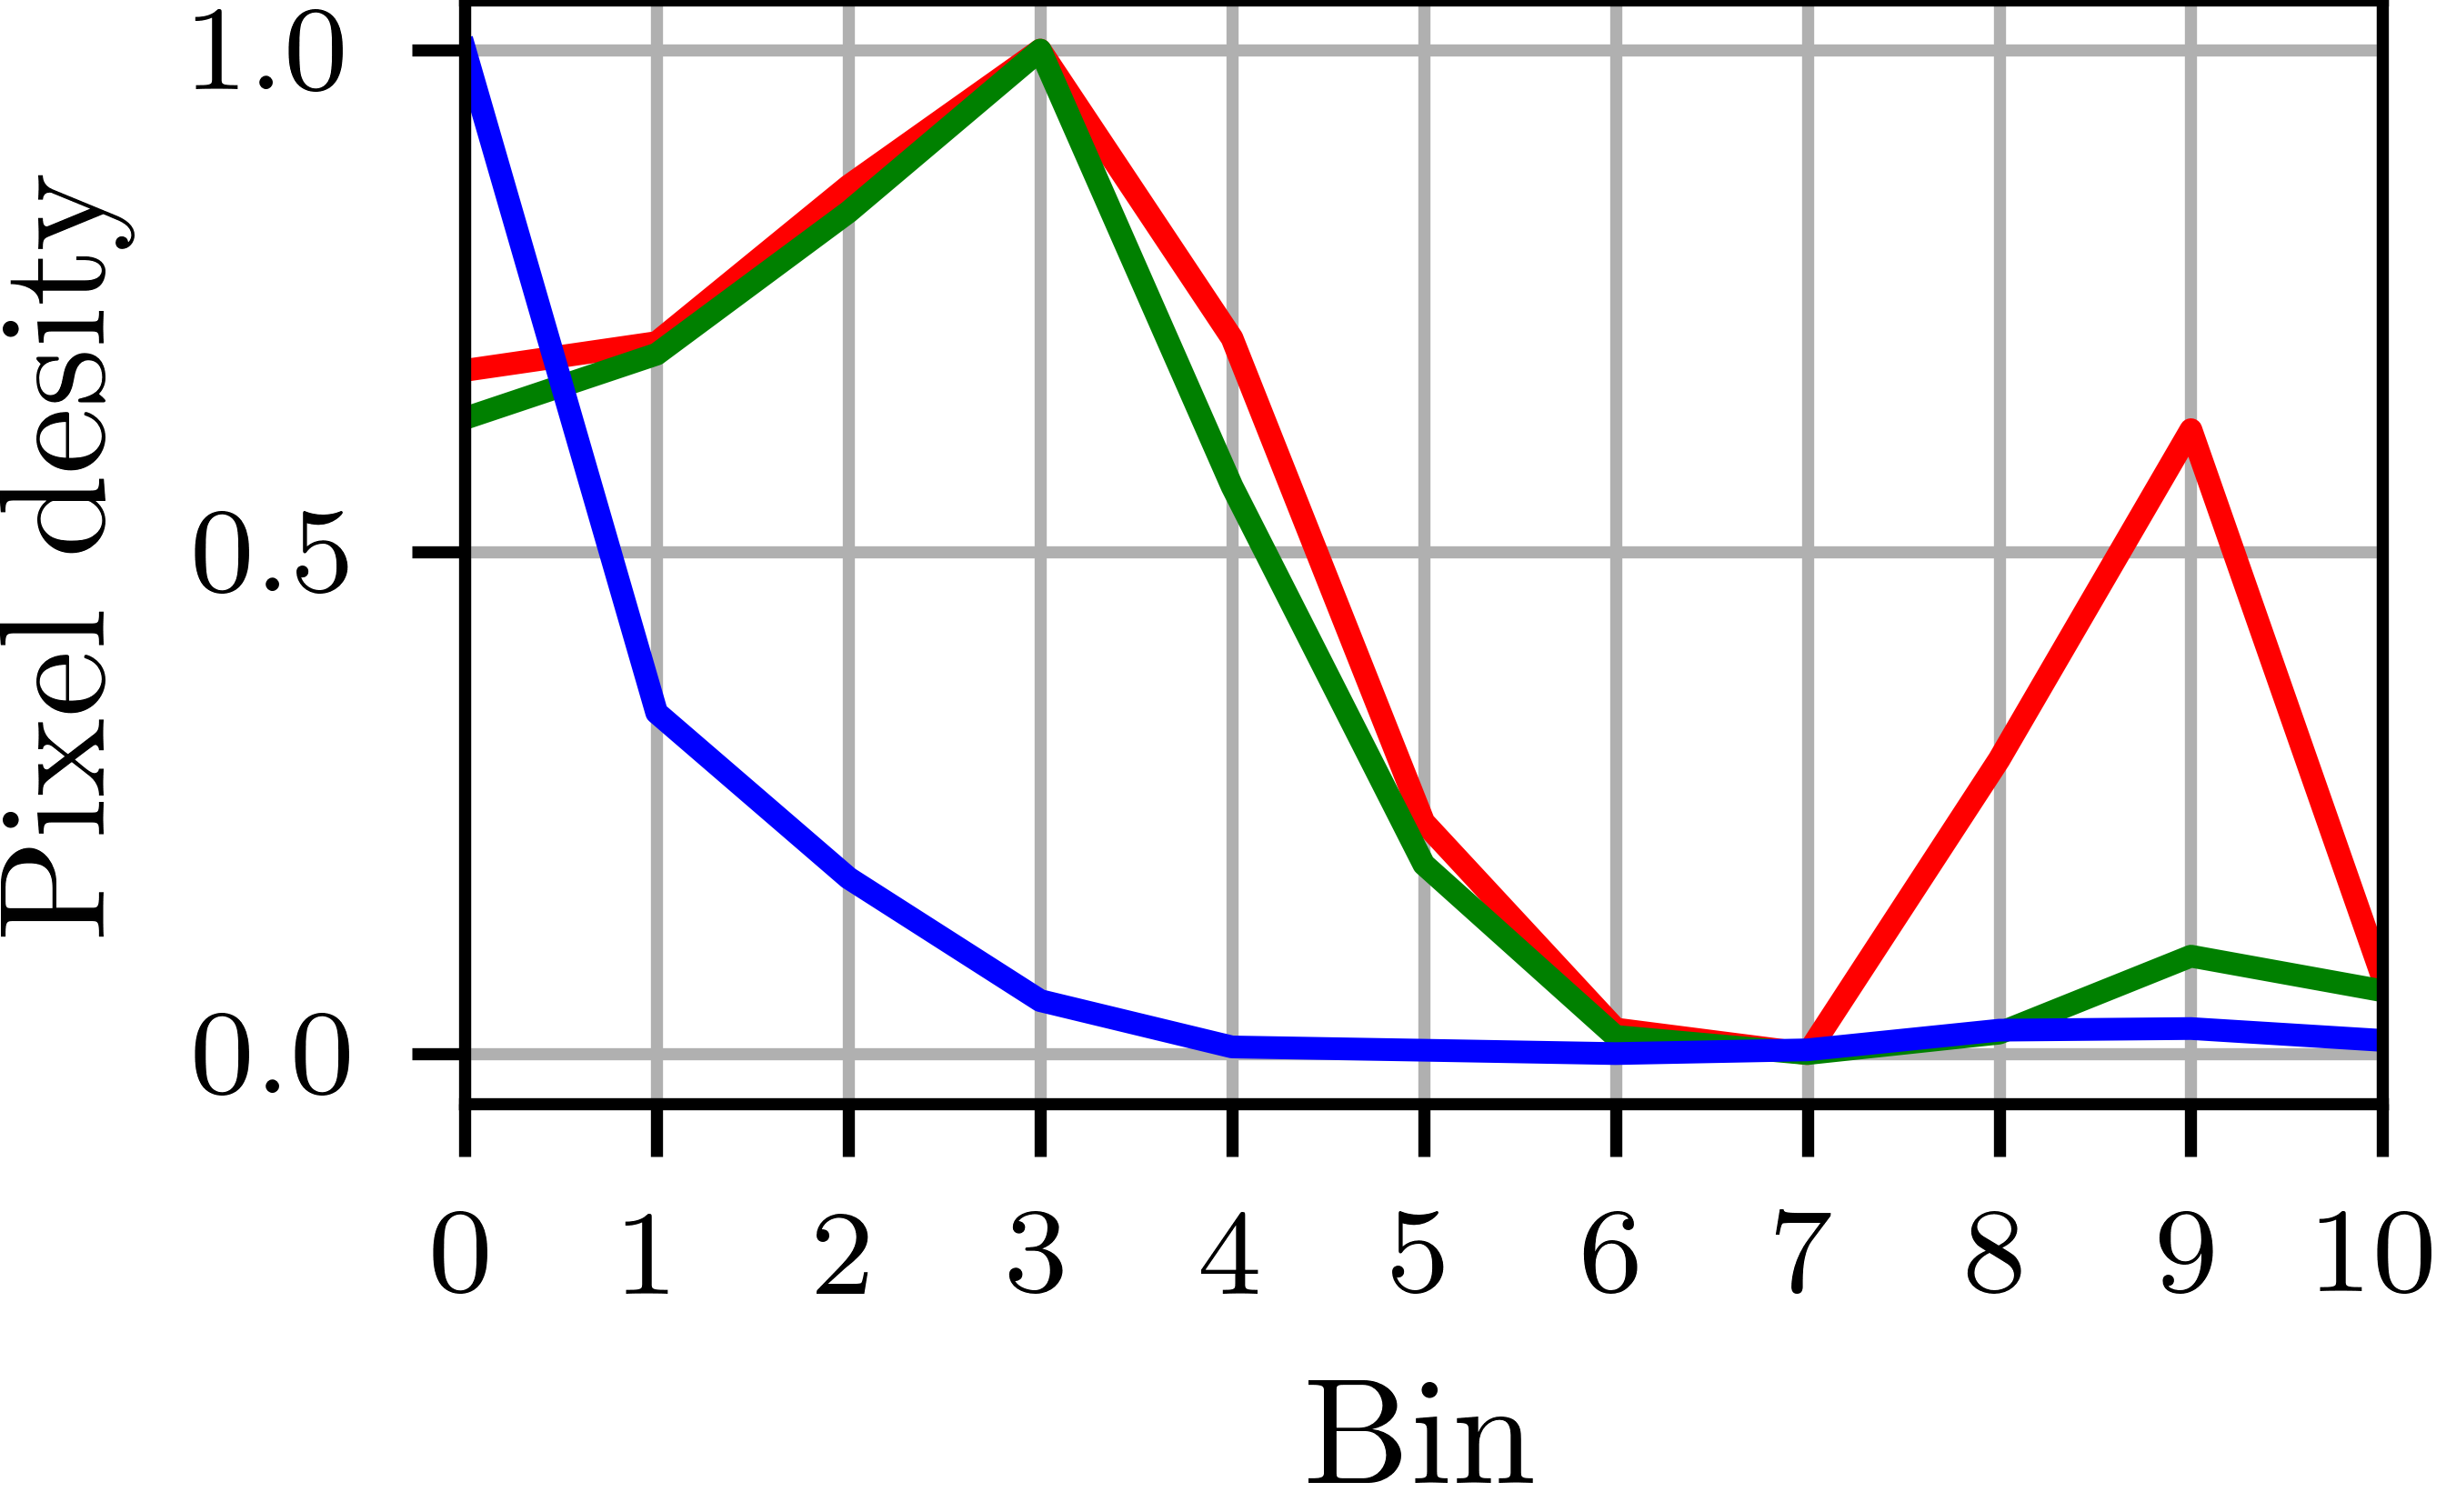
\includegraphics[width=\textwidth]{clownfish_single_histogram}
    \end{subfigure}~
    \begin{subfigure}[b]{0.32\textwidth}
        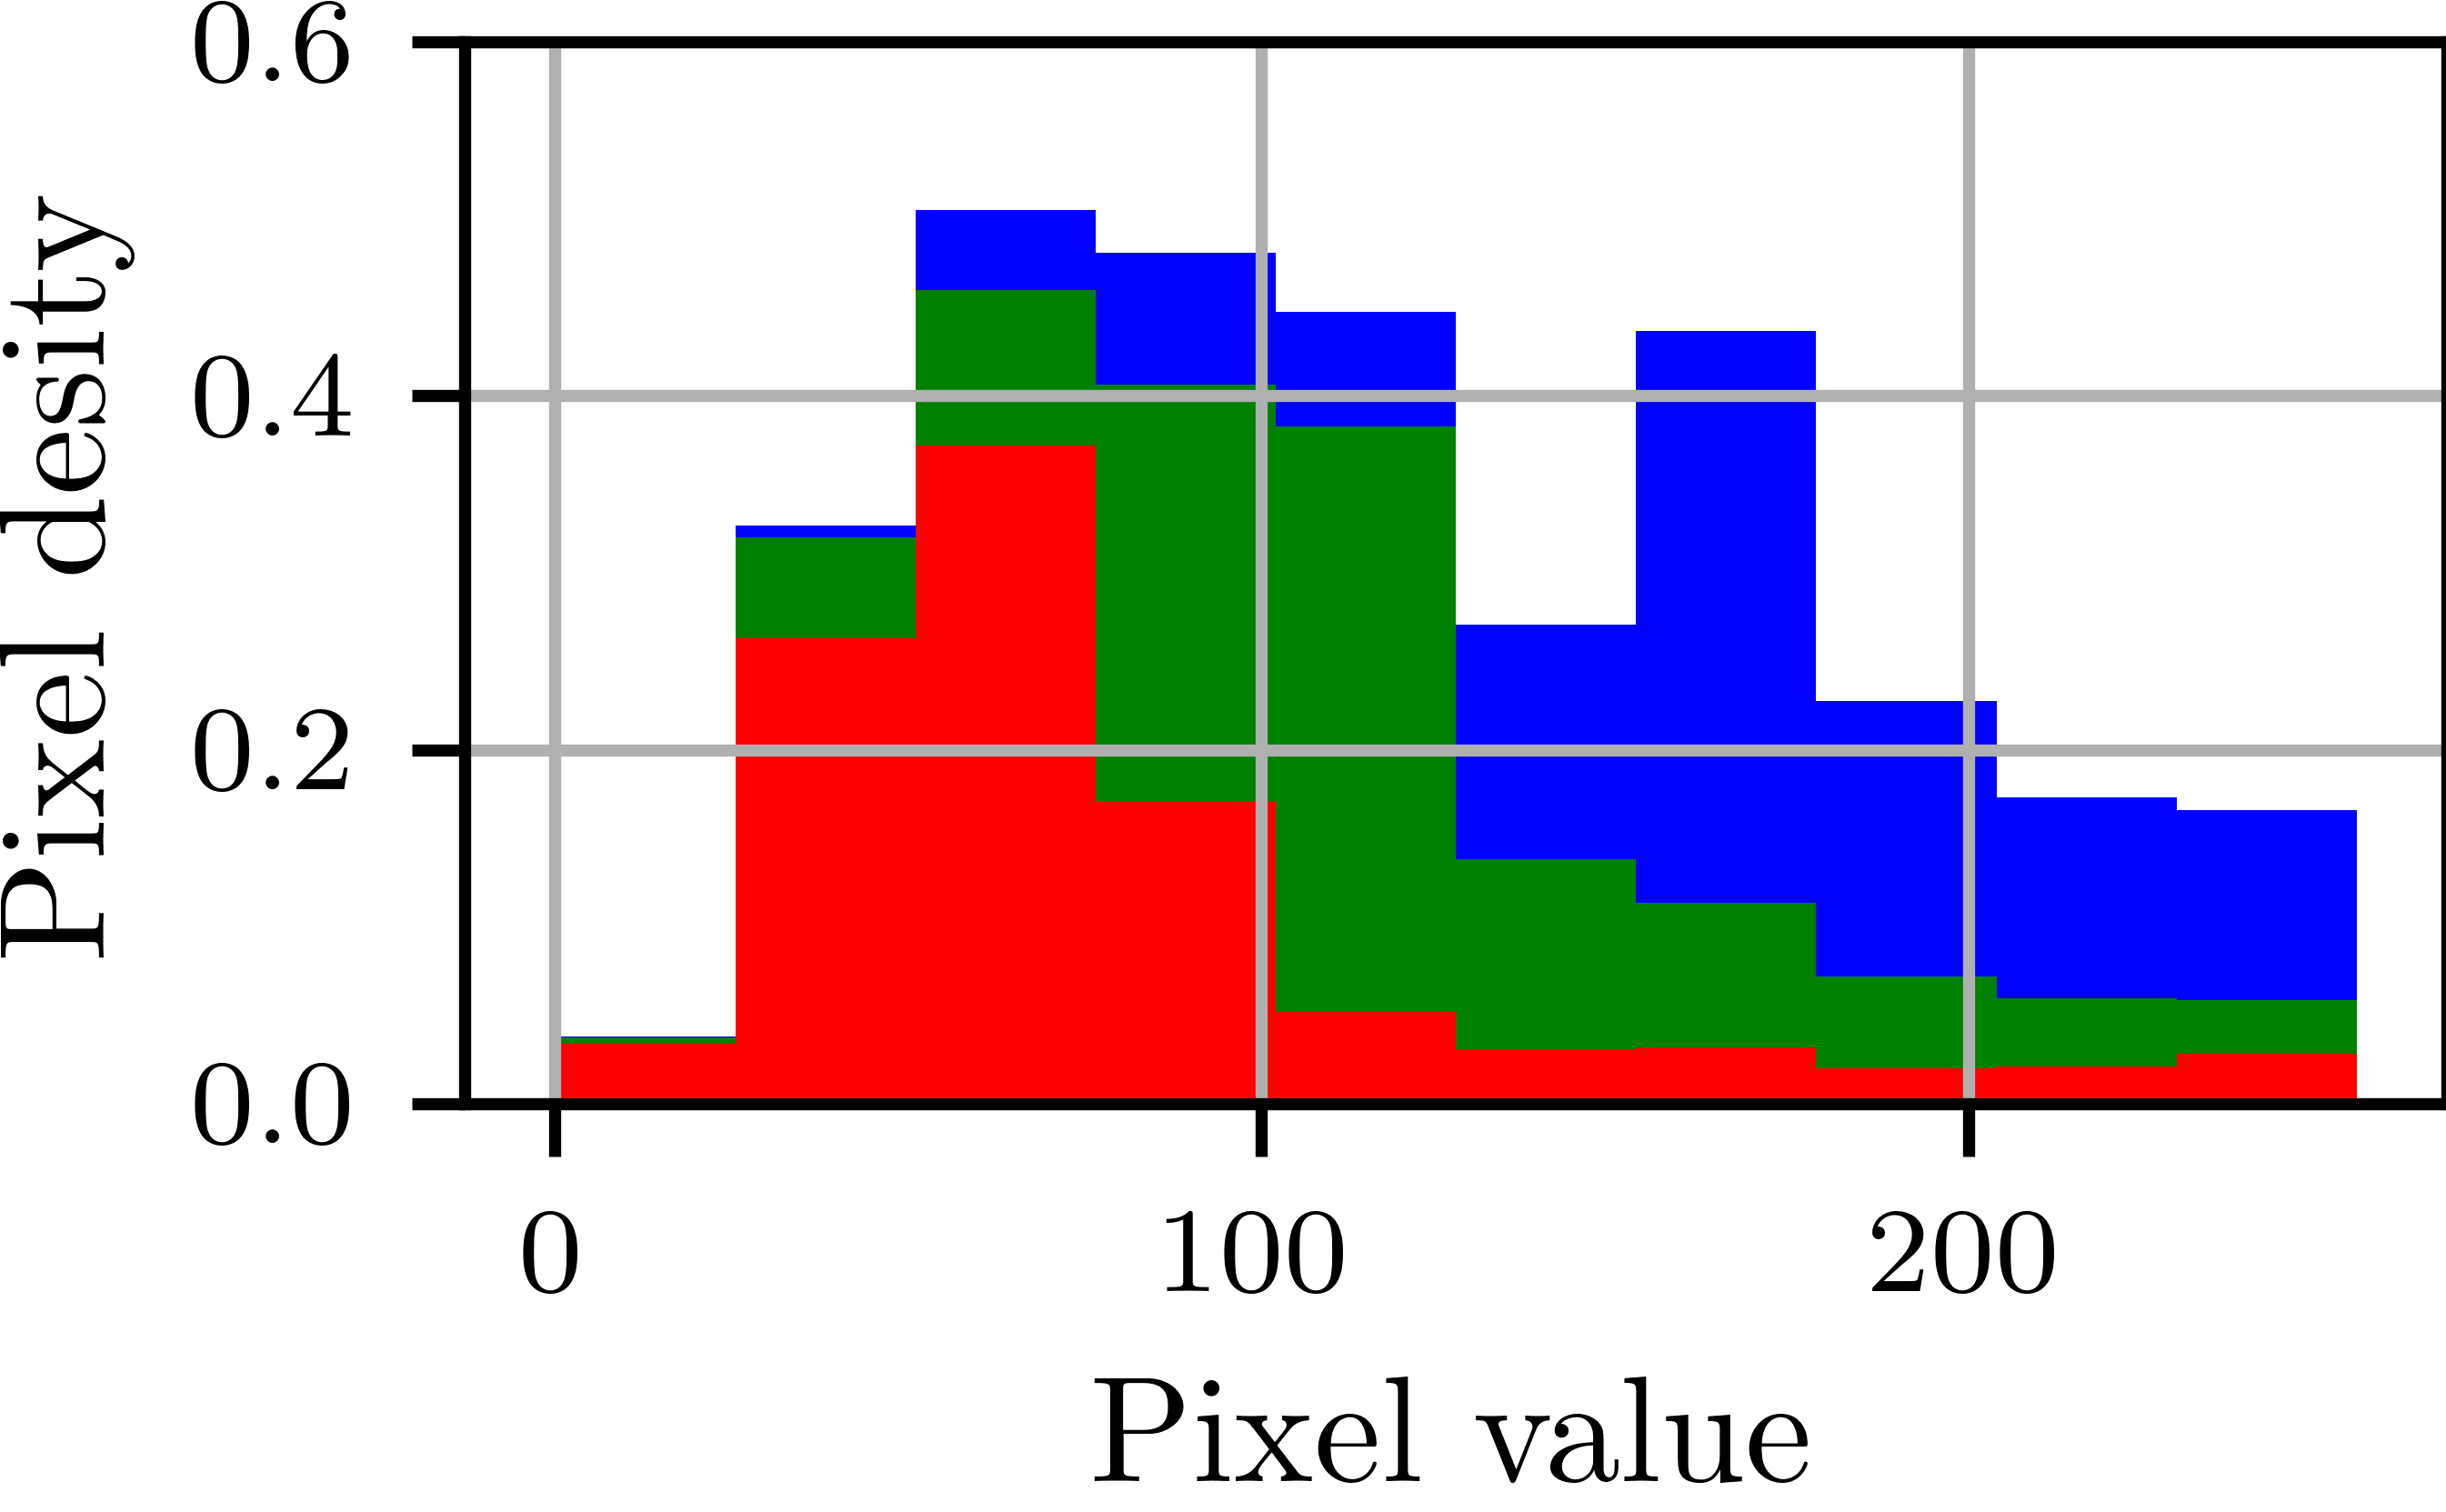
\includegraphics[width=\textwidth]{mountain_single_histogram}
    \end{subfigure}\vspace{10pt}
    
    \begin{subfigure}[t]{\dimexpr0.32\textwidth+20pt\relax}
    	\makebox[20pt]{\raisebox{40pt}{ \small\textbf{\textsf{(c)}} }}%
    	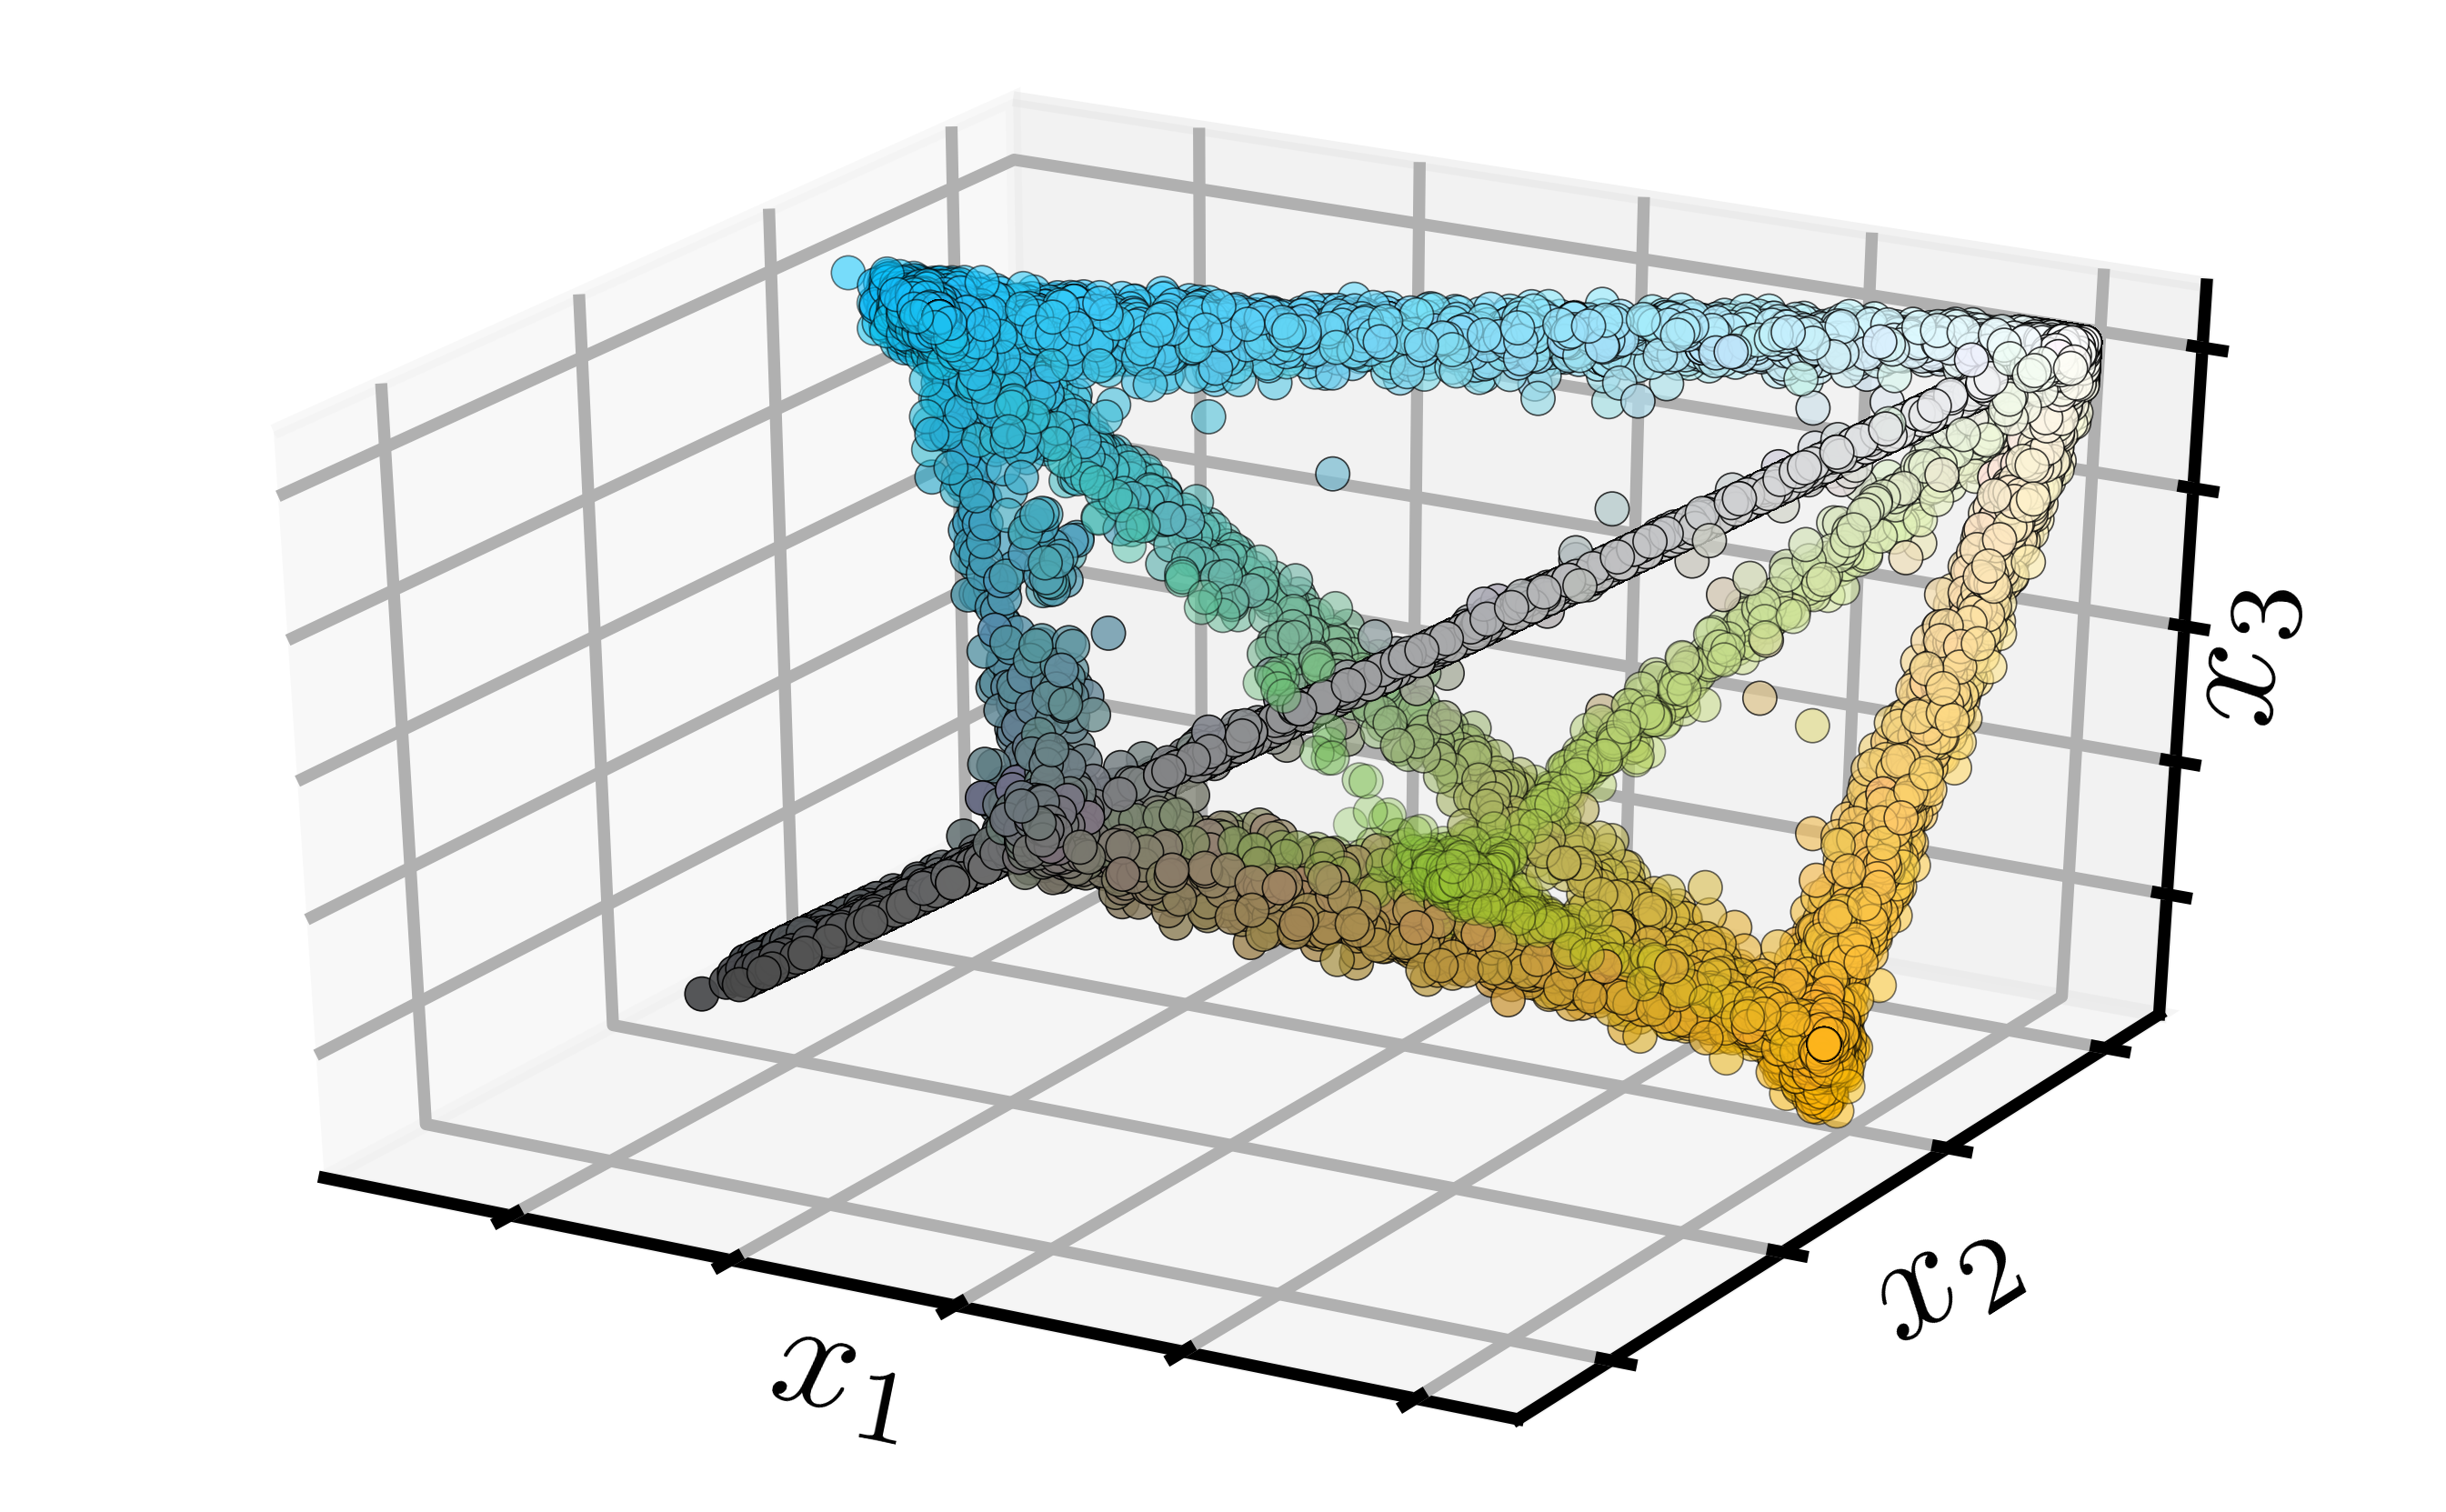
\includegraphics[width=\dimexpr\linewidth-20pt\relax]{tempo_3d_distribution}
    \end{subfigure}~ 
%    \begin{subfigure}[b]{0.32\textwidth}
%        \includegraphics[width=\textwidth]{araras_3d_distribution}
%    \end{subfigure}~
    \begin{subfigure}[b]{0.32\textwidth}
        \includegraphics[width=\textwidth]{clownfish_3d_distribution}
    \end{subfigure}~
    \begin{subfigure}[b]{0.32\textwidth}
        \includegraphics[width=\textwidth]{mountain_3d_distribution}
    \end{subfigure}\vspace{10pt}
    
    \begin{subfigure}[t]{\dimexpr0.32\textwidth+20pt\relax}
    	\makebox[20pt]{\raisebox{40pt}{ \small\textbf{\textsf{(d)}} }}%
    	\includegraphics[width=\dimexpr\linewidth-20pt\relax]{tempo_3d_histogram}
    \end{subfigure}~ 
%    \begin{subfigure}[b]{0.32\textwidth}
%        \includegraphics[width=\textwidth]{araras_3d_histogram}
%    \end{subfigure}~
    \begin{subfigure}[b]{0.32\textwidth}
        \includegraphics[width=\textwidth]{clownfish_3d_histogram}
    \end{subfigure}~
    \begin{subfigure}[b]{0.32\textwidth}
        \includegraphics[width=\textwidth]{mountain_3d_histogram}
    \end{subfigure}\vspace{10pt}
    
    \begin{subfigure}[t]{\dimexpr0.32\textwidth+20pt\relax}
    	\makebox[20pt]{\raisebox{40pt}{ \small\textbf{\textsf{(e)}} }}%
    	\includegraphics[width=\dimexpr\linewidth-20pt\relax]{tempo_3d_signature}
    \end{subfigure}~ 
%    \begin{subfigure}[b]{0.32\textwidth}
%        \includegraphics[width=\textwidth]{araras_3d_signature}
%    \end{subfigure}~
    \begin{subfigure}[b]{0.32\textwidth}
        \includegraphics[width=\textwidth]{clownfish_3d_signature}
    \end{subfigure}~
    \begin{subfigure}[b]{0.32\textwidth}
        \includegraphics[width=\textwidth]{mountain_3d_signature}
    \end{subfigure}\vspace{10pt}
    
    \begin{subfigure}[t]{\dimexpr0.32\textwidth+20pt\relax}
    	\makebox[20pt]{\raisebox{40pt}{ \small\textbf{\textsf{(f)}} }}%
    	\includegraphics[width=\dimexpr\linewidth-20pt\relax]{tempo_color_clusters}
    \end{subfigure}~ 
%    \begin{subfigure}[b]{0.32\textwidth}
%        \includegraphics[width=\textwidth]{araras_color_clusters}
%    \end{subfigure}~
    \begin{subfigure}[b]{0.32\textwidth}
        \includegraphics[width=\textwidth]{clownfish_color_clusters}
    \end{subfigure}~
    \begin{subfigure}[b]{0.32\textwidth}
        \includegraphics[width=\textwidth]{mountain_color_clusters}
    \end{subfigure}\vspace{-5pt}
    
    \begin{subfigure}[t]{\dimexpr0.32\textwidth+20pt\relax}
    	\makebox[20pt]{\raisebox{25pt}{}}%
    	\includegraphics[width=\dimexpr\linewidth-20pt\relax]{tempo_bar_signature}
    \end{subfigure}~ 
%    \begin{subfigure}[b]{0.32\textwidth}
%        \includegraphics[width=\textwidth]{araras_bar_signature}
%    \end{subfigure}~
    \begin{subfigure}[b]{0.32\textwidth}
        \includegraphics[width=\textwidth]{clownfish_bar_signature}
    \end{subfigure}~
    \begin{subfigure}[b]{0.32\textwidth}
        \includegraphics[width=\textwidth]{mountain_bar_signature}
    \end{subfigure}
                    
	\caption{Different representations of color information. {\small \textsf{\textbf{(a)}}} input color image , {\small \textsf{\textbf{(b)}}} single-channel color histogram , {\small \textsf{\textbf{(c)}}} 3-d color distribution , {\small \textsf{\textbf{(d)}}} 3-d color histogram , {\small \textsf{\textbf{(e)}}} 3-d color signature , {\small \textsf{\textbf{(f)}}} color signature clusters .}\label{fig:color_image_representations}    
\end{figure}




\section{Texture}

\section{Texture characterization}

\begin{figure}[!ht]
    \centering
    \begin{subfigure}[b]{0.19\textwidth}
        \includegraphics[width=\textwidth]{brodatz_skin}
        \caption{}
    \end{subfigure}
    %~ %add desired spacing between images, e. g. ~, \quad, \qquad, \hfill etc. 
      %(or a blank line to force the subfigure onto a new line)
    \begin{subfigure}[b]{0.19\textwidth}
        \includegraphics[width=\textwidth]{brodatz_three}
        \caption{}
    \end{subfigure} 
    %~ %add desired spacing between images, e. g. ~, \quad, \qquad, \hfill etc. 
      %(or a blank line to force the subfigure onto a new line)    
    \begin{subfigure}[b]{0.19\textwidth}
        \includegraphics[width=\textwidth]{brodatz_wall}
        \caption{}
    \end{subfigure}
    %~ %add desired spacing between images, e. g. ~, \quad, \qquad, \hfill etc. 
      %(or a blank line to force the subfigure onto a new line)
    \begin{subfigure}[b]{0.19\textwidth}
        \includegraphics[width=\textwidth]{brodatz_vlines}
        \caption{}
    \end{subfigure}
    %~ %add desired spacing between images, e. g. ~, \quad, \qquad, \hfill etc. 
      %(or a blank line to force the subfigure onto a new line)
    \begin{subfigure}[b]{0.19\textwidth}
        \includegraphics[width=\textwidth]{brodatz_sponge}
        \caption{}
    \end{subfigure}\\
    
    \begin{subfigure}[b]{0.19\textwidth}
        \includegraphics[width=\textwidth]{brodatz_tissue}
        \caption{}
    \end{subfigure}
    %~ %add desired spacing between images, e. g. ~, \quad, \qquad, \hfill etc. 
      %(or a blank line to force the subfigure onto a new line)
    \begin{subfigure}[b]{0.19\textwidth}
        \includegraphics[width=\textwidth]{brodatz_cafe}
        \caption{}
    \end{subfigure} 
    %~ %add desired spacing between images, e. g. ~, \quad, \qquad, \hfill etc. 
      %(or a blank line to force the subfigure onto a new line)    
    \begin{subfigure}[b]{0.19\textwidth}
        \includegraphics[width=\textwidth]{brodatz_crystal}
        \caption{}
    \end{subfigure}
    %~ %add desired spacing between images, e. g. ~, \quad, \qquad, \hfill etc. 
      %(or a blank line to force the subfigure onto a new line)
    \begin{subfigure}[b]{0.19\textwidth}
        \includegraphics[width=\textwidth]{brodatz_flowers}
        \caption{}
    \end{subfigure}
    %~ %add desired spacing between images, e. g. ~, \quad, \qquad, \hfill etc. 
      %(or a blank line to force the subfigure onto a new line)
    \begin{subfigure}[b]{0.19\textwidth}
        \includegraphics[width=\textwidth]{brodatz_paint}
        \caption{}
    \end{subfigure}    
                  
    \caption{ Examples of texture images and its classification. [{\small \textsf{\textbf{(a) (b) (e) (h)}}}] nautural textures, [{\small \textsf{\textbf{(c) (d) (f) (g) (i) (j)}}}] man-made textures, [{\small \textsf{\textbf{(c) (d)}}}] regular textures, [{\small \textsf{\textbf{(g) (h)}}}] stochastic textures, [{\small \textsf{\textbf{(c) (d)}}}] homogeneous, [{\small \textsf{\textbf{(a) (b) (f) (g) (h)}}}] weakly-homogeneous, [{\small \textsf{\textbf{(i) (j)}}}] inhomogeneous.}\label{fig:texture_images}    
\end{figure}


\begin{itemize}
	\item Natural and artificial 
	\item Regular, stochastic
	\item Homogeneous, non-homogeneous, in-homogeneous
\end{itemize}



There is a disagreement in the definition of texture in the field of computer vision. It is possible to give a mathematical definition based on its statistical properties, however, these properties are very imprecise and/or restrictive to adapt to the diversity of existing textures.

The definition that we support is based on an experimental finding: a texture is a field of the image that appears as a coherent and homogeneous domain, that is, it forms a whole for an observer. In fact, it is this property of coherence of the texture placed in the context of being perceived as a homogeneous whole for the human eye that is most often sought for image processing, either with the aim of isolating textures, to segment the image or for the recognition of regions.

Some examples of natural textures are shown in the figure. These images come from the reference work Brodatz and show the possible variety of textures that are commonly used to test different algorithms and methods of vision.

The perception of textures is a key property of human vision. Although there is still no generalized definition, we can define texture as a measure of coarseness, contrast, directionality, line similarity, regularity and roughness. Therefore, the features that chracterize texture attempt to capture the granularity and repetition of perceptually similar patterns of surfaces within a region of the image, such that a human observer perceives the region as homogeneous.
Unlike color, texture information is not a purely pixel-level property. Texture implies the notion of spatial extent, that is, that the spatial variation of intensities of a group of pixels generate textures in the images.

There are numerous studies that review, compare and organize the work of texture analysis in different ways \citep{Materka.Strzelecki:Report:1998}, \citep{Zhang.Tan:PR:2002}, \citep{Bharati.Liu.ea:CILS:2004},\citep{Lukashevich.Sadykhov:ICPCI:2012}, \citep{Humeau-Heurtier:IEEEAccess:2019}. One possible organization is based on its operating principle, which classifies the texture characterization techniques into: statistical methods, structural method, model-based methods, transform-based methods, graph-based methods, learning-based methods and entropy-based methods. In this chapter we review five of the most widely used methods in the literature and their techniques for extracting textures fearures.

% \begin{enumerate}[noitemsep]%,topsep=0pt
%	\item Statistical methods
%	\item Structural methods
%	\item Model-based methods
%	\item Transform-based methods
%	\item Graph-based methods
%	\item Learning-based methods
%	\item Entropy-based methods
%\end{enumerate}
%	

\subsection{Statistical Methods}
Statistical methods contemplate that textures are determined by the way the gray levels are distributed over the pixels of an image. In these methods, the gray level distribution of the image is represented by a histogram.

A first approach in this category is the histogram properties analysis \citep{Aggarwal.K.Agrawal:JSIP:2012}. The first-order statistics properties are the mean and the Central Moments of the 1D histogram, that is, the variance, skewness, and kurtosis. These properties provide information on the distribution of the gray levels of the image from a global point of view, taking into account individually the gray level of the pixels. Hoewever, they do not provide any information on how the gray level of a pixel at a given location statistically affects the gray level value of another pixel at a relative location from the reference pixel.
The second-order statistical properties explore this option ang give a description of the texture, based on the comparison of intensity values of two pixels. In this case the Co-Occurrence matrix \citep{Haralick.Shanmugam.ea:TSMC:1973} is the second-level histogram that maps the intensity distribution of the pixels. Some of the texture features extracted from the second-order statistics are Angular Second Moment (ASM), Contrast, Correlation, Homogeneity, Entropy and Energy.

Local Binary Patterns (LBP) \citep{Ojala.Pietikainen.ea:PR:1996} are another technique for obtaining second-level histograms. This approach summarizes the spatial structure and local contrast of an image within a binary pattern, comparing the gray level of each pixel with its neighborhood. If the intensity value of the central pixel is greater than its neighbor, then it is denoted by 1, otherwise by 0. Subsequently, a binary array is constructed, following a consistent ordering of the neighboring values, which is transformed to decimal number and stored in a new array. The process of thresholding, construction of binary strings, binary to decimal transformation, and storing of decimal output is performed for all pixels in the image, resulting in an LPB image. Finally the second-level histogram for texture chraracterization is obtained from this resulting LBP image.

\subsection{Structural Methods}
The structural methods are based on the decomposition of the image in basic units, i.e., in elements, low-level primitives o texels. Such units can be points, lines, regions, or shapes. The basic units and their spatial arrangement in the image are used to characterize the textures. These approaches consider that textures are patterns formed by replication, more or less regular, of a basic unit. The arrangement of the primitives allows obtaining geometric relationships and subsequently statistical properties that serve serve to characterize textures. Structural tecniques aim to determine the textual primitive and define the location rules.

Dpends on the application, structural tecniques differ according to the choice of primitives. Some of the commonly considered primitives are pixels, regions of uniform intensity, line segments, or peaks in the gray level distribution. For the recovery of these primitives, highly known approaches are generally used, for example, the SIFT (Scale Invariant Feature Trasform) operator in the case of characteristic points and the contour detectors, such as Sobel and Canny, for line and edge recovery. On the other hand, the primitive's measurements and statistics most commonly used are intensity, orientation, elongation, curvature, compactness, among others.

\subsection{Model-based Methods}
This group of methods stipulates that the textures can be described by some mathematical model. This category is mainly subdivided into two approaches: stochastics and fractals.

Stochastic methods for texture modeling are very popular, in particular random field models. In this context, a texture model is a parametric family of spatially homogeneous random fields, which depend on a series of hyperparameters \citep{Winkler:Book:2003}. Inside such a family a specific texture can be characterized by a special set of hyperparameters that captures its characteristic features. According to the properties of the random fields, some of the models used for the characterization of texture are Markov Random Field (MRF) \citep{Hassner.Sklansky:CGIM:1980, Cross.Jain:PAMI:1983}, Gibbs Random Field (GRF) \citep{Derin.Cole:CVGIM:1986}, Conditional Random Field (CRF), Gaussian Markov Random Field (GMRF) \citep{Cohen.Fan.ea:PAMI:1991}.

Within the category of stochastic approaches, there is a group of techniques that use probabilistic approaches and mathematical morphology operators for the modeling of random textures \citep{Serra:CGIM:1980}, \citep{Cord.Bach.ea:JoM:2010}.

Fractal models consider textures as complex chaotic systems, so they exhibit fractal behavior. Textures, as fractal objects, have identical shape and statistical characteristics at different scales. Fractal geometry relies on self similarity across multiple scales and is measured with the fractal dimension. Fractal model-based approaches aim to determine fractal dimension, find fractal geometry, and calculate fractal measurements for the description of textures in images.


\subsection{Transform-based Methods}
Transform methods map an image to a space within which the textures are characterizable. The peculiarity is that the new space coordinates allow the interpretation of the textures because they reflect the texture properties, for example, the log-polar coordinates in the case of Gabor transform, they reflect the periodicity and orientation of the textures present in an image.

Within this category, one of the most notable methods for the extraction of texture features are Law's filter banks \citep{Laws:IUW:1979, Laws:IPMG:1980, Laws:Report:1980}. There are also the approaches based on the Fourier transform \citep{Ursani.Kpalma.ea:ICMV:2007}, where it is used to decompose the image into its frequency components. Following the same principle, there are the approaches based on Gabor decomposition \citep{Gabor:JIEE:1946} and those based on wavelets \citep{Arivazhagan.Ganesan:PR:2003}, which analyze the content of a texture not only in the frequency domain, but also in the spatial domain. On the one hand, the Gabor filter is defined as a sinusoidal wave plane modulated Gaussian kernel, which can be adapted in frequency, orientation and bandwidth. For its part, the wavelet transform allows the analysis of the texture in the frequency and spatial domain by means of the dilation and translation, respectively, of a mother wavelet.

\subsection{Learning-based Methods}
The methods for the extraction of texture features based on learning are relatively new with respect to the other methods mentioned in this work.
This category of approaches can be divided into two subclasses: the visual dictionary methods and the deep learning methods.

Visual dictionary methods are motivated by natural language processing algorithms. In this case, the aim is to generate a codebook or dictionary that contains basic geometric elements of the images, also called \textit{textons}. In the document processing analogy, textons correspond to words; so an image can be described by the repetition (organized or not) of a set of textons.

There are different strategies for calculating textons \citep{Zhu.Guo.ea:IJCV:2005}. For example, the approaches based on generative models, where an image is considered to be a linear combination of some base images. Such base images are represented by Gabor or Laplacian-of-Gaussian (LoG) functions and other wavelet transforms. Following the principle of generative models, textons are the base functions learned from a large number of image patches.
Other approaches to obtaining textons are based on discriminative modeling. In this case, the base functions are rotated and scaled filters that form a family which is convolved with the image. The responses of the filters form a feature space  in which it is possible to form clusters. Each cluster center then corresponds to a texton. To obtain a texton dictionary, it is necessary to obtain the feature space and the cluster centers from a group of training images.

Models based on deep learning use Convolutional Neural Networks (CNNs) for the extraction and representation of image features. CNNs consist of multiple locally connected layers which covolve kernels over the entire image. These approaches analyze the information of a group of images to generate a model. The characteristics of the learned model are a function of the input images, which in the case of the study of texture, is expected to generalize the properties of granularity, frequency, orientation, etc. of patterns in the training dataset.


%\section{Conclusions}

